%%%%%%%%%%%%%%%%%%%%%%%%%%%%%%%%%%%%%%%%%%%%%%%
%
% Template per Elaborato di Laurea
% DISI - Dipartimento di Ingegneria e Scienza dell’Informazione
%
% update 2015-09-10
%
% Per la generazione corretta del 
% pdflatex nome_file.tex
% bibtex nome_file.aux
% pdflatex nome_file.tex
% pdflatex nome_file.tex
%
%%%%%%%%%%%%%%%%%%%%%%%%%%%%%%%%%%%%%%%%%%%%%%%



% formato FRONTE RETRO
\documentclass[epsfig,a4paper,11pt,titlepage,twoside,openany]{book}
\usepackage{epsfig}
\usepackage{plain}
\usepackage{setspace}
\usepackage[paperheight=29.7cm,paperwidth=21cm,outer=1.5cm,inner=2.5cm,top=2cm,bottom=2cm]{geometry} % per definizione layout
\usepackage{titlesec} % per formato custom dei titoli dei capitoli
\usepackage[hidelinks]{hyperref}
\hypersetup{
    % colorlinks=false,
    % linkcolor=blue,
    % filecolor=magenta,      
    % urlcolor=cyan,
    pdftitle={Berardo-Cristiano-2024-2025},
    pdfpagemode=FullScreen,
    }
\usepackage{svg}
\usepackage{amsmath}
\usepackage{booktabs}
%%%%%%%%%%%%%%
% supporto lettere accentate
%
%\usepackage[latin1]{inputenc} % per Windows;
\usepackage[utf8x]{inputenc} % per Linux (richiede il pacchetto unicode);
%\usepackage[applemac]{inputenc} % per Mac.

\singlespacing

\usepackage[italian]{babel}

\begin{document}

  % nessuna numerazione
  \pagenumbering{gobble} 
  \pagestyle{plain}

\thispagestyle{empty}

\begin{center}
  \begin{figure}[h!]
    \centerline{
\psfig{file=./img/marchio_unitrento_colore_it_202002.eps,width=0.6\textwidth}}
  \end{figure}

  \vspace{2 cm} 

  \LARGE{Dipartimento di Ingegneria e Scienza dell'Informazione\\}

  \vspace{1 cm} 
  \Large{Corso di Laurea in\\
    %Informatica
    %Ingegneria dell'Informazione e delle Comunicazioni
    %Ingegneria dell'Informazione e Organizzazione d'Impresa
    %Ingegneria Elettronica e delle Telecomunicazioni
    Ingegneria Informatica, delle Comunicazioni ed Elettronica
  }

  \vspace{2 cm} 
  \Large\textsc{Elaborato finale\\} 
  \vspace{1 cm} 
  \Huge\textsc{Modellazione di minacce informatiche in ambiente Smart Grid Cloudificato\\}
  % \Large{\it{in ambiente Smart Grid Cloudificato}}


  \vspace{2 cm} 
  \begin{tabular*}{\textwidth}{ c @{\extracolsep{\fill}} c }
  \Large{Supervisore} & \Large{Laureando}\\
  \Large{Prof. Domenico Siracusa}& \Large{Berardo Cristiano - 234428}\\
  % & \Large{Mat. 234428}
  \end{tabular*}

  \vspace{2 cm} 

  \Large{Anno accademico 2024/2025}
  
\end{center}



  \clearpage
 
%%%%%%%%%%%%%%%%%%%%%%%%%%%%%%%%%%%%%%%%%%%%%%%%%%%%%%%%%%%%%%%%%%%%%%%%%%
%%%%%%%%%%%%%%%%%%%%%%%%%%%%%%%%%%%%%%%%%%%%%%%%%%%%%%%%%%%%%%%%%%%%%%%%%%
%% Nota
%%%%%%%%%%%%%%%%%%%%%%%%%%%%%%%%%%%%%%%%%%%%%%%%%%%%%%%%%%%%%%%%%%%%%%%%%%
%% Sezione Ringraziamenti opzionale
%%%%%%%%%%%%%%%%%%%%%%%%%%%%%%%%%%%%%%%%%%%%%%%%%%%%%%%%%%%%%%%%%%%%%%%%%%
%%%%%%%%%%%%%%%%%%%%%%%%%%%%%%%%%%%%%%%%%%%%%%%%%%%%%%%%%%%%%%%%%%%%%%%%%%
  \thispagestyle{empty}

\begin{center}
  {\bf \Huge Ringraziamenti}
\end{center}

\vspace{4cm}


\emph{
  ...thanks to...
}

  \clearpage
  \pagestyle{plain} % nessuna intestazione e pie pagina con numero al centro

  
  % inizio numerazione pagine in numeri arabi
  \mainmatter

%%%%%%%%%%%%%%%%%%%%%%%%%%%%%%%%%%%%%%%%%%%%%%%%%%%%%%%%%%%%%%%%%%%%%%%%%%
%%%%%%%%%%%%%%%%%%%%%%%%%%%%%%%%%%%%%%%%%%%%%%%%%%%%%%%%%%%%%%%%%%%%%%%%%%
%% Nota
%%%%%%%%%%%%%%%%%%%%%%%%%%%%%%%%%%%%%%%%%%%%%%%%%%%%%%%%%%%%%%%%%%%%%%%%%%
%% Si ricorda che il numero massimo di facciate e' 30.
%% Nel conteggio delle facciate sono incluse 
%%   indice
%%   sommario
%%   capitoli
%% Dal conteggio delle facciate sono escluse
%%   frontespizio
%%   ringraziamenti
%%   allegati    
%%%%%%%%%%%%%%%%%%%%%%%%%%%%%%%%%%%%%%%%%%%%%%%%%%%%%%%%%%%%%%%%%%%%%%%%%%
%%%%%%%%%%%%%%%%%%%%%%%%%%%%%%%%%%%%%%%%%%%%%%%%%%%%%%%%%%%%%%%%%%%%%%%%%%

    % indice
    \tableofcontents
    \clearpage
    
    
          
    % gruppo per definizone di successione capitoli senza interruzione di pagina
    \begingroup
      % nessuna interruzione di pagina tra capitoli
      % ridefinizione dei comandi di clear page
      \renewcommand{\cleardoublepage}{} 
      \renewcommand{\clearpage}{} 
      % redefinizione del formato del titolo del capitolo
      % da formato
      %   Capitolo X
      %   Titolo capitolo
      % a formato
      %   X   Titolo capitolo
      
      \titleformat{\chapter}
        {\normalfont\Huge\bfseries}{\thechapter}{1em}{}
        
      \titlespacing*{\chapter}{0pt}{0.59in}{0.02in}
      \titlespacing*{\section}{0pt}{0.20in}{0.02in}
      \titlespacing*{\subsection}{0pt}{0.10in}{0.02in}
      
      % sommario
      \chapter*{Sommario} % senza numerazione
\label{sommario}

\addcontentsline{toc}{chapter}{Sommario} % da aggiungere comunque all'indice

% Lorem ipsum dolor sit amet, consectetur adipiscing elit. Donec sed nunc orci. Aliquam nec nisl vitae sapien pulvinar dictum quis non urna. Suspendisse at dui a erat aliquam vestibulum. Quisque ultrices pellentesque pellentesque. Pellentesque egestas quam sed blandit tempus. Sed congue nec risus posuere euismod. Maecenas ut lacus id mauris sagittis egestas a eu dui. Class aptent taciti sociosqu ad litora torquent per conubia nostra, per inceptos himenaeos. Pellentesque at ultrices tellus. Ut eu purus eget sem iaculis ultricies sed non lorem. Curabitur gravida dui eget ex vestibulum venenatis. Phasellus gravida tellus velit, non eleifend justo lobortis eget.


%   Sommario è un breve riassunto del lavoro svolto dove si descrive l'obiettivo, l'oggetto della tesi, le 
% metodologie e le tecniche usate, i dati elaborati e la spiegazione delle conclusioni alle quali siete arrivati.  

% Il sommario dell’elaborato consiste al massimo di 3 pagine e deve contenere le seguenti informazioni:
% \begin{itemize}
%   \item contesto e motivazioni 
%   \item breve riassunto del problema affrontato
%   \item tecniche utilizzate e/o sviluppate
%   \item risultati raggiunti, sottolineando il contributo personale del laureando/a
% \end{itemize}



La transizione globale verso un paradigma energetico sostenibile ha accelerato l'evoluzione delle reti elettriche tradizionali in Smart Grid. Questa trasformazione, caratterizzata dall'integrazione di fonti rinnovabili e dalla partecipazione attiva dei consumatori (\textit{prosumer}), impone requisiti di scalabilità, resilienza e capacità di elaborazione dati che le architetture IT convenzionali faticano a soddisfare. In risposta, le infrastrutture critiche stanno adottando sempre più il paradigma \textit{Cloud-Native}, che promette agilità, efficienza e robustezza attraverso tecnologie come la containerizzazione e l'orchestrazione con Kubernetes.


Tuttavia, se da un lato l'adozione del \textit{cloud} offre vantaggi significativi, dall'altro introduce nuove e complesse superfici di attacco, esponendo le operazioni della rete energetica a minacce informatiche sofisticate. La sicurezza di tali sistemi diventa, quindi, una priorità non negoziabile.



Il presente elaborato si pone l'obiettivo di analizzare e modellare sistematicamente le minacce informatiche in un'architettura Smart Grid progettata secondo i principi \textit{Cloud-Native}. Il lavoro si articola in tre fasi principali:


\begin{enumerate}
    \item \textbf{Analisi del Dominio:} Viene presentata un'analisi dettagliata dell'architettura della Smart Grid, dai componenti di produzione fino al dominio del consumatore e operazionale, evidenziando le tecnologie chiave come AMI, SCADA, EMS e DMS.
    \item \textbf{Proposta Architetturale:} Viene definito un modello architetturale \textit{Cloud-Native} per la Smart Grid, basato su una federazione di cluster Kubernetes isolati (\textit{Trusted Boundaries}) che gestiscono i diversi domini funzionali (AMI, DMS, EMS), garantendo robustezza e autonomia operativa.
    \item \textbf{Modellazione delle Minacce:} Viene applicata la metodologia formale del \textit{Threat Modeling}. Utilizzando un Diagramma di Flusso dei Dati (DFD) per rappresentare l'architettura, si applica il framework STRIDE (\textit{\textbf{S}poofing, \textbf{T}ampering, \textbf{R}epudiation, \textbf{I}nformation Disclosure, \textbf{D}enial of Service, \textbf{E}levation of Privilege}) per identificare, classificare e analizzare sistematicamente le potenziali minacce.
\end{enumerate}



L'analisi ha permesso di individuare vulnerabilità critiche, come attacchi di \textit{Tampering} ai dati provenienti dai PMU, \textit{Denial of Service} contro i sistemi SCADA ospitati nel \textit{cloud} e attacchi di \textit{Elevation of Privileg} e per il controllo coordinato di dispositivi remoti. Per ciascuna minaccia significativa, vengono proposte strategie di mitigazione e contromisure di sicurezza specifiche per il contesto \textit{Cloud-Native}, tra cui l'uso di database WORM, la segmentazione dei privilegi tramite RBAC e l'adozione di \textit{best practice} per la sicurezza dei container e dei cluster.


Il contributo principale di questa tesi risiede nell'applicazione strutturata di una metodologia di sicurezza proattiva ("\textit{Secure by Desig}n") a un'infrastruttura critica moderna, fornendo un modello concreto per l'analisi dei rischi in sistemi ciber-fisici complessi e distribuiti.

%%%%%%%%%%%%%%%%%%%%%%%%%%%%%%%%%%%%%%%%%%%%%%%%%%%%%%%%%%%%%%%%%%%%%%%%%%
%%%%%%%%%%%%%%%%%%%%%%%%%%%%%%%%%%%%%%%%%%%%%%%%%%%%%%%%%%%%%%%%%%%%%%%%%%
%% Nota
%%%%%%%%%%%%%%%%%%%%%%%%%%%%%%%%%%%%%%%%%%%%%%%%%%%%%%%%%%%%%%%%%%%%%%%%%%
%% Sommario e' un breve riassunto del lavoro svolto dove si descrive 
%% l’obiettivo, l’oggetto della tesi, le metodologie e 
%% le tecniche usate, i dati elaborati e la spiegazione delle conclusioni 
%% alle quali siete arrivati.
%% Il sommario dell’elaborato consiste al massimo di 3 pagine e deve contenere le seguenti informazioni: 
%%   contesto e motivazioni
%%   breve riassunto del problema affrontato
%%   tecniche utilizzate e/o sviluppate
%%   risultati raggiunti, sottolineando il contributo personale del laureando/a
%%%%%%%%%%%%%%%%%%%%%%%%%%%%%%%%%%%%%%%%%%%%%%%%%%%%%%%%%%%%%%%%%%%%%%%%%%
%%%%%%%%%%%%%%%%%%%%%%%%%%%%%%%%%%%%%%%%%%%%%%%%%%%%%%%%%%%%%%%%%%%%%%%%%%      
      
      %%%%%%%%%%%%%%%%%%%%%%%%%%%%%%%%
      % lista dei capitoli
      %
      % \input oppure \include
      %
      \newpage
\chapter{Smart Grid: architettura, componenti ed evoluzione}

\section{Introduzione alle Smart Grid}



Una Smart Grid - Rete Intelligente - è l'evoluzione della tradizionale rete elettrica. Si basa su componenti avanzati di \textbf{rilevamento}, \textbf{comunicazione} e \textbf{decisione} per ottenere una trasmissione e distribuzione di energia \textbf{sicura}, \textbf{efficiente} e \textbf{resiliente}. \cite{en15186799}


L'aumento di anno in anno di fonti rinnovabili ha portato ad una crescita significativa della generazione di energia distribuita, ovvero la produzione di energia tramite piccoli impianti connessi alla rete di distribuzione elettrica. In questo contesto di flussi non più monodirezionali, bensì bidirezionali, l'utilizzo di Smart Grid possono essere di grande aiuto per le aziende di Trasmissione e Distribuzione dell'energia elettrica. \cite{Enel}


\begin{figure}[h!]
    \centering
    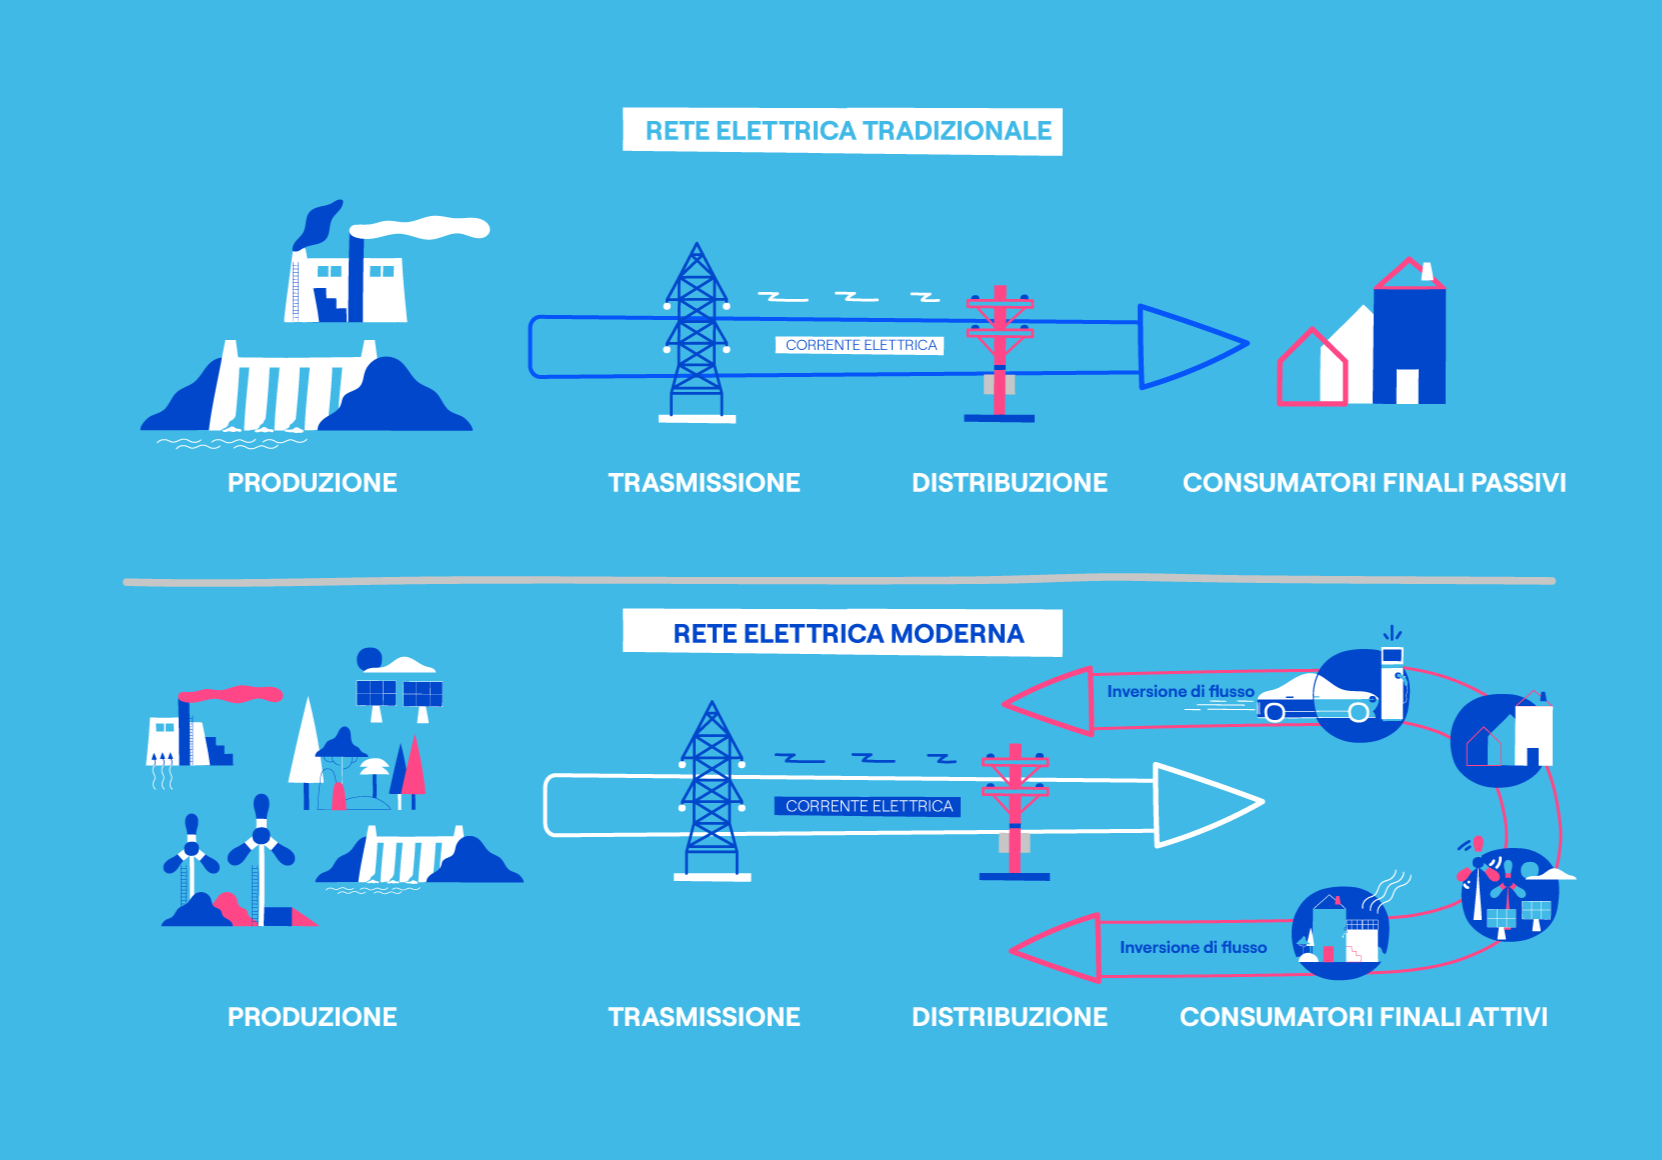
\includegraphics[width=0.8\linewidth]{img/Smart-Grid-EDistribuzione2.png}
    \caption{Confronto rete tradizionale e rete intelligente}
    \label{fig:TraditionalGridVSSmartrGrid}
\end{figure}


Come si può vedere nella Figura \ref{fig:TraditionalGridVSSmartrGrid} la Smart Grid si compone di 4 parti fondamentali: la \textit{Produzione}, la 
\textit{Trasmissione}, la \textit{Distribuzione} e infine le \textit{Utenze}.

% \begin{center}
%     \textit{Produzione} - \textit{Trasmissione} - \textit{Distribuzione} - \textit{Utenze}
% \end{center}

\newpage
\subsection{Produzione}

\begin{figure}[t]
    \centering
    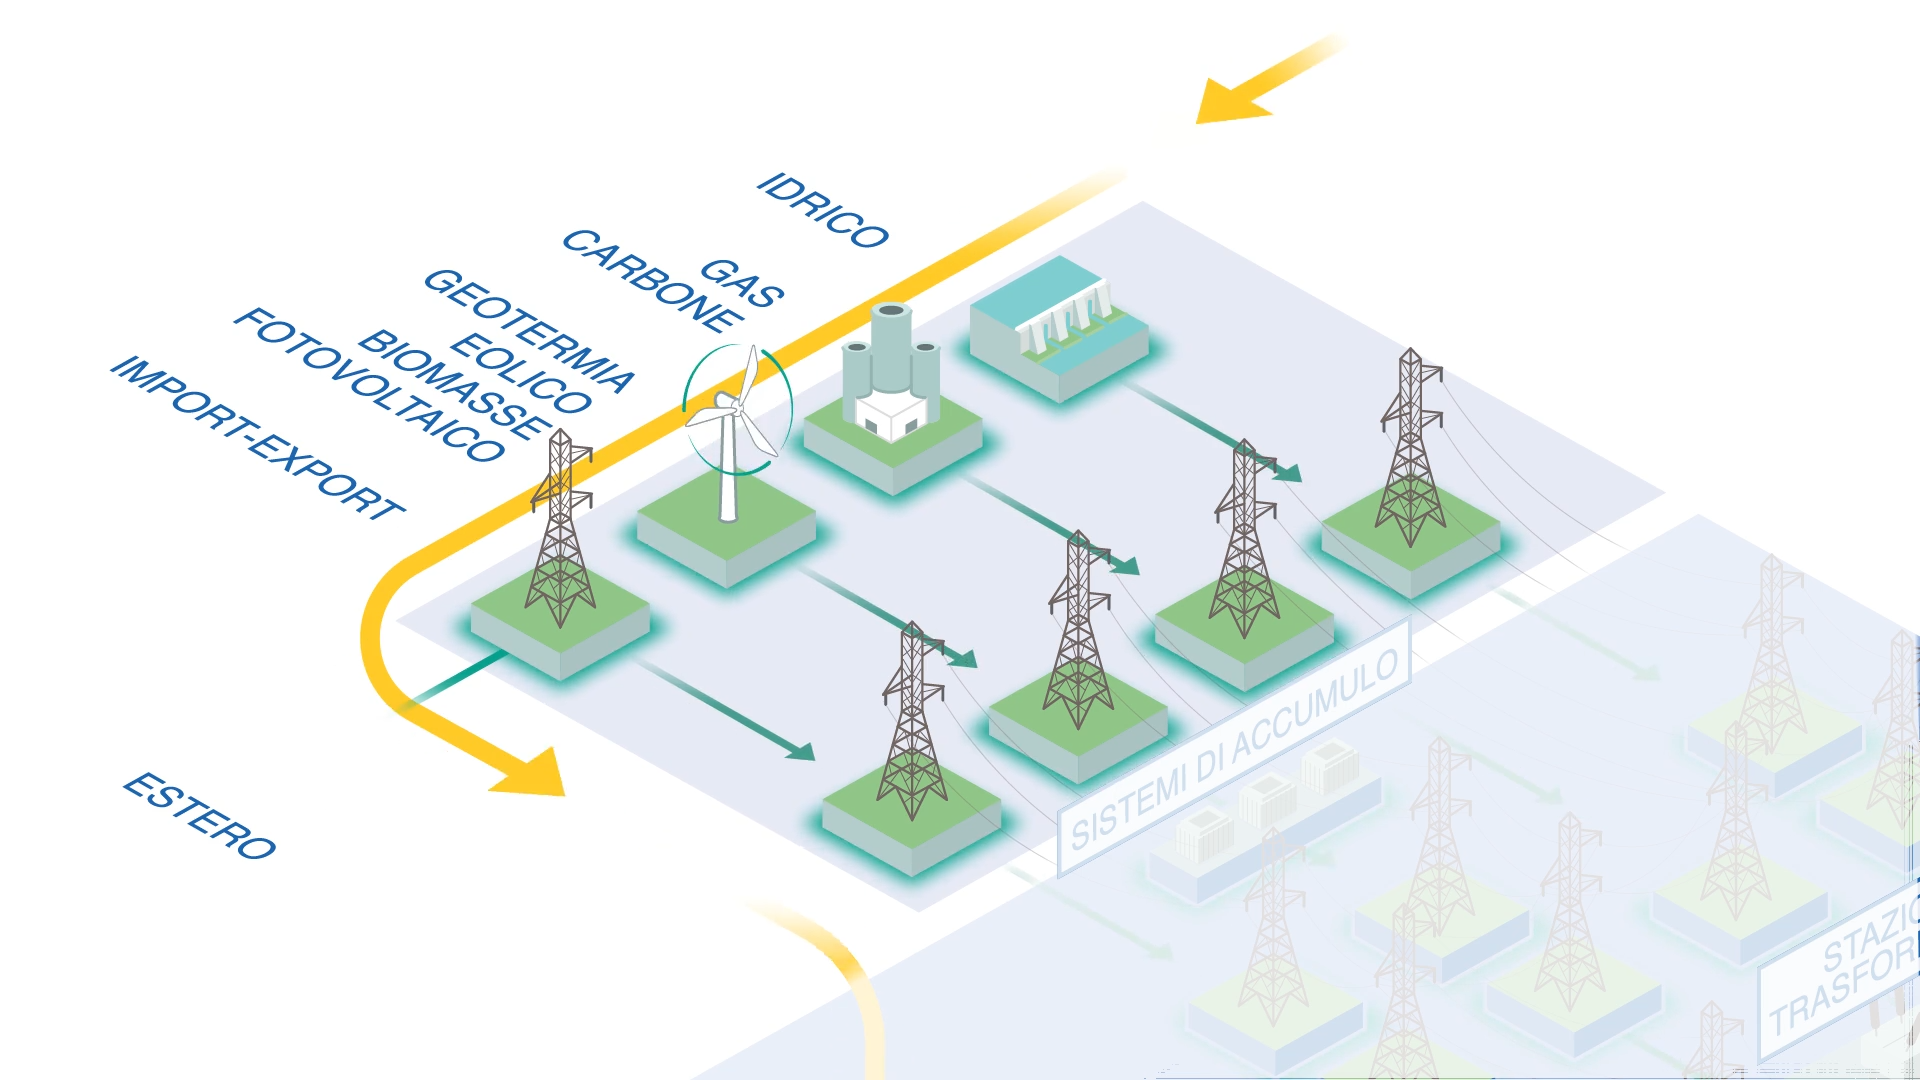
\includegraphics[width=0.9\linewidth]{img/Terna-Produzione.png}
    \caption{Produzione}
\end{figure}

La produzione di elettricità, sia nel sistema tradizionale sia con l'utilizzo delle Smart Grid, avviene attraverso un mix energetico di Fonti Energetiche non Rinnovabili (\textbf{non FER}) e Fonti Energetiche Rinnovabili (\textbf{FER}).

Il mix energetico italiano sfrutta varie fonti tra cui le non FER, con circa il 54\%, e il restante 46\% proviene invece dalle fonti FER Tabella \ref{tab:GSE-mix-nazionale-2023}.


\begin{table}[h!]
    \renewcommand{\arraystretch}{1.2}
    \centering
    \begin{tabular}{c|c}
        % \multicolumn{2}{c}{\shortstack{}}\\
         % \multicolumn{2}{c}{Fonti primarie utilizzate \%} \\
         Fonti primarie utilizzate	& \% \\
         \hline
         Fonti rinnovabili & 46 \\
         Gas naturale& 43 \\
         Carbone& 5 \\
         Altre fonti & 5 \\
         Prodotti petroliferi& 1 \\
    \end{tabular}
    \caption{Composizione del mix iniziale nazionale immessa nel anno 2023 \cite{GSE}}
    \label{tab:GSE-mix-nazionale-2023}
\end{table}



In particolare, come riportato nel "Rapporto Mensile sul Sistema Elettrico 2024" redatto da Terna \cite{TernaRapporto2024}, si mostra che l'assorbimento totale, la somma di produzione più importazioni di energia elettrica, nel periodo Gen-Dic 2024 è stata di $312\,TWh$, di cui FER \footnote{Produzione da FER = Idrico + Biomasse + Geotermico + Eolico + Fotovoltaico} $129\,TWh\,(49\,\%)$, non FER $132\,TWh\ (51\,\%)$ e importazioni $51\,TWh$ principalmente da Francia e Svizzera.

\newpage
\begin{figure}[h!]
    \centering
    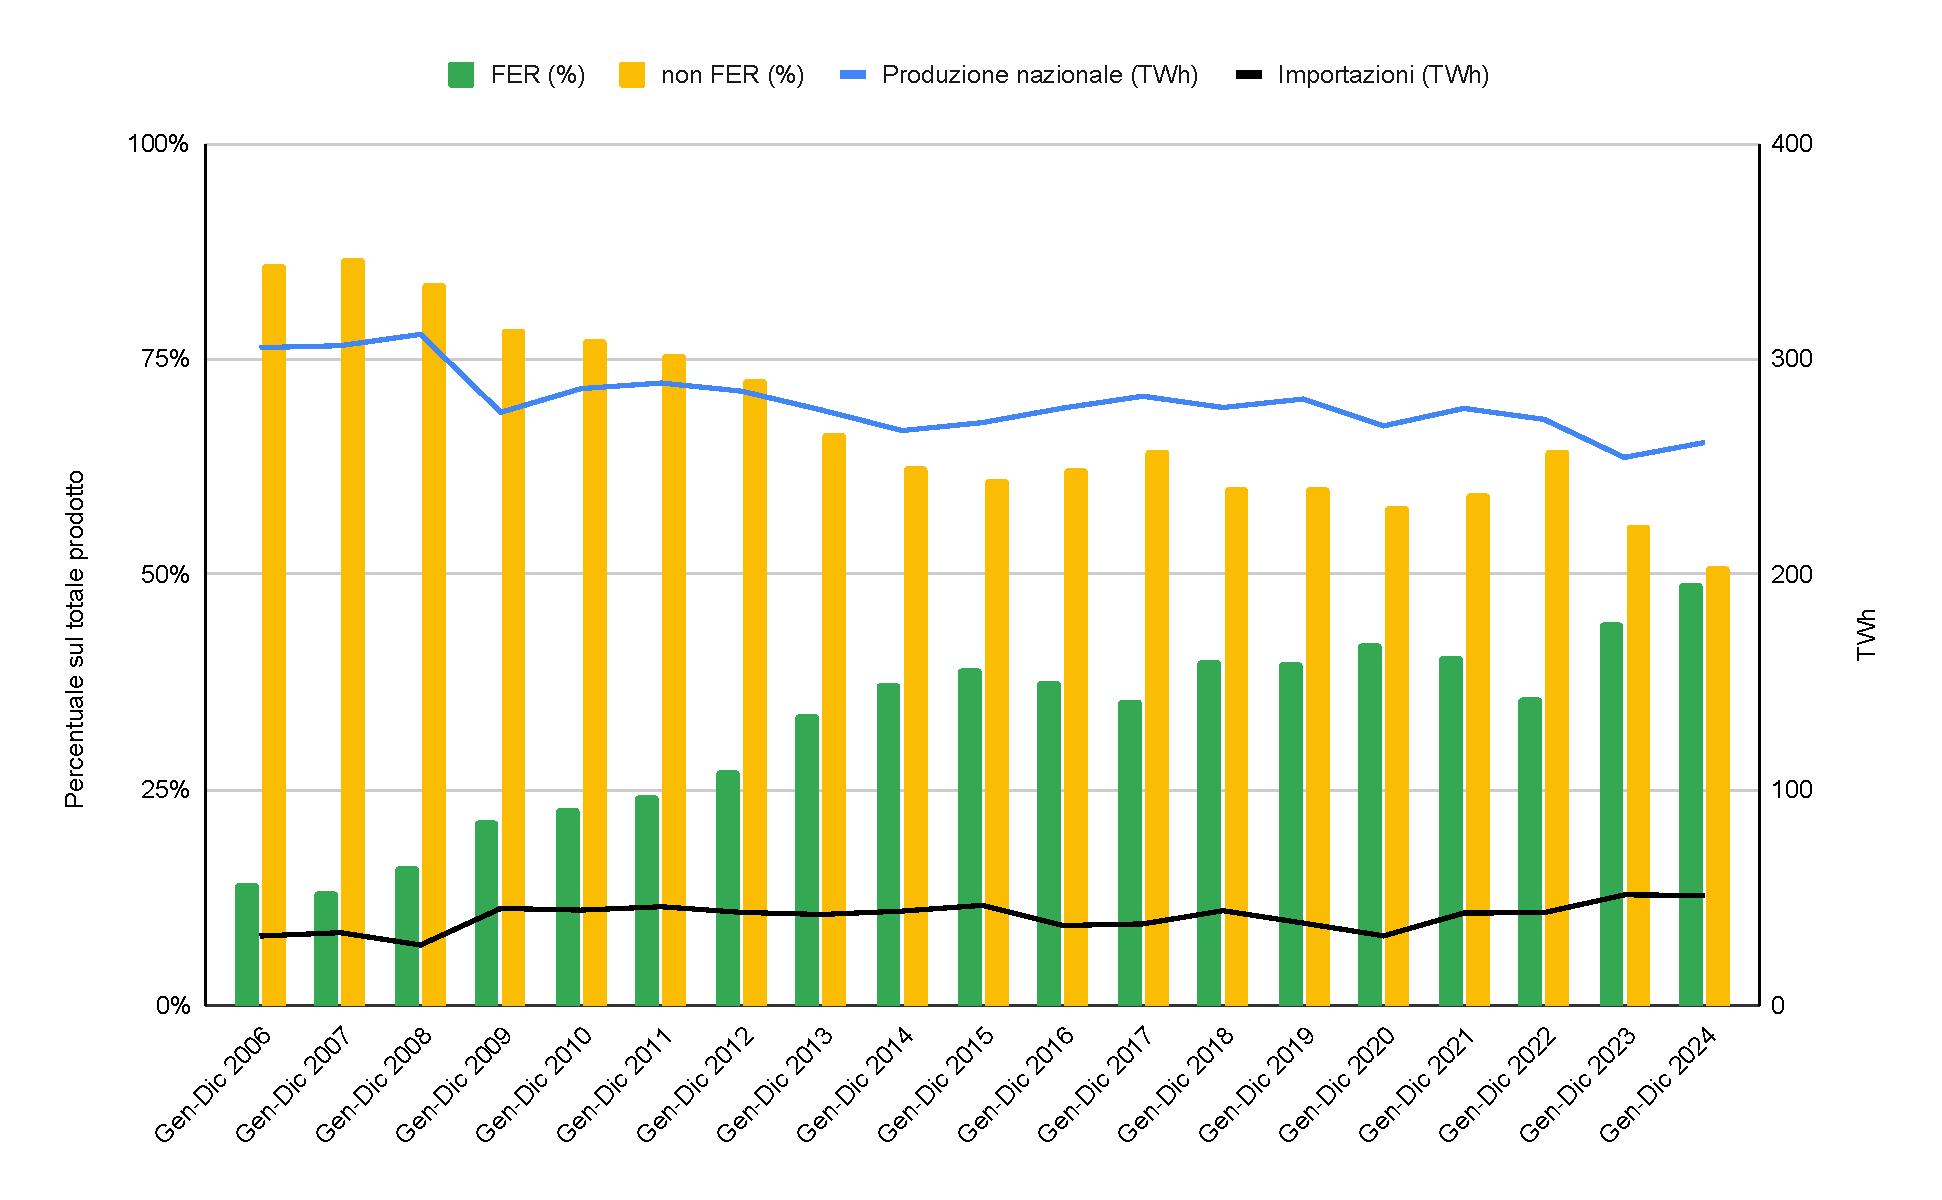
\includegraphics[trim= 1.1cm 0.95cm 1.15cm 1.05cm, clip, width=1\linewidth]{img/Terna-rapporto-annuale-2006-2024.pdf}
    \caption{Produzione nazionale annuale suddivisa tra FER e non FER \cite{terna-rapporto-mensile-sito}}
    \label{graph:Terna-rapporto-annuale-2006-2024}
\end{figure}

Si può vedere dal Grafico \ref{graph:Terna-rapporto-annuale-2006-2024} come dal 2006 al 2024 ci sia stato un incremento consistente della produzione di energia attraverso le fonti FER, arrivando quasi ad un break even nel 2024. In particolar modo, come si evince dal Grafico \ref{graph:Terna-FER-a-confronto-2006-2024}, questa crescita e stata possibile grazie all'installazione di pannelli fotovoltaici a partire dall'anno 2009 e il progressivo e costante aumento degli impani eolici.


\begin{figure}[h!]
    \centering
    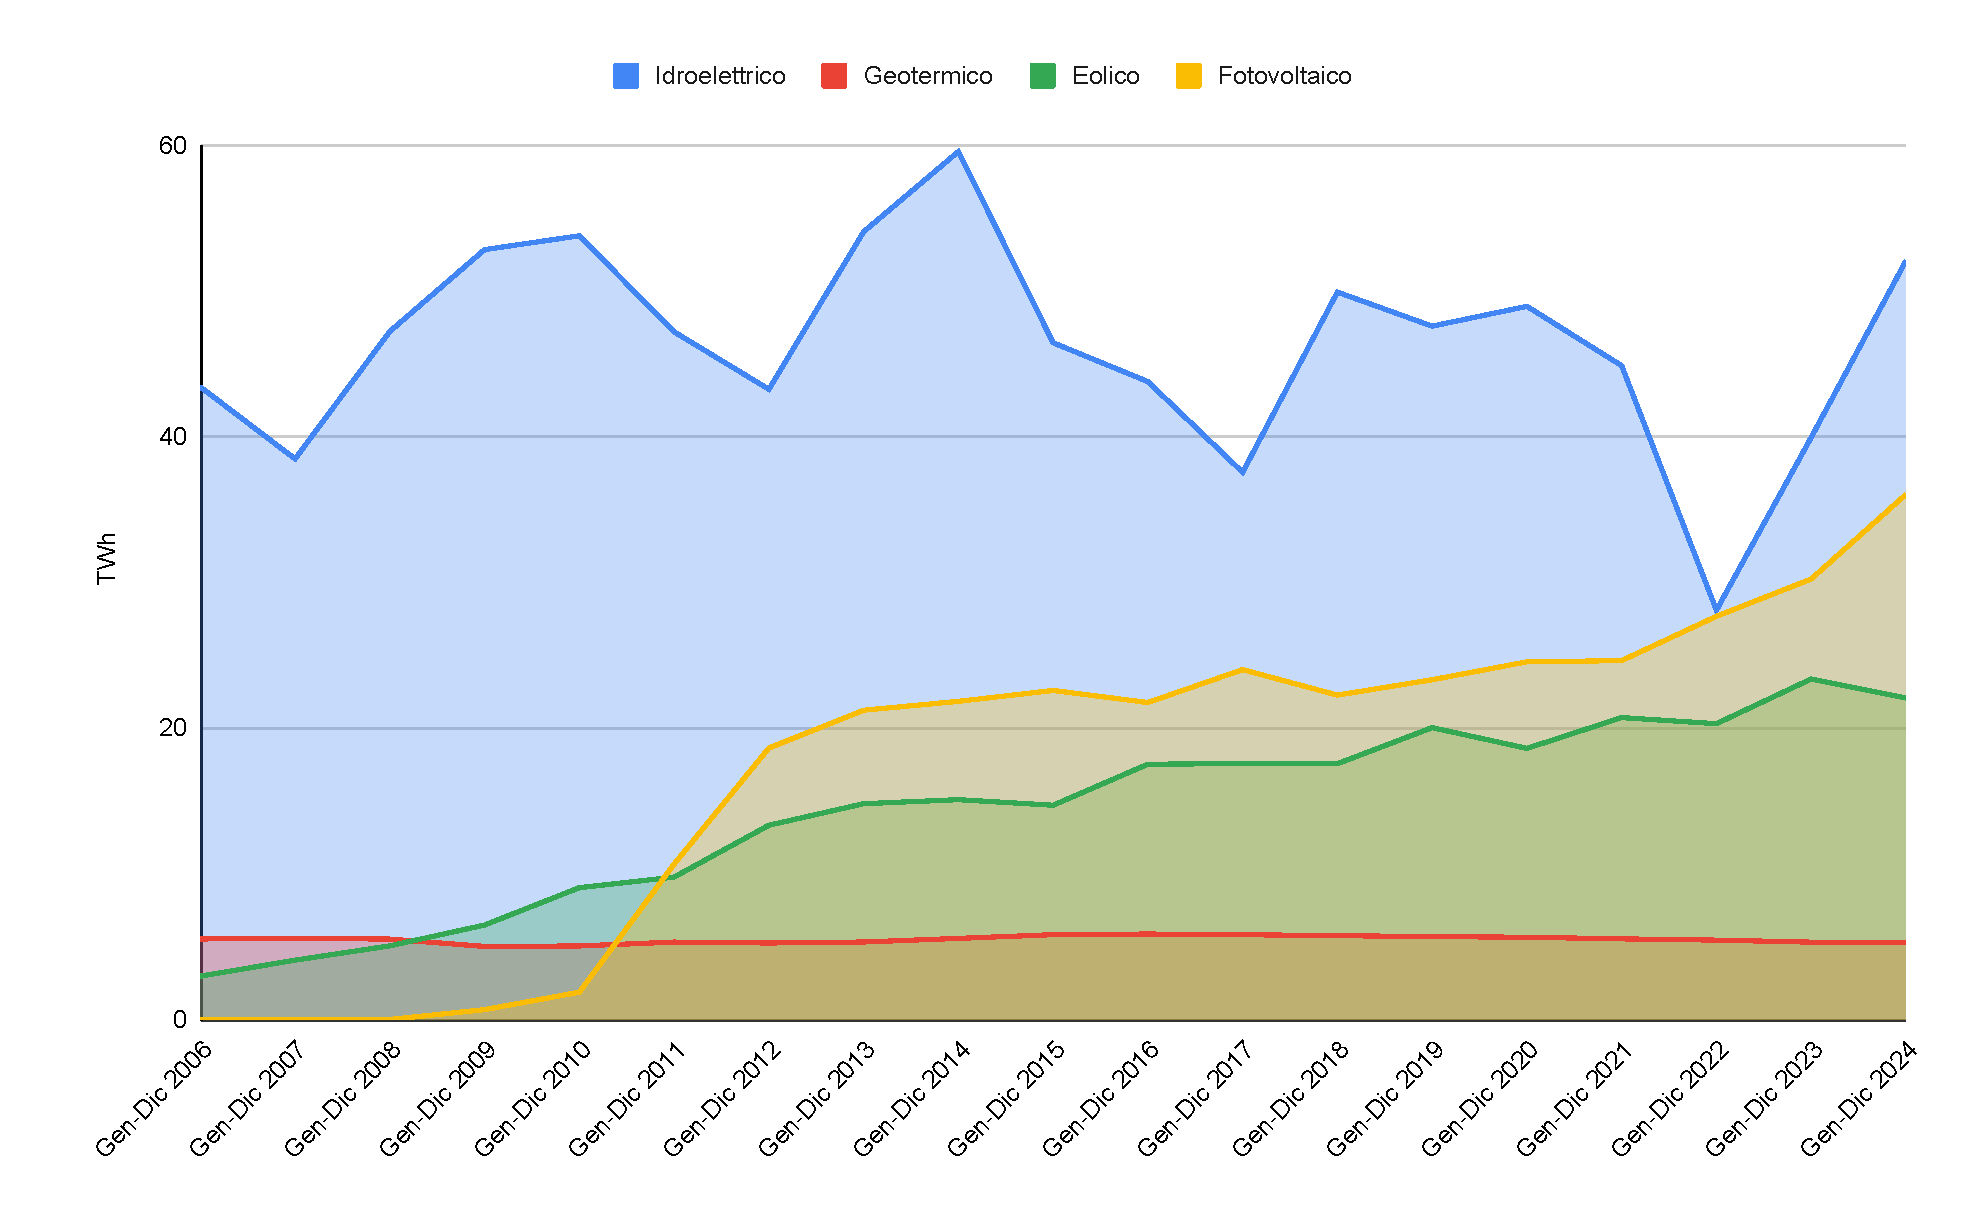
\includegraphics[trim= 1.6cm 1cm 0.85cm 1.05cm, clip, width=1\linewidth]{img/Terna-FER-a-confronto-2006-2024.pdf}
    \caption{Suddivisione delle principali FER in Italia \cite{terna-rapporto-mensile-sito}}
    \label{graph:Terna-FER-a-confronto-2006-2024}
\end{figure}


\subsection{Trasmissione}
La società italiana che, in un regime di monopolio naturale, si occupa della trasmissione e del dispacciamento è Terna. Questa modalità di governance è diffusa anche nel resto d'Europa, poiché è la configurazione ideale da mantenere per garantire una gestione, un mantenimento e uno sviluppo costante su tutta la Rete Elettrica Nazionale (RTN).

La trasmissione è un punto cruciale del dispacciamento dell'energia elettrica che comprende: 

\begin{itemize}
    \item il monitoraggio dei flussi energetici deviando l'energia nelle zone con più alto assorbimento
    \item le disposizioni per gestire l'esercizio coordinato di tutti gli elementi del sistema 
    \item la programmazione di riparazioni, l'allaccio di nuove linee e l'indisponibilità di pezzi della rete
    \item la previsione del fabbisogno energetico nazionale ora per ora
\end{itemize}

Tutto questo tenendo sempre in considerazione che la sinusoide di rete, dalla produzione all'utente finale viene impiegata una corrente alternata, in tutta Italia - ed Europa - deve, in qualsiasi istante, avere un oscillazione di $50\,Hz$, con tolleranza molto bassa nell'ordine di $\pm1\%$, e una tensione di $130\,V$.

\begin{figure}[h!]
    \centering
    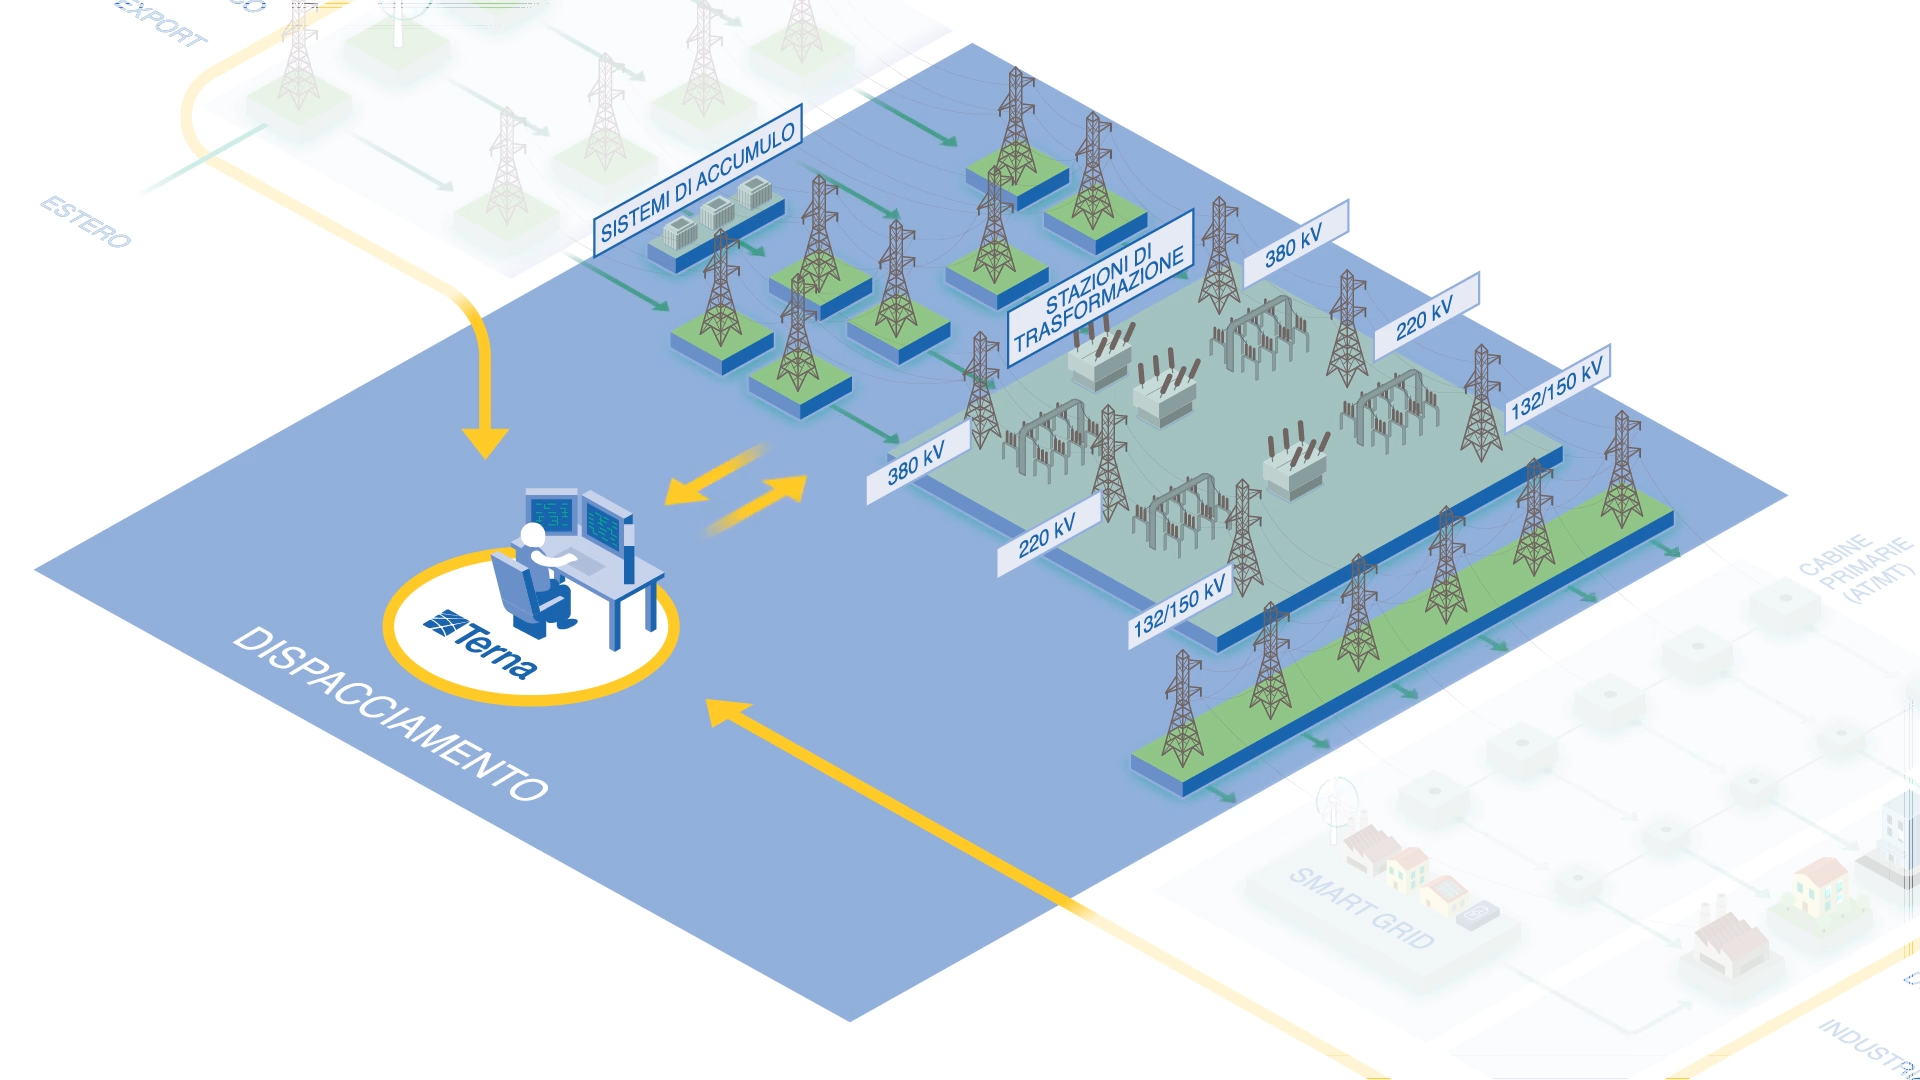
\includegraphics[width=0.9\linewidth]{img/Terna-Trasmissione.png}
    \caption{Trasmissione}
\end{figure}



\newpage
\subsection{Distribuzione}

In Italia, mentre per la trasmissione dell'elettricità, come detto in precedenza, è compito di Terna sulla base della concessione da parte dello Stato, la distribuzione dell'energia elettrica, è gestita da vari soggetti principalmente a livello territoriale.

Attualmente sul territorio nazionale sono $114$ le aziende \cite{arera-distributori} che operano nel settore della distribuzione dell'energia elettrica

Le principali, che servono assieme la quasi totalità dei cittadini dell'intero territorio nazionale sono:

\begin{itemize}
    
    \item E-Distribuzione: società del Gruppo Enel con ben 31.1 milioni di utenti serviti \cite{Clienti-sertivi-distribuzione} su tutto il territorio
    
    \item Areti: società del Gruppo Acea con 2,8 milioni di utenti operante nei territori di Roma e Formello \cite{Clienti-sertivi-areti}
    
    \item Unareti: società del Gruppo A2A con 1,2 milioni di utenti che gestisce i territori di Brescia, Milano e Bergamo \cite{Clienti-sertivi-uniareti}
    
    \item Ireti: società del Gruppo Iren con  700 mila utenti serviti nei territori di Parma, Torino e Vercelli \cite{Clienti-sertivi-ireti}
    
    \item Set Distribuzione: società del Gruppo Dolomiti Energia che serve il territorio della provincia autonoma di Trento con 330 mila utenze servite \cite{Clienti-sertivi-SetDistribuzione}
    
    \item V-reti: società del Gruppo AGSM AIM nata dall'integrazione tra Servizi a Rete (SAR) e Megareti. Sono 279 mila le utenze servite nel territorio di Verona e Vicenza  \cite{Clienti-sertivi-v-reti}
    
    \item Edyna: società del Gruppo Alperia, nata nel 2016 dalla fusione di Azienda EnergeticaReti e SELNET, distribuisce l'energia nel territorio altoatesino servendo 240 mila utenti.\cite{Clienti-sertivi-edyna}
    
    \item InRete: società del Gruppo Hera distribuisce l'energia a oltre 264 mila utenti in Emilia-Romagna e in Toscana  \cite{Clienti-sertivi-edyna}

    
\end{itemize}


Il distributore è responsabile del trasporto, della trasformazione e della consegna ad utenti finali e produttori dell'energia elettrica su reti in Media Tensione, da $1\,kV$ a $35\,kV$, e Bassa Tensione $<1kV$.
L'energia elettrica viene prelevata dalla rete ad Alta Tensione, da $35\,kV$ a $150\,kV$, e portata al livello di Media Tensione  all'interno delle Cabine Primarie.

\begin{figure}[h!]
    \centering
    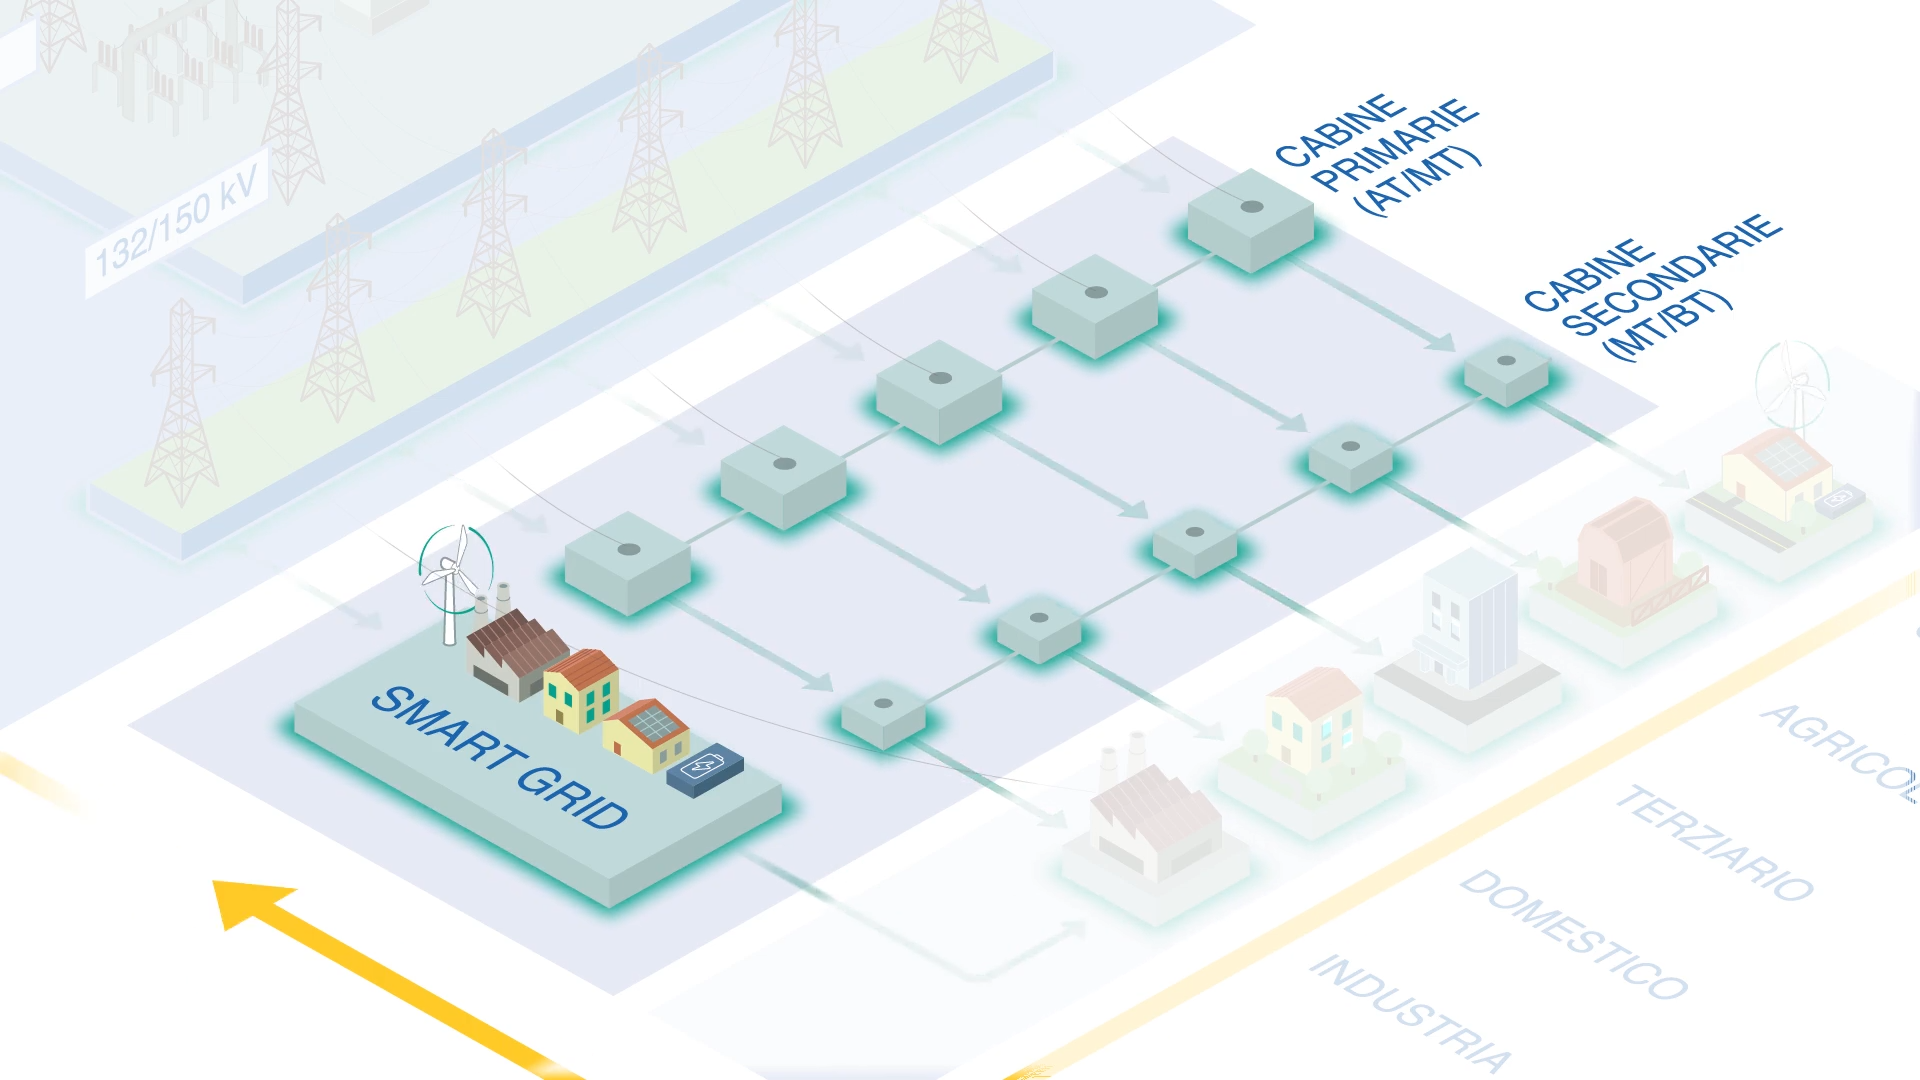
\includegraphics[width=0.9\linewidth]{img/Terna-Distribuzione.png}
    \caption{Distribuzione}
\end{figure}


\newpage
\subsection{Utenze finali}

\begin{figure}[h!]
    \centering
    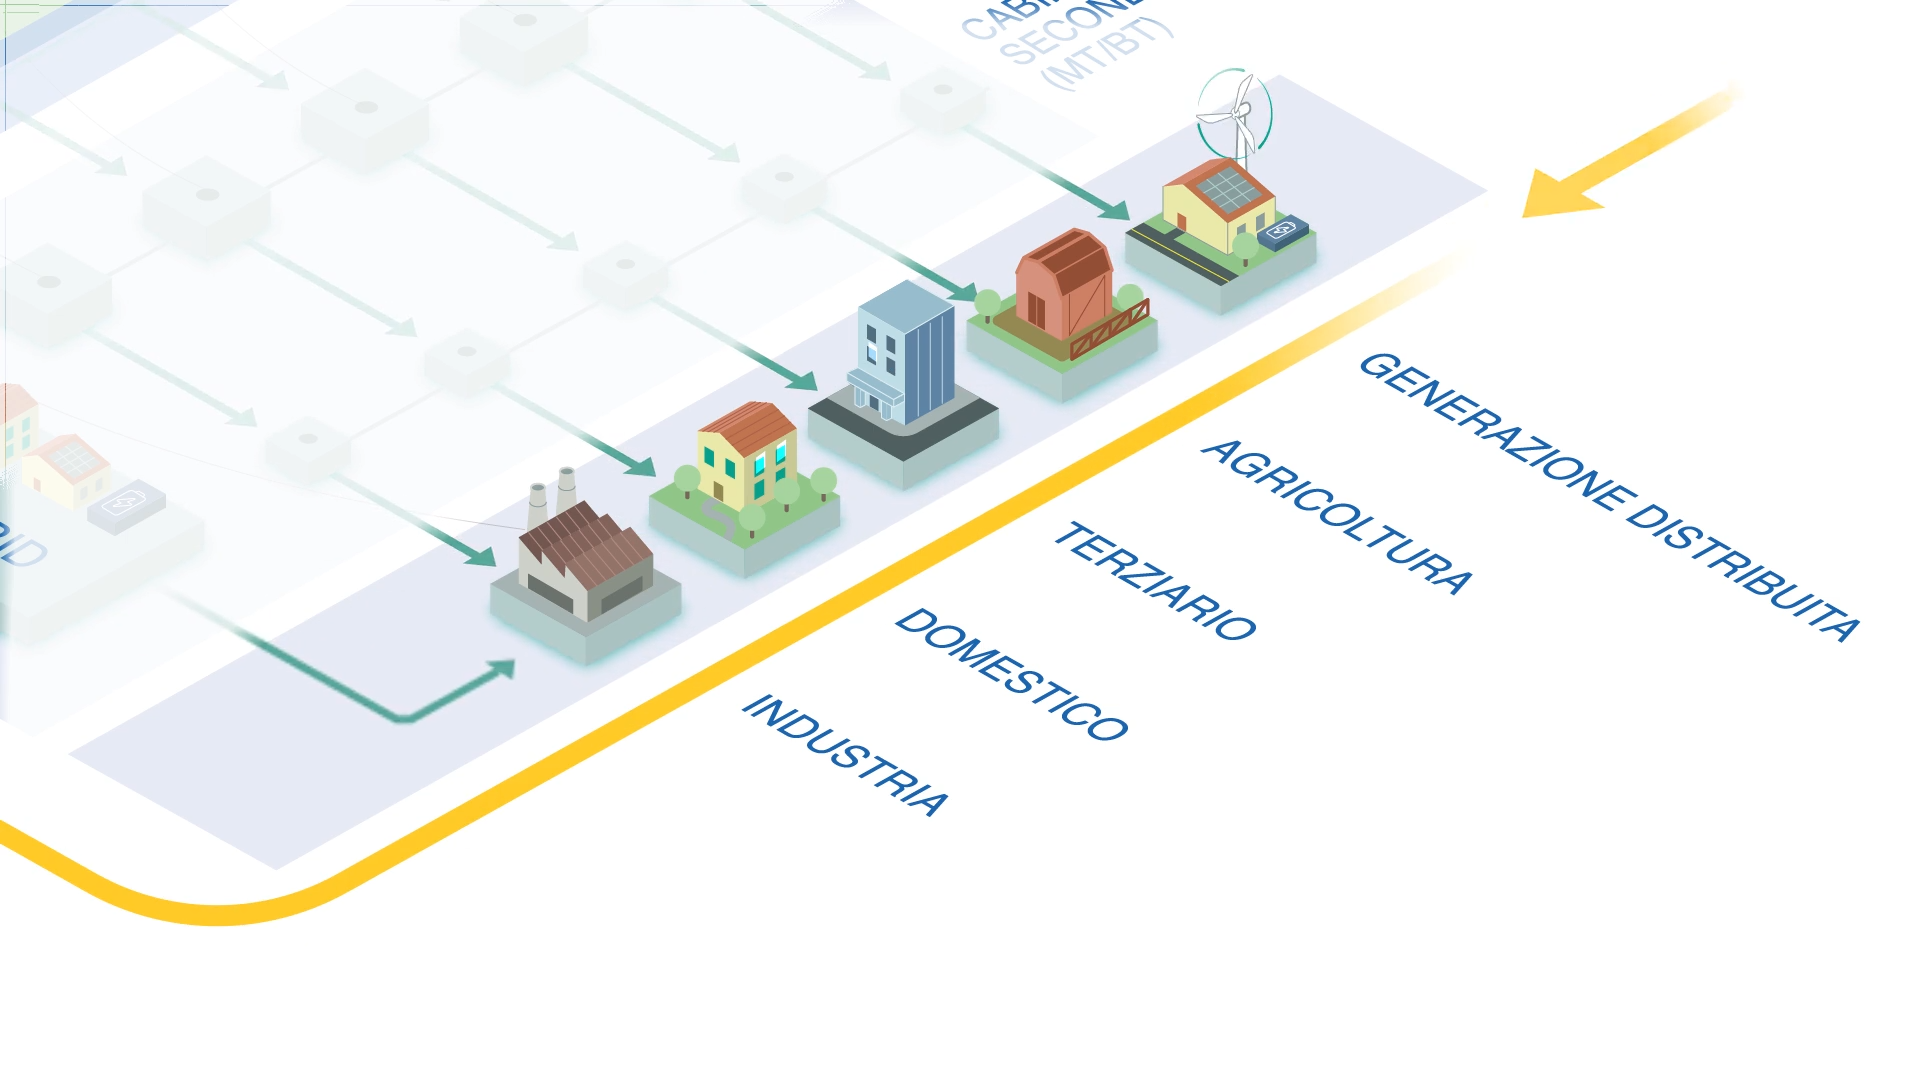
\includegraphics[width=0.9\linewidth]{img/Terna-Utenze.png}
    \caption{Utenze}
\end{figure}


Gli utenti finali possono scegliere il proprio venditore di energia elettrica in base alle specifiche esigenze e alle offerte di mercato.

Molto utile può essere infatti l'utilizzo de \href{https://www.ilportaleofferte.it/portaleOfferte/}{"Il portale delle offerte"} messo a disposizione proprio da ARERA. Questo comparatore fornisce all'utente finale una panoramica chiara di tutte le offerte disponibili sul mercato, questo per poter fare una scelta consapevole.


\section{Componenti principali della Smart Grid}

In questa sezione descriverò i domini relativi al consumatore e al livello più operazionale quale il dominio della trasmissione e distribuzione.

\subsection{Dominio del cliente}

Questo è il dominio più vicino al cliente ed è comporto da:

\begin{itemize}
    \item Smart Meter (\textbf{SM}) 
    \item Home/Building Energy Management Systems (\textbf{HEMS}/BEMS)
    \item Advanced Metering Infrastructure (\textbf{AMI})
\end{itemize}

\subsubsection{Smart Meter}

Gli Smart Meter, o più comunemente chiamati "contatori", sono quei dispositivi che ogni abitazione, negozio e azienda deve avere per allacciarsi alla rete elettrica.
Questo dispositivo conta quanti kWh (chilowattora) sono stati consumati da una specifica utenza e sulla basa di questo il venditore, con cui si ha stipulato il contratto, manderà la fattura da pagare.


Secondo il D. Lgs. 102/2014, che ha recepito la Direttiva Europea 2012/27/UE sull'efficienza energetica, tutti gli smart meter di prima generazione (1G) dovranno essere sostituiti con dei più moderni contatori di seconda generazione (2G) entro il 2035.

E-Distribuzione ha già completato questa transizione a fine del 2024 \cite{sostituzione-contatori-e-dist}, altri, come Ireti, prevedono di sostituirli completamente entro la fine del 2026 \cite{sostituzione-contatori-Ireti}.




      \newpage
\chapter{Smart Grid in ambiente cloudificato}



      \afterpage{\blankpage}
\newpage
% \chapter{Threat Model - Modellazione delle minacce}
% \chapter{Modellazione di minacce informatiche}

% \chapter{Minacce informatiche: analisi, tecniche e identificazione}

\chapter{Modellazione delle Minacce Informatiche: Metodologie e Framework Applicativi}


% who will attack the system, how the
% attack will be deployed, and outlining possible security measures and controls to
% stop the threat before it damages the system.


% Nel capitolo precedente ho introdotto i benefici dell'utilizzo del Cloud Computing, arrivando a presentare una Smart Grid in un contesto Cloud-native decentralizzato con la sua descrizione.

% In questo capitolo invece mi occuperò del fulcro di questa ricerca di tesi, ovvero la modellazioni di minacce informatiche (threat modelling) in questo ambiente Smart Grid cloudificato.

Nel capitolo precedente è stata presentata un'architettura per la Smart Grid basata su un paradigma \textit{Cloud-Native} decentralizzato. È stato dimostrato come tale approccio offra significativi vantaggi in termini di scalabilità, resilienza e agilità. Tuttavia, la transizione da sistemi on-premise a infrastrutture distribuite e basate su cloud altera profondamente il panorama delle minacce, introducendo nuove superfici di attacco e vettori di compromissione.


Pertanto, una valutazione proattiva e sistematica di queste nuove vulnerabilità diventa un'attività indispensabile per garantire la sicurezza e l'affidabilità dell'intera infrastruttura. Questo capitolo costituisce il nucleo metodologico della tesi, fornendo gli strumenti concettuali per la modellazione delle minacce (\textit{Threat Modeling}), un processo strutturato per identificare, analizzare e mitigare i rischi di sicurezza fin dalla fase di progettazione di un sistema.

La trattazione seguirà un percorso logico:
\begin{enumerate}
    \item Inizialmente, verrà definito il processo di \textit{Threat Modeling} e i suoi ambiti applicativi.
    \item Successivamente, verranno illustrati i passi fondamentali che compongono questa metodologia.
    \item Verrà poi introdotto in dettaglio il framework STRIDE, la metodologia scelta per la classificazione sistematica delle minacce in questo studio.
    \item Infine, verranno esaminate le tipologie di minacce specifiche delle architetture \textit{cloud}, preparando il terreno per l'applicazione pratica di questi concetti al modello di Smart Grid proposto nel capitolo successivo.
\end{enumerate}

\section{Esigenze e ambiti applicativi}

% Negli ultimi anni gli attacchi informatici rivolti direttamente ad applicazioni software sono frequenti, causando danni di disponibilità del servizio oltre che a danni economici e finanziari.

% Per limitare che le possibili minacce possano causare danni anche difficilmente riparabili, sempre di più ci si preoccupa di utilizzare delle tecniche di basate sul concetto di \textit{Secure by Design} e l'analisi delle possibili minacce così da prevedere possibili attacchi informatici.

% Di fatto le vulnerabilità all'interno del software sono presenti voi perché introdotte dal team di sviluppo, dalle policy aziendali, dai fornitori, dagli stessi framework o soluzioni open-sorce utilizzate \cite{agid}.

Il panorama della sicurezza informatica è oggi caratterizzato da un'escalation costante di attacchi rivolti alle applicazioni software, con conseguenze che vanno dall'indisponibilità dei servizi a gravi danni economici e reputazionali. Per affrontare questa sfida, l'industria si sta spostando da un approccio puramente reattivo (rispondere agli incidenti dopo che si sono verificati) a un approccio proattivo, basato sul principio del \textit{Secure by Design}.


Questo paradigma impone di integrare la sicurezza in ogni fase del ciclo di vita dello sviluppo del software (SDLC), partendo dal presupposto che le vulnerabilità sono una conseguenza inevitabile della complessità dei sistemi. Le loro origini, infatti, sono molteplici e possono derivare da \cite{agid}: 

\begin{itemize}
    \item Errori di programmazione introdotti dal team di sviluppo.
    \item Debolezze nelle policy di sicurezza aziendali.
    \item Vulnerabilità ereditate da componenti di terze parti, \textit{framework} o librerie \textit{open-source}.
\end{itemize}


In questo contesto, la modellazione delle minacce (\textit{Threat Modeling}) emerge come lo strumento metodologico chiave per implementare il \textit{Secure by Design}. Esso è un processo strutturato che, attraverso l'astrazione e l'analisi del sistema, consente di identificare e ragionare sulle potenziali minacce prima che queste possano essere sfruttate.


L'obiettivo finale del \textit{Threat Modeling} non è solo creare una lista di possibili attacchi, ma fornire le informazioni necessarie per una corretta gestione del rischio. Per ogni minaccia identificata, l'organizzazione può infatti prendere una decisione strategica informata, scegliendo se il rischio debba essere:

\begin{itemize}
    \item \textbf{Mitigato:} applicando una contromisura;
    \item \textbf{Eliminato:} rimuovendo la componente o la funzionalità vulnerabile;
    \item \textbf{Trasferito:} attraverso un'assicurazione o delegando a terzi;
    \item \textbf{Accettato:} se il costo della mitigazione supera il potenziale danno.
\end{itemize}


% L'utilizzo di framework per la ricerca delle minacce che vedremo più avanti permette, attraverso l'astrazione, di aiutare e riflettere su queste vulnerabilità che il sistema, qualsiasi esso sia, possa incorrere e scegliere se la vulnerabilità debba essere: \textbf{Mitigata}, \textbf{Eliminata}, \textbf{Trasferita} o semplicemente \textbf{Accettata}.



\section{Il Processo di Threat Modeling}


"\textit{La modellazione delle minacce è un \textbf{processo strategico}\footnote{Si riferisce alla capacità di anticipare le minacce attraverso modelli di attacco simulati.} volto a prendere in considerazione i possibili scenari di  \textbf{attacchi} e \textbf{vulnerabilità} all'interno di un ambiente applicativo proposto o esistente allo scopo di identificare chiaramente i livelli di \textbf{rischio} e di \textbf{impatto}.}" \cite{libro-threat-modelling}

% \vspace{0.3cm}

L'adozione di questa metodologia offre vantaggi tangibili durante tutto il ciclo di vita dello sviluppo \cite{libro-threat-modelling-designin-for-security}:


% \begin{itemize}
%     \item Consente di individuare possibili bug\footnote{Un bug è un errore nel codice di un programma che causa malfunzionamenti o comportamenti inaspettati, e può rappresentare una vulnerabilità sfruttabile per attacchi informatici.} nelle fasi iniziali dello sviluppo software, cruciale per risparmiare risorse rispetto a trovarlo nelle fasi finali o nel prodotto finito;
%     \item Consente di capire meglio i requisiti di sicurezza, soprattutto considerare i requisiti non presi in considerazione;
%     \item Permette di progettare e consegnare un prodotto migliore, evitando la necessità di riprogettare il sistema;
%     \item Permette di affrontare problemi che altre tecnologie non possono affrontare.
% \end{itemize}


\begin{itemize}
    \item \textbf{Identificazione Precoce dei Difetti:} Permette di individuare vulnerabilità di progettazione nelle fasi iniziali dello sviluppo, riducendo drasticamente i costi di correzione rispetto a un loro rilevamento in fasi successive o dopo il rilascio del prodotto;
    \item \textbf{Definizione dei Requisiti di Sicurezza:} Aiuta a chiarire e a completare i requisiti di sicurezza, evidenziando aspetti inizialmente non considerati;
    \item \textbf{Miglioramento della Progettazione:} Conduce a un'architettura più robusta e sicura, minimizzando la necessità di costose riprogettazioni;
    \item \textbf{Analisi dei Rischi Logici:} A differenza di strumenti automatici che trovano bug\footnote{Un bug è un errore nel codice di un programma che causa malfunzionamenti o comportamenti inaspettati, e può rappresentare una vulnerabilità sfruttabile per attacchi informatici.} nel codice, il \textit{Threat Modeling} è in grado di identificare difetti logici e di progettazione che nessun'altra tecnologia può rilevare;
\end{itemize}

Sebbene il processo possa avvalersi di tecniche collaborative come il \textit{brainstorming}, esso viene tipicamente guidato da uno dei seguenti approcci metodologici  \cite{libro-threat-modelling-designin-for-security}:

% \begin{itemize}
%     \item \textbf{Asset-focused:} consiste nello stilare una lista di asset per poi considerare quali possono essere le minacce che possono subire. 
%     % Possibili attacchi possono essere: 
%     % \begin{itemize}
%     % \item[--] cose che un attaccante vuole come password o secret key
%     % \item[--] cose che si vogliono proteggere come la reputazione di un azienda
%     % \item[--] tutti gli asset già identificati possono essere attaccati e
%     % \item[--] sfruttati per raggiungere altri asset.
%     % \end{itemize}
%     \item \textbf{Attacker-focused:} consiste nello stilare una lista dei possibili attaccanti e cercare di immedesimarsi in loro per capire come il sistema può essere minacciato. Questo approccio è rischioso, perché i programmatori possono proiettare le loro conoscenze nel modellare come si comporterebbe un aggressore, creando un modello che non riflette le possibili minacce reali
%     \item \textbf{Software-focused:} è l'approccio più efficiente. Gli sviluppatori, che hanno la massima conoscenza del software che si sta costruendo, partecipano attivamente per aiutare a creando un modello, di solito attraverso diagrammi, del software e identificando possibili bug.
% \end{itemize}

\begin{enumerate}
    \item \textbf{Approccio Centrato sugli Asset (\textit{Asset-centric}):} Il processo inizia con l'identificazione e la classificazione degli asset critici del sistema (es. dati sensibili, funzionalità chiave). Successivamente, si analizzano le minacce che potrebbero compromettere ciascun asset.
    \item \textbf{Approccio Centrato sull'Attaccante (\textit{Attacker-centric}):} Questo approccio si concentra sulla profilazione dei potenziali attaccanti, analizzandone le motivazioni, le capacità e gli obiettivi. Si cerca quindi di simulare le loro possibili azioni contro il sistema. Sebbene utile, questo metodo presenta il rischio che il team di sviluppo proietti le proprie conoscenze e i propri bias nel modello, sottostimando o ignorando le reali tattiche degli avversari.
    \item \textbf{Approccio Centrato sul Software (\textit{Software-centric}):} Considerato spesso il più efficace in contesti di sviluppo, questo approccio parte da una rappresentazione del sistema stesso, tipicamente attraverso diagrammi di flusso dei dati (DFD). Analizzando come i dati si muovono attraverso i componenti del sistema e superano i confini di fiducia (\textit{trust boundaries}), il team può identificare sistematicamente le potenziali vulnerabilità.
\end{enumerate}

\section{Le Fasi del Processo di Threat Modeling}

% Il processo di modellazione delle minacce risponde a quattro domande essenziali \cite{libro-threat-modelling-designin-for-security,agid}:

% \begin{itemize}
%     \item \textbf{Cosa si sta costruendo?} Capire l'architettura di sistema, componenti, flussi di dati e interazioni.
%     \item \textbf{Cosa può andare storto una volta costruito?} Trovare le potenziali minacce e vulnerabilità che potrà compromettere la sicurezza di sistema, esaminare con cura i possibili attacchi
%     \item \textbf{Che cosa fare per le cose che possono andare storte?} Sviluppo di strategie e contromisure per controllare e/o minimizzare i rischi
%     \item \textbf{Si è fatto un lavoro di analisi decente?} Step di validazione, testi la tua strategia di mitigazione
% \end{itemize}

% Queste domande prevedono un approccio in quattro fasi:

% \begin{center}
%     Modellare il sistema $\rightarrow$ Trovare le minacce $\rightarrow$ Affrontare le minacce $\rightarrow$ Validare il modello
% \end{center}


Il processo di modellazione delle minacce (\textit{Threat Modeling}) è un'attività iterativa che può essere scomposta in quattro fasi fondamentali. Ciascuna fase è progettata per rispondere a una domanda chiave, guidando il team di analisi dalla comprensione del sistema alla validazione delle contromisure implementate \cite{libro-threat-modelling-designin-for-security,agid}.

Di seguito vengono introdotte le quattro fasi, che saranno analizzate in dettaglio nei paragrafi successivi.

\begin{enumerate}
    \item \textbf{Modellazione del Sistema (Risponde a: "Cosa stiamo costruendo?")}\\ La prima fase consiste nel comprendere e rappresentare formalmente il sistema oggetto di analisi. Questo implica la definizione dei suoi componenti, dei confini di fiducia (\textit{trust boundaries}), delle interfacce e, soprattutto, dei flussi di dati (DFD). Un modello accurato è il prerequisito fondamentale per una corretta identificazione delle minacce.
    \item \textbf{Identificazione delle Minacce (Risponde a: "Cosa potrebbe andare storto?")}\\Una volta definito il modello, la seconda fase si concentra sull'identificazione sistematica delle potenziali minacce. Utilizzando framework strutturati come STRIDE, si analizza ogni elemento del modello per enumerare le vulnerabilità che potrebbero comprometterne la sicurezza. L'obiettivo è creare un elenco completo di possibili scenari di attacco.
    \item \textbf{Mitigazione delle Minacce (Risponde a: "Cosa possiamo fare al riguardo?")}\\In questa fase, per ogni minaccia identificata, si definisce una strategia di gestione del rischio. Ciò comporta la progettazione e la prioritizzazione di contromisure di sicurezza (mitigazioni) volte a ridurre la probabilità o l'impatto della minaccia. Le strategie possono includere la modifica della progettazione, l'implementazione di controlli di sicurezza o la revisione delle policy.
    \item \textbf{Validazione delle Mitigazioni (Risponde a: "Abbiamo fatto un buon lavoro?")}\\La fase finale chiude il ciclo verificando che le minacce siano state adeguatamente affrontate. Questo include la revisione delle contromisure implementate, l'esecuzione di test di sicurezza per validarne l'efficacia e l'aggiornamento della documentazione. Questo step garantisce che il processo abbia effettivamente ridotto il livello di rischio del sistema.
\end{enumerate}



\begin{figure}[!h]
    \centering
    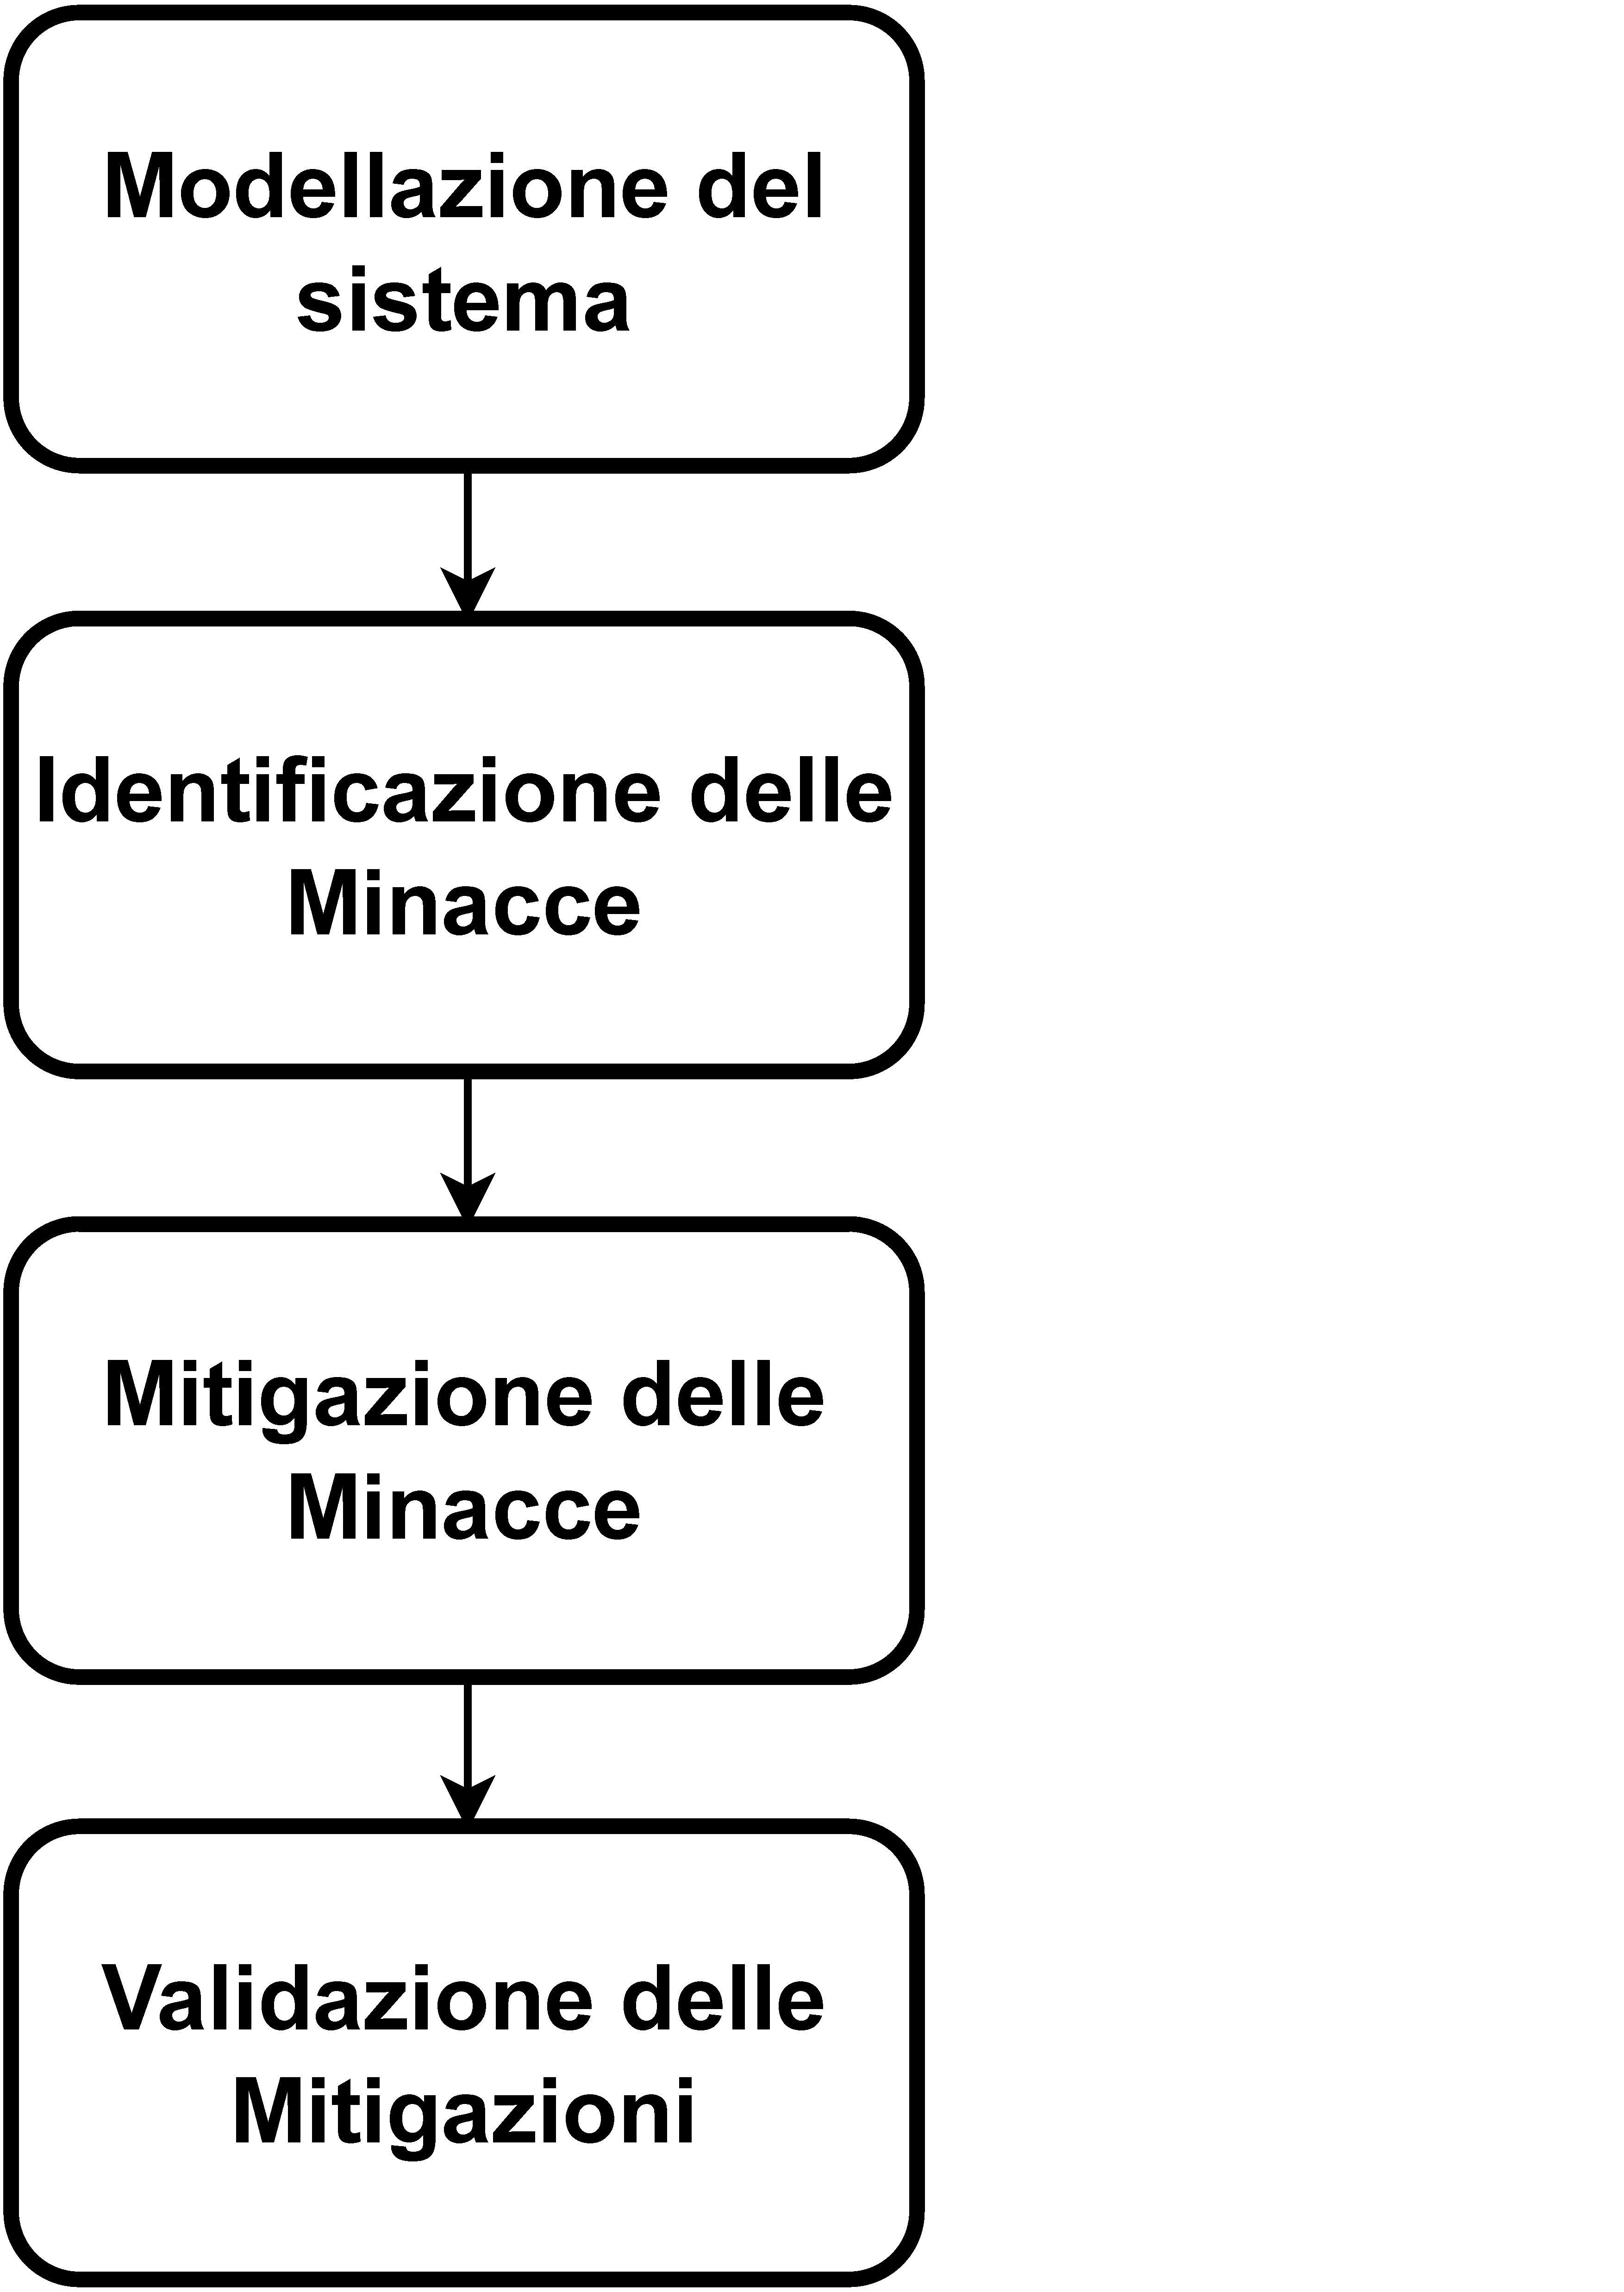
\includegraphics[trim= 0cm 0cm 25.5cm 0cm, clip, width=0.15\linewidth]{img/the-4-step-framework-v2.drawio.pdf}
    \caption{Le Fasi del Processo di Threat Modeling}
    \label{fig:4-step-framework}
\end{figure}



\subsection{Modellazione del sistema}

% Il primo passo è quello di capire il sistema nel suo complesso. Questo può essere fatto attraverso una decomposizione, un processo che permette di acquisire conoscenze su come funziona il sistema e come interagisce con le entità esterne. 

% La decomposizione include:

% \begin{itemize}
%     \item la creazione di \textit{casi d'uso - use case}, per identificare le modalità di utilizzo del sistema;
%     \item l'identificazione dei \textit{punti di ingresso - entry points}, che permettono a un aggressore di interagire con il sistema;
%     \item l'identificazione degli \textit{asset} a cui un attaccante potrebbe essere interessato;
%     \item la scoperta di \textit{attori}, utenti che interagiscono con il sistema; essi possono essere interni o esterni e devono ricevere alcuni diritti di accesso;
%     \item l'identificazione dei \textit{livelli di fiducia - trust boundaries}, che determineranno i diritti di accesso per entità esterne.
% \end{itemize}

% Una delle tecniche per decomporre il sistema è la creazione di un Data Flow Diagram (DFD). Questo tipo di diagramma è stato introdotto negli anni '70 per dare una rappresentazione visiva del modo in cui i dati si spostano da un componente all'altro in un sistema o di un'applicazione e dove i dati vengono modificati o memorizzati (temporaneamente o a lungo termine) all'interno del sistema.

% La DFD identifica chiaramente le \textit{Entità esterne}, i \textit{Punti finali} del sistema, i \textit{processi},e le \textit{unità di funzione}, il \textit{Data Flow} (DF) e il \textit{Data Store} (DS).
% Più tardi, nei primi anni 2000, è stato aggiunto il concetto di \textit{trust boundaries}\footnote{ Un trust boundaries definisce il punto dove cambia il livello di fiducia tra due componenti o domini di un sistema} per migliorare le DFD.
% I trust boundaries vengono utilizzati per isolare gli elementi attendibili e non attendibili. \cite{STRIDE-paper}


La prima e fondamentale fase del processo di \textit{Threat Modeling} consiste nel creare una rappresentazione astratta ma accurata del sistema da analizzare. L'obiettivo è comprendere a fondo i suoi componenti, le interazioni e, soprattutto, come i dati fluiscono e vengono trattati al suo interno.


Lo strumento standard per questa attività è il \textit{Data Flow Diagram} (DFD). Introdotto originariamente negli anni '70, il DFD è una tecnica di rappresentazione grafica che visualizza il flusso di informazioni all'interno di un sistema. Invece di mostrare la logica di controllo (come farebbe un \textit{flowchart}), un DFD si concentra esclusivamente sul movimento e sulla trasformazione dei dati.


Un DFD è composto da quattro elementi fondamentali:


\begin{enumerate}
    \item \textbf{Entità Esterne (\textit{External Entities}):} Rappresentano gli attori, sia umani che altri sistemi, che interagiscono con il sistema inviando o ricevendo dati, ma che si trovano al di fuori del suo controllo (es. un utente, un'API di terze parti).
    \item \textbf{Processi (\textit{Processes}):} Sono le componenti del sistema che elaborano o trasformano i dati. Ogni processo prende dei dati in input e produce dei dati in output.
    \item \textbf{Archivio dati (\textit{Data Store}):} Rappresentano i luoghi in cui i dati vengono archiviati, sia in modo temporaneo (es. una cache) che permanente (es. un database).
    \item \textbf{Flussi di Dati (Data Flows):} Sono le frecce che collegano gli altri elementi del diagramma, indicando la direzione in cui i dati si muovono.
\end{enumerate}

Per l'analisi di sicurezza, i DFD sono stati arricchiti con un quinto elemento cruciale: i Confini di Fiducia (\textit{Trust Boundaries}). Questi confini sono linee tratteggiate che delimitano le aree del sistema con diversi livelli di privilegio o fiducia. Un flusso di dati che attraversa un trust boundary rappresenta un punto di ingresso critico (\textit{entry point}) e una potenziale superficie di attacco che richiede un'analisi particolarmente attenta \cite{STRIDE-paper}.


La costruzione di un DFD costringe il team a rispondere a domande essenziali: quali sono gli asset da proteggere? Chi sono gli attori che interagiscono con il sistema? Quali sono i punti di ingresso e come vengono validati i dati che li attraversano? Questo modello diventa così la mappa su cui, nella fase successiva, verranno sistematicamente identificate le minacce.



\subsection{Identificazione  delle minacce}

% Questo è l'elemento centrale della modellazione delle minacce: le minacce e gli agenti di minaccia\footnote{Agente di minaccia: individuo o gruppo interessato a sfruttare una vulnerabilità e a realizzare un'azione di
% minaccia contro l'asset} possono essere essere identificati seguendo diversi diverse metodologie: 

% \begin{itemize}
%     \item STRIDE
%     \item Attack threes
%     \item PASTA
%     \item CVSS
%     \item Security Cards.
% \end{itemize}

% Per lo scopo di questa tesi verrà utilizzata la prima metodologia: STRIDE.

Una volta ottenuto un modello chiaro del sistema attraverso il DFD, la seconda fase del processo consiste nell'identificare sistematicamente le minacce. Questa attività, spesso definita "\textit{threat enumeration}", ha lo scopo di rispondere alla domanda: "Cosa potrebbe andare storto?". Si analizza ogni componente del DFD (processi, flussi di dati, data store) per individuare le potenziali vulnerabilità.


Per guidare questa analisi in modo strutturato e ripetibile, sono stati sviluppati numerosi framework e metodologie. Tra i più noti si includono:


\begin{itemize}
    \item \textbf{STRIDE:} Un modello di classificazione delle minacce sviluppato da Microsoft, focalizzato sulle proprietà di sicurezza che un software dovrebbe garantire.
    \item \textbf{Attack Trees: }Una tecnica che scompone un potenziale attacco in una struttura ad albero, mappando i passaggi necessari per raggiungere un obiettivo malevolo.
    \item \textbf{PASTA (\textit{Process for Attack Simulation and Threat Analysis}):} Una metodologia completa in sette fasi che allinea le minacce agli obiettivi di business.
    \item \textbf{CVSS (\textit{Common Vulnerability Scoring Syste}m):} Sebbene non sia una metodologia di \textit{threat modeling}, è un sistema di punteggio utilizzato per valutare la gravità delle vulnerabilità una volta identificate.
    \item \textbf{LINDDUN:} Un framework specifico per l'identificazione di minacce alla privacy.
\end{itemize}


Per l'analisi condotta in questa tesi, è stato scelto il framework STRIDE. Questa decisione è motivata dalla sua stretta integrazione con la modellazione basata su DFD e dalla sua efficacia nell'identificare un'ampia gamma di minacce a livello di progettazione software. La sua natura sistematica lo rende particolarmente adatto ad analizzare sistemi complessi e distribuiti come l'architettura Smart Grid \textit{Cloud-Native} proposta. Il framework STRIDE verrà descritto in dettaglio nella sezione seguente.


\subsection{Mitigazione delle Minacce}

% Una volta identificate le minacce, è necessario comprendere come affrontarle, quali sono più urgenti da gestire e quali contromisure di sicurezza sono necessarie per mitigare il loro impatto. Una tecnica utile è creare una matrice di tracciabilità delle minacce: gli attacchi vengono elencati sulla base del pericolo ad essi associato. Tenendo conto del livello di rischio associato a ciascuna vulnerabilità durante il processo di gestione del rischio, le minacce vengono classificate da più gravi a meno gravi, e le parti interessate e i proprietari del rischio possono analizzarle per trovare le contromisure appropriate e le tecniche di mitigazione. I rischi verranno trattati secondo quanto definito nel processo di gestione del rischio.

Una volta completata l'identificazione delle minacce, la terza fase del processo si concentra su come affrontarle. Non è sufficiente avere una lista di potenziali attacchi; è necessario valutarli, prioritizzarli e definire contromisure adeguate. Questo processo si articola in tre attività principali.

% \vspace{-0.11cm}
\begin{enumerate}
    \item \textbf{Valutazione del Rischio (Risk Assessment):}
    Per ogni minaccia identificata, viene effettuata una valutazione del rischio associato. Questo non si basa solo sulla natura della minaccia stessa, ma su una combinazione di due fattori chiave:
    % \vspace{-0.11cm}
    \begin{itemize}
        \item \textbf{Probabilità (\textit{Likelihood}):} La probabilità che la vulnerabilità possa essere effettivamente sfruttata da un attaccante.
        \item \textbf{Impatto (\textit{Impact}):} Il danno potenziale (operativo, finanziario, reputazionale) che si verificherebbe in caso di successo dell'attacco.
    \end{itemize}
    % \vspace{-0.11cm}
     Molte metodologie, come DREAD, assegnano un punteggio a questi fattori per calcolare un livello di rischio complessivo per ogni minaccia.
     % \vspace{-0.11cm}
    \item \textbf{Prioritizzazione delle Minacce:}
    Sulla base del livello di rischio calcolato, le minacce vengono classificate in ordine di priorità, da quelle più critiche a quelle meno gravi. Questo permette al team di concentrare le risorse e l'attenzione sulla risoluzione dei problemi che rappresentano il maggior pericolo per il sistema.
    % \vspace{-0.11cm}
    \item \textbf{Definizione delle Contromisure:}
    Per le minacce prioritarie, si passa alla progettazione delle contromisure (o mitigazioni). L'obiettivo è applicare controlli di sicurezza che riducano la probabilità o l'impatto della minaccia a un livello accettabile. Come già discusso nel contesto della gestione del rischio, le opzioni non si limitano alla mitigazione; il team può decidere di eliminare una funzionalità, trasferire il rischio o accettarlo consapevolmente.
\end{enumerate}

% \vspace{-0.11cm}

% Per documentare questo processo, si utilizza spesso una matrice di tracciabilità delle minacce, che associa a ogni minaccia identificata il suo livello di rischio, la contromisura proposta e lo stato di implementazione, garantendo che nessuna vulnerabilità nota venga trascurata.


\subsection{Validazione delle Mitigazioni}


% Quest'ultimo passaggio consiste nel verificare se il modello di minaccia è completo (se identifica tutte le possibili minacce) e se tutte le minacce sono adeguatamente mitigate. Per le minacce che non sono state completamente mitigate, il rischio residuo viene calcolato e analizzato (il rischio residuo è coerente con il livello di rischio accettabile?).[13] Una strategia comune per validare il modello di minaccia è l'utilizzo di test. I test possono essere automatici o manuali e possono essere applicate diverse tecniche. Ad esempio, il penetration testing può essere utilizzato per valutare le vulnerabilità del sistema (le vulnerabilità trovate vengono confrontate con quelle identificate dal modello di minaccia), oppure le tecniche di mitigazione identificate dal modello vengono validate simulando un attacco e applicando quelle tecniche per verificare se sono realmente in grado di mitigare l'attacco.

La fase finale del processo di Threat Modeling chiude il ciclo, assicurando che il lavoro svolto abbia effettivamente migliorato la postura di sicurezza del sistema. Questa fase di validazione ha un duplice obiettivo: verificare la completezza dell'analisi e l'efficacia delle contromisure implementate. Le attività principali includono:

% \vspace{-0.11cm}
\begin{enumerate}
    \item \textbf{Revisione del Modello e delle Contromisure:}
    Si riesamina l'intero modello di minaccia per confermarne l'accuratezza e la completezza. Il team si assicura che tutte le minacce identificate siano state associate a una strategia di gestione del rischio e che le contromisure progettate siano state implementate correttamente secondo le specifiche.
    % \vspace{-0.11cm}
    \item \textbf{Analisi del Rischio Residuo:}
    È raro che tutte le minacce possano essere eliminate completamente. Per le minacce che sono state mitigate (ma non eliminate) o accettate, si valuta il rischio residuo, ovvero il livello di rischio che permane nel sistema dopo l'applicazione dei controlli di sicurezza. È compito dei responsabili del rischio (\textit{risk owner}) determinare se tale rischio residuo rientri nella soglia di tolleranza definita dall'organizzazione.
    % \vspace{-0.11cm}
    \item \textbf{Test di Sicurezza e Validazione Pratica:}
    Per verificare empiricamente l'efficacia delle mitigazioni, si ricorre a test di sicurezza. Questi possono includere:
    % \vspace{-0.11cm}
    \begin{itemize}
        \item \textbf{\textit{Penetration Testing}:} Viene eseguito un attacco simulato da parte di "\textit{ethical hacker}" per tentare di sfruttare le vulnerabilità del sistema. I risultati vengono poi confrontati con le minacce identificate nel modello per verificarne la copertura.
        \item \textbf{\textit{Security Test Case}:} Vengono creati casi di test specifici per validare che ogni singola contromisura funzioni come previsto (es. "verificare che un input malizioso venga correttamente rigettato dal sistema di validazione").
    \end{itemize}
\end{enumerate}
% \vspace{-0.11cm}

Solo al termine di questa fase di validazione si può considerare concluso un ciclo di \textit{Threat Modeling}. Il modello, tuttavia, non è un documento statico: deve essere rivisto e aggiornato ogni volta che il sistema subisce modifiche significative.

\section{Il framework utilizzato: STRIDE}

% È stato creato da Microsoft per tre scopi principali \cite{STRIDE-paper}: 

% \begin{enumerate}
%     \item come approccio sistematico per analizzare le possibili minacce informatiche contro ogni componente del sistema basandosi sulla sua conoscenza tecnica;
%     \item per fornire un'analisi completa delle proprietà di sicurezza;
%     \item per identificare l'impatto della vulnerabilità di un componente sull'intero sistema.
% \end{enumerate}

% STRIDE è l'acronimo per il tipo di minacce che copre \cite{libro-threat-modelling-designin-for-security}:

% \begin{itemize}
%     \item \textbf{Spoofing:} violazione della proprietà di autenticazione. L'attaccante finge di essere qualcun altro, come un processo, un'entità esterna o una persona e compromette qualcosa all'interno del sistema. Uno scenario comune può essere: l'attaccante sfrutta un sistema di autenticazione debole (ad esempio, intercettando la chiave da API che utilizzano richieste di autenticazione a chiave singola). Una volta rubata la chiave e ottenuto l'accesso al sistema, l'attaccante finge di essere un processo innocuo e crea o modifica maliziosamente un file prima del processo reale.
%     \item \textbf{Tampering:} violazione della proprietà di integrità. L'attaccante modifica qualcosa (un file, il codice o alcuni dati) in modo non autorizzato. Questo attacco potrebbe essere rilevato controllando i file di log e le notifiche.
%     \item \textbf{Repudiation:} violazione della proprietà di non ripudio. Garantisce che un comportamento scorretto non possa essere provato. Alcuni meccanismi di non ripudio potrebbero essere l'auditing e il tracciamento (ma considerando sempre che anche i file di tracciamento potrebbero essere manomessi).
%     \item \textbf{Information disclosure:} violazione della proprietà di riservatezza. Alcune informazioni riservate potrebbero essere accidentalmente divulgate (ad esempio, attraverso messaggi di errore) o essere esposte a un attacco (come il buffer overflow).
%     \item \textbf{Denial of Service (DoS):} violazione della proprietà di disponibilità. Un sistema diventa irraggiungibile sfruttando maliziosamente le sue risorse e impedendogli di essere utilizzato per scopi legittimi. Alcuni esempi possono essere DoS che colpiscono i processi (l'attacco assorbe memoria o CPU e il processo non è in grado di funzionare) o database (vengono riempiti con informazioni inutili e non sono in grado di ricevere dati utili).
%     \item \textbf{Elevation of privilege:} violazione della proprietà di autorizzazione. L'attaccante dichiara di essere un utente autorizzato con privilegi elevati (come admin invece di un utente comune). Ad esempio, corrompendo un processo, l'attaccante può ottenere diritti di accesso in lettura o scrittura a alcune posizioni di memoria sensibili.
% \end{itemize}


% Una volta creato il DFD, la modellazione delle minacce basata su STRIDE può essere eseguita in due modi: 

% \begin{itemize}
%     \item STRIDE per-elemento: per ogni minaccia coperta da STRIDE, ogni componente del sistema viene analizzato per verificare se può essere soggetto a questa minaccia.
%     \item STRIDE-per-interazione: i componenti del sistema sono considerati in tuple (origine, destinazione e interazione) e la loro interazione viene analizzata per verificare se può essere soggetta a una o più minacce coperte da STRIDE.
% \end{itemize}

Sviluppato originariamente da Microsoft, STRIDE è un modello di classificazione delle minacce che aiuta gli analisti a identificare sistematicamente un'ampia gamma di vulnerabilità di sicurezza. Il suo scopo è fornire un approccio mnemonico e strutturato per ragionare sulle possibili minacce contro ogni componente di un sistema, mappando ogni minaccia a una specifica proprietà di sicurezza che viene violata \cite{STRIDE-paper, libro-threat-modelling-designin-for-security}.

L'acronimo STRIDE rappresenta sei categorie di minacce:
\begin{itemize}
    \item \textit{\textbf{S}poofin}g (Falsificazione dell'identità): Si verifica quando un aggressore si finge illegittimamente un altro utente, componente o sistema. Viola la proprietà di Autenticazione.
    % * Esempio: Un attaccante ruba le credenziali di un utente e accede al sistema impersonandolo, oppure un processo malevolo si finge un processo legittimo per ricevere dati sensibili.
    \item \textit{\textbf{T}ampering} (Manomissione): Consiste nella modifica non autorizzata di dati, sia in transito su una rete che archiviati in un data store. Viola la proprietà di Integrità.
    % * Esempio: Un attaccante intercetta un flusso di dati e ne altera il contenuto, oppure modifica direttamente un file di configurazione o un record in un database.
    \item \textit{\textbf{R}epudiation} (Ripudio): Si riferisce alla capacità di un utente di negare di aver compiuto un'azione, in assenza di prove che dimostrino il contrario. Viola la proprietà di Non Ripudio.
     % * Esempio: Un utente esegue un'operazione dannosa e poi cancella i file di log per eliminare le tracce, rendendo impossibile attribuirgli l'azione.
    \item \textit{\textbf{I}nformation Disclosure} (Rivelazione di informazioni): Consiste nell'esposizione di informazioni sensibili a soggetti non autorizzati. Viola la proprietà di Confidenzialità.
    % * Esempio: Un messaggio di errore che rivela dettagli interni del sistema, un accesso non autorizzato a un database, o una vulnerabilità come un buffer overflow che espone dati in memoria.
    \item \textit{\textbf{D}enial of Service} (DoS - Negazione del servizio): Si verifica quando un attaccante rende un sistema o una risorsa non disponibile per gli utenti legittimi. Viola la proprietà di Disponibilità.
    % * Esempio: Un attacco che esaurisce la CPU o la memoria di un processo, o che inonda una rete di traffico inutile per renderla inaccessibile.
    \item \textit{\textbf{E}levation of Privilege} (EoP - Acquisizione di privilegi): Avviene quando un utente con privilegi limitati riesce a ottenere accessi o permessi superiori a quelli che gli sono stati assegnati. Viola la proprietà di Autorizzazione.
    % * Esempio: Un utente standard sfrutta una vulnerabilità per ottenere i privilegi di amministratore, ottenendo così accesso a funzionalità e dati riservati.
\end{itemize}

La forza di STRIDE risiede nella sua applicazione sistematica a un \textit{Data Flow Diagram}.
Una volta creato il DFD, la modellazione delle minacce basata su STRIDE può essere eseguita in due modi: 

\begin{itemize}
    \item STRIDE per-elemento: per ogni minaccia coperta da STRIDE, ogni componente del sistema viene analizzato per verificare se può essere soggetto a questa minaccia.
    \item STRIDE-per-interazione: i componenti del sistema sono considerati in tuple (origine, destinazione e interazione) e la loro interazione viene analizzata per verificare se può essere soggetta a una o più minacce coperte da STRIDE.
\end{itemize}

% \section{Minacce informatiche su architettura cloud}

% \newpage
% \chapter{Applicazione del Threat Modeling all'Architettura Proposta}

% % \section{Applicazione del Threat Modeling: Modellazione del Sistema}


% % Giunti a questo punto, dopo aver analizzato i passi da seguire per modellizzare le minacce possiamo iniziare con il definire il Data Flow Diagram del nostro sistema Smart Grid.

% % \begin{figure}[!h]
% %     \centering
% %     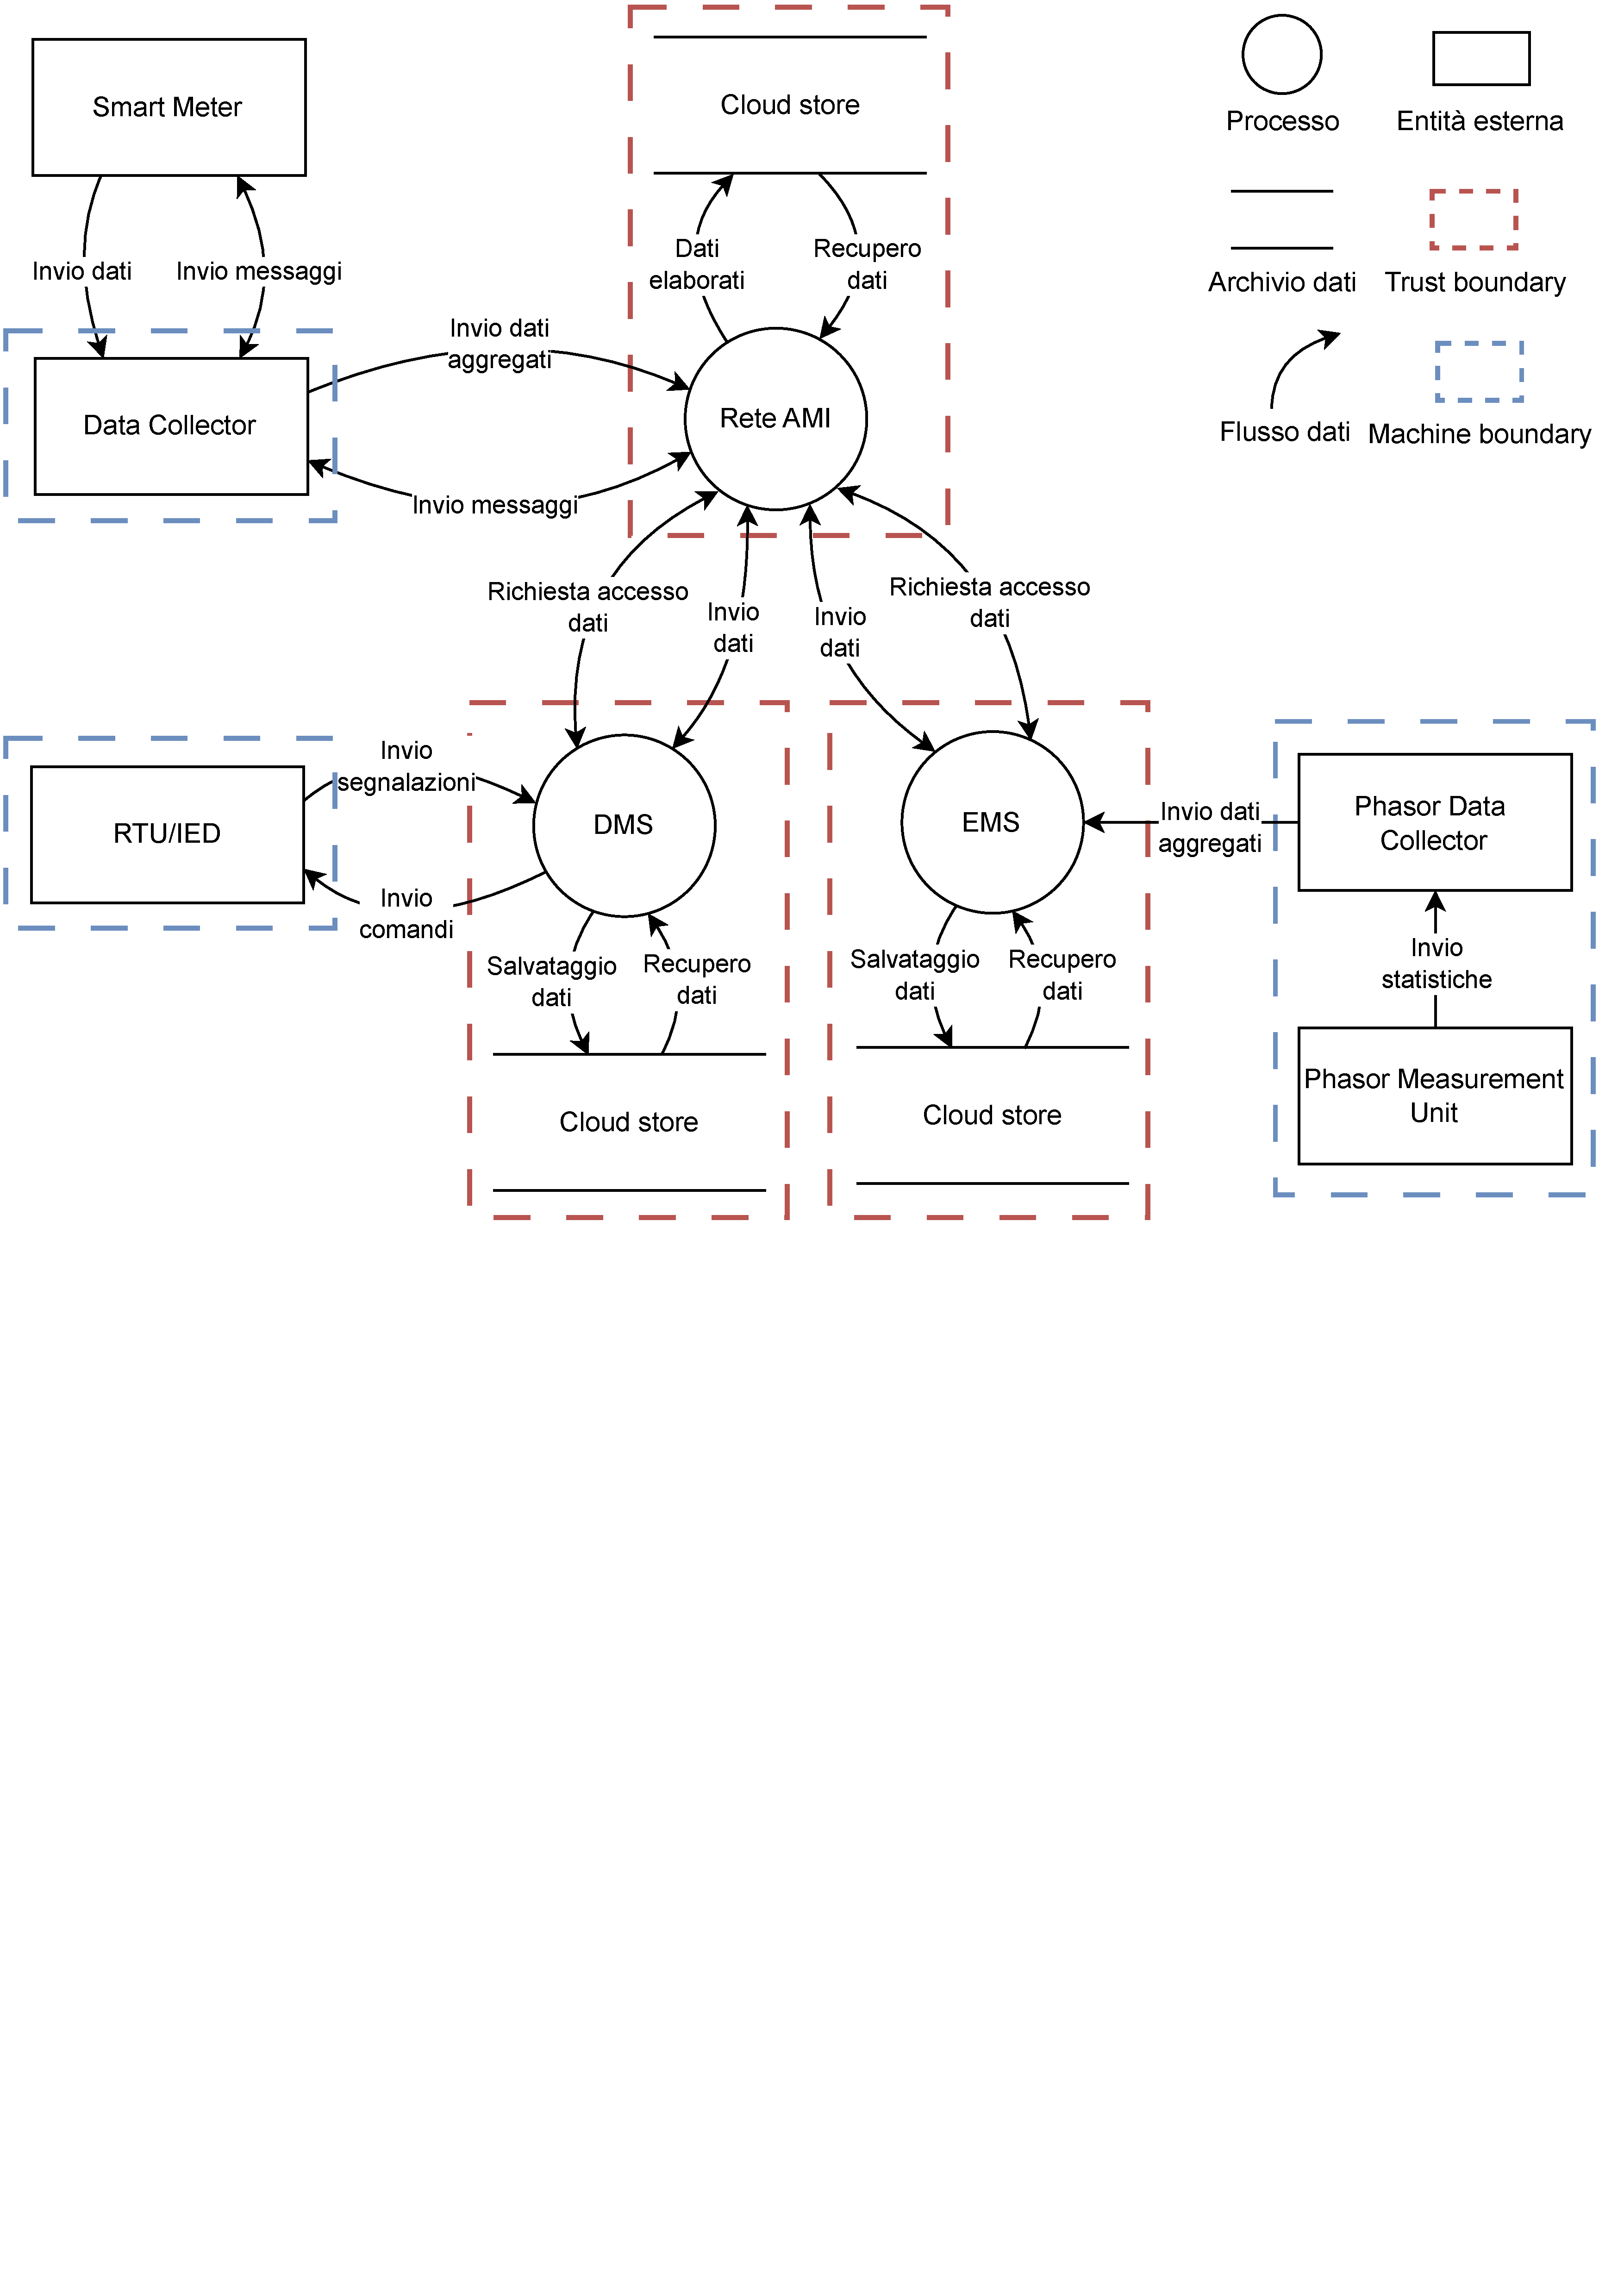
\includegraphics[trim= 0cm 39cm 0cm 0cm, clip, width=0.8\linewidth]{img/DFD.drawio.pdf}
% %     \caption{Data flow diagram - Smart Grid Cloud-Native}
% %     \label{fig:DFD}
% % \end{figure}

% % Come si vede dalla Figura \ref{fig:DFD}, visione semplificata delle componenti cardine, sono stati identificati dei \textit{Boundaries}, ovvero dei confini sicuri, che possono essere di due tipologie:

% % \begin{itemize}

% %     \item Trust Boundaries (rossi): generici confini di sicurezza, garantiti di fatto dalla presenta dell'architettura Cloud-Native.
% %     \item Machine Boundaries (blu): questi sono dei confini di sicurezza fisici, che proteggono i componenti sul campo da possibili manomissioni.
% % \end{itemize}

% Nei capitoli precedenti sono stati definiti i tre pilastri concettuali di questa tesi: il concetto di Smart Grid con la sua architettura e componenti (Capitolo 1), un'implementazione di una Smart Grid basata su un paradigma Cloud-Native (Capitolo 2) e la metodologia formale del Threat Modeling per l'analisi della sicurezza dei sistemi (Capitolo 3).

% Questo capitolo rappresenta il punto di convergenza di questi tre elementi, costituendo il contributo centrale della ricerca. L'obiettivo è applicare sistematicamente il processo di Threat Modeling, e in particolare il framework STRIDE, al modello architetturale proposto, al fine di identificare e classificare le principali minacce informatiche che lo caratterizzano.


% L'analisi seguirà fedelmente le quattro fasi metodologiche descritte in precedenza:

% \begin{enumerate}
%     \item \textbf{Modellazione del Sistema:} Verrà presentato e discusso in dettaglio il Data Flow Diagram (DFD) dell'architettura.
%     \item \textbf{Identificazione delle Minacce:} Ogni componente del DFD verrà analizzato attraverso la lente di STRIDE per enumerare le potenziali minacce.
%     \item \textbf{Mitigazione delle Minacce:} Per le minacce più significative, verranno proposte delle contromisure di sicurezza specifiche per il contesto Cloud-Native.
%     \item \textbf{Validazione:} Verranno discusse le strategie per la validazione delle mitigazioni proposte.
% \end{enumerate}


% % \section{Modellazione del Sistema}
% \section{Definizione del Data Flow Diagram dell'Architettura}

% In questa sezione si avvia l'applicazione pratica del processo di Threat Modeling all'architettura Smart Grid Cloud-Native proposta. Il primo passo fondamentale, come descritto dalla metodologia, consiste nella modellazione del sistema attraverso un Data Flow Diagram (DFD).

% La  Figura \ref{fig:DFD} presenta un DFD di Livello 0 che astrae l'architettura, evidenziandone i componenti principali, i flussi di dati e, soprattutto, i confini di sicurezza. In questo modello sono stati identificati i seguenti elementi:

% \begin{itemize}
%     \item \textbf{Entità Esterne:} Componenti che interagiscono con il sistema ma si trovano al di fuori del suo controllo diretto, come lo Smart Meter, l'RTU/IED e il sistema PMU/Phasor Data Concentrator.
%     \item \textbf{Processi:} I componenti software che elaborano i dati, come il Data Concentrator, la Rete AMI (che agisce come hub di comunicazione), il DMS e l'EMS.
%     \item \textbf{Archivi Dati:} I luoghi di memorizzazione dei dati, rappresentati dai Cloud Store.
% \end{itemize}

% Per l'analisi di sicurezza, sono stati definiti due tipi di confini (boundaries), ciascuno con un significato preciso:

% \begin{enumerate}
%     \item \textbf{Trust Boundary (confine rosso):} Rappresenta un confine logico che separa componenti con diversi livelli di fiducia. Qualsiasi flusso di dati che attraversa un Trust Boundary (ad esempio, dalla "Rete AMI" al processo "DMS") deve essere considerato potenzialmente ostile e quindi soggetto a rigorose procedure di autenticazione, autorizzazione e validazione. Questi confini definiscono la superficie di attacco di ciascun servizio.
%     \item \textbf{Machine Boundary (confine blu):} Rappresenta un confine fisico o a livello di dispositivo. Esso isola i componenti che operano sul campo (Edge), come il Data Concentrator o il Phasor Data Concentrator, dal loro ambiente fisico e dalla rete locale. Questo confine è rilevante per analizzare minacce di accesso fisico (manomissione) o attacchi diretti al dispositivo, che bypasserebbero i controlli a livello di applicazione.
% \end{enumerate}

% % Questo DFD, con la sua chiara distinzione tra processi, dati e confini, costituisce la mappa fondamentale su cui, nella fase successiva, verranno sistematicamente identificate le minacce utilizzando il framework STRIDE.



% \begin{figure}[!h]
%     \centering
%     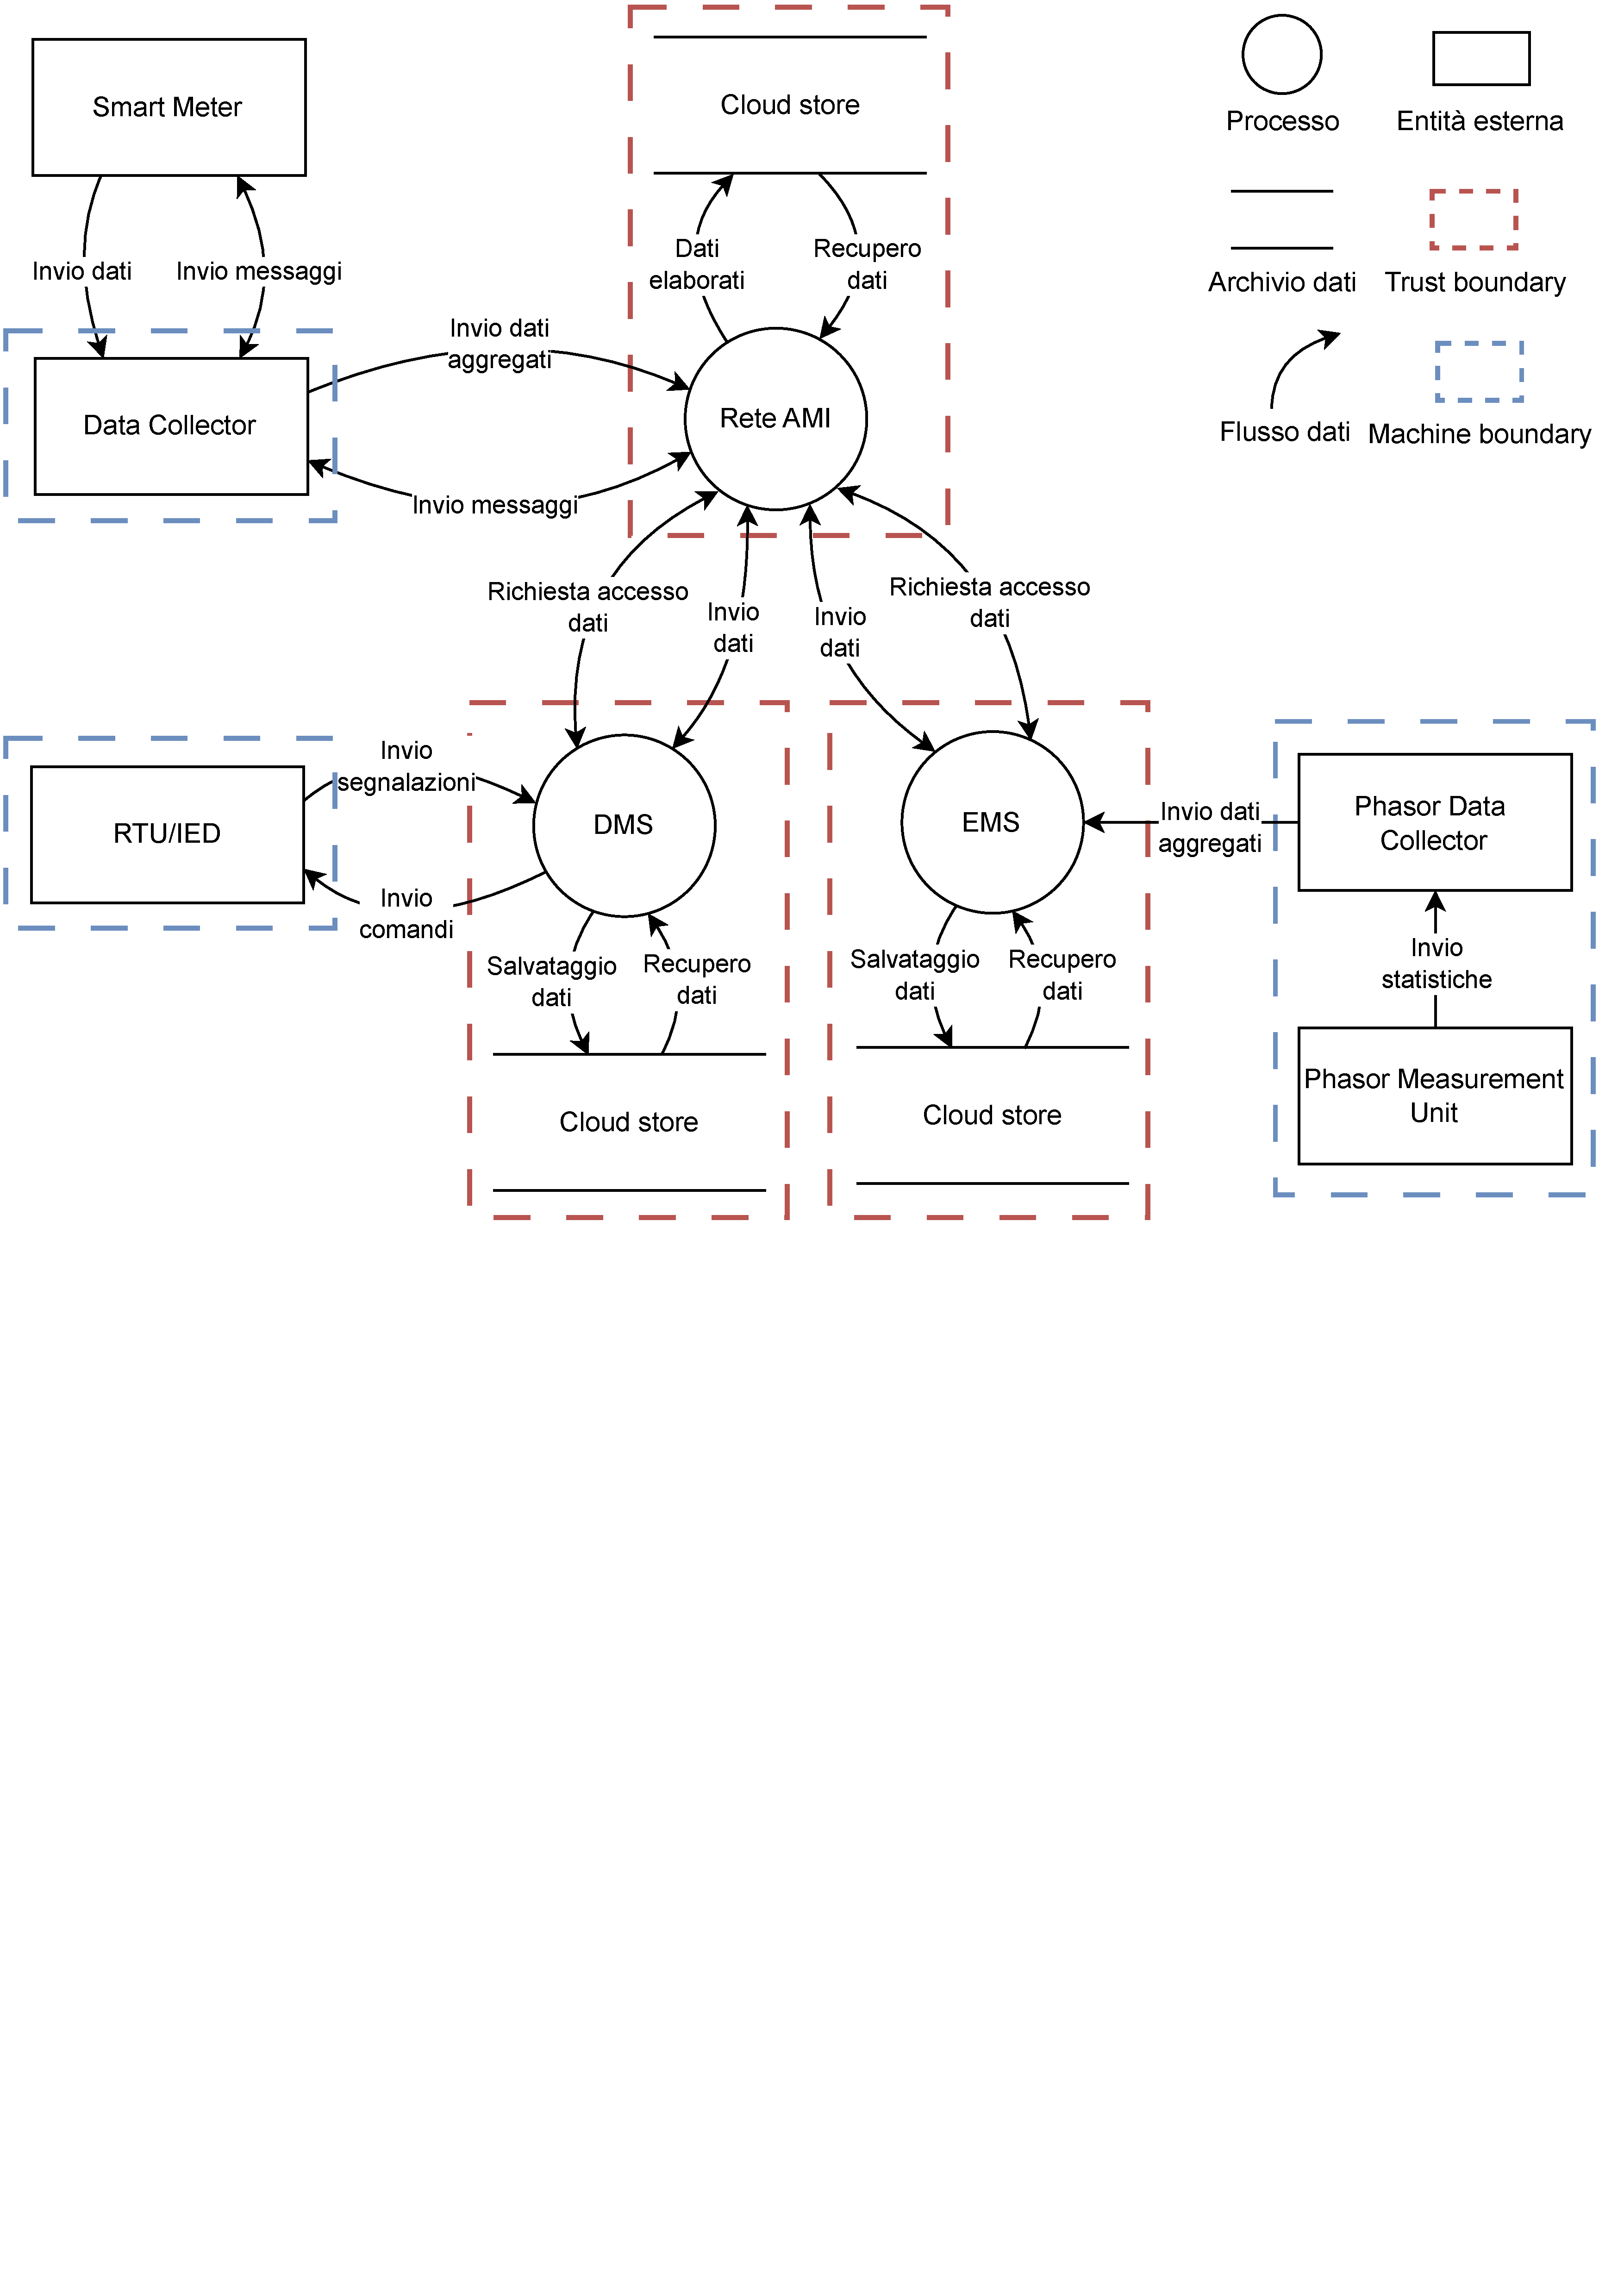
\includegraphics[trim= 0cm 39cm 0cm 0cm, clip, width=0.8\linewidth]{img/DFD.drawio.pdf}
%     \caption{Data flow diagram - Smart Grid Cloud-Native}
%     \label{fig:DFD}
% \end{figure}


% \subsection{Definizione dell'Ambito di Analisi}

% % Nella Tabella \ref{tab:def-ambito} troviamo la definizione degli elementi: \textit{In scope}, ovvero all'interno dell'ambito di ricerca di questa tesi; \textit{Out od scope}, che non fanno parte prettamente all'infrastruttura cloud della Smart Grid. 

% Prima di procedere con l'analisi delle minacce, è essenziale definire con precisione il perimetro (o scope) di questo studio. Data la vastità dell'ecosistema Smart Grid, l'analisi si concentrerà specificamente sulle vulnerabilità introdotte dalla sua implementazione in un'architettura Cloud-Native.


% Di conseguenza, verranno prese in considerazione le minacce relative ai componenti software centralizzati e ai canali di comunicazione che li collegano al campo. 
% % Le problematiche di sicurezza legate strettamente all'hardware dei dispositivi Edge – come la manomissione fisica, gli attacchi a livello di firmware o le vulnerabilità dei circuiti integrati – pur essendo di fondamentale importanza per la sicurezza complessiva, sono considerate al di fuori dell'ambito di questa tesi per mantenere un focus mirato sulle minacce a livello di architettura di rete e applicativa.


% La Tabella \ref{tab:def-ambito} riassume formalmente questa suddivisione, elencando gli elementi considerati oggetto di analisi (\textit{In Scope}) e esclusi dall'analisi (\textit{Out of Scope}).

% % \begin{table}[h!]
% %     \centering
% %     % \renewcommand{\arraystretch}{1.5}
    
% %     \begin{tabular}{c|c|c}
% %          &  \textbf{In scope} & \textbf{Out of scope}\\
% %          \hline
% %          &  & \\
% %          Componenti  &   HES, MDMS, DMS, EMS, & Sicurezza dei dispositivi hardware: SM, DC, \\         
% %          software: &   SCADA, GMS, High-level PDC & RTU/IED, Generatori, low-level PDC, PMU\\
% %         &  & \\
         
% %          Canali di &  PLC/RF $169\,MHz$, 4G/5G,&  Sicurezza della cabina Telco\\
% %          comunicaizone: &    Fibra, VPN  & \\
% %           &  & \\
% %          Infrastruttura cloud:&  Kubernetes e container & \\
% %           &  & \\
% %     \end{tabular}
% %     \caption{Definizione dell'ambito}
% %     \label{tab:def-ambito}
% % \end{table}

% \renewcommand{\arraystretch}{1.5}
% \begin{longtable}[!h]{p{5cm}p{5cm}p{5cm}}
        
%     \caption{Definizione dell'ambito di analisi} 
%     \label{tab:def-ambito}\\
    
%     \hline
%     &  \textbf{Oggetto in analisi} & \textbf{Oggetto fuori dall'analisi}\\
%     \hline
%     \endfirsthead
    
%     \hline
%     &  \textbf{Oggetto in analisi} & \textbf{Oggetto fuori dall'analisi}\\
%     \hline
%     \endhead

%     Componenti software: &   SM, HES, MDMS, DMS, EMS, SCADA, GMS, High-level PDC & Sicurezza dei dispositivi hardware: DC, RTU/IED, Generatori, low-level PDC, PMU\\
    
%     Canali di comunicaizone: &  PLC/RF $169\,MHz$, 4G/5G, Fibra, VPN&  Sicurezza della cabina Telco\\
         
%     Infrastruttura cloud:&  Kubernetes e container & \\

    
%     \hline
% \end{longtable}


% \subsection{Identificazione degli Asset Critici}

% % Nella seguente Tabella \ref{tab:def-asset}, in ogni colonna, sono presentati una serie di asset


% % \begin{table}[h!]
% %     \centering
% %     \renewcommand{\arraystretch}{1.5}
    
% %     \begin{tabular}{c|c|c}
% %          \textbf{Dati} &  \textbf{Processi} & \textbf{Infrastruttura logica}\\
% %          \hline
% %          Statistiche del cliente   &    dati collezionati da HES & Cluster K8s  \\         
% %          Fatturazione consumi (MDMS) &   elaborazione dei dati MDMS & Immagini container \\
% %          Statistiche di rete (PMU) &  monitoraggio della rete EMS/DMS & Infrastruttura VPN \\
         
% %          API, credenziali, token & Dati collezionati da high-level PDC & Cloud storage  \\

% %     \end{tabular}
% %     \caption{Definizione degli asset}
% %     \label{tab:def-asset}
% % \end{table}



% Successivamente alla definizione della struttura del sistema tramite il DFD, è cruciale identificare gli asset, ovvero gli elementi di valore all'interno dell'architettura la cui compromissione causerebbe un danno significativo. Sapere cosa si sta proteggendo è un prerequisito fondamentale per poter valutare l'impatto reale di una minaccia.
% Un'analisi completa considera che gli asset non sono limitati ai soli dati, ma includono anche i processi e i componenti infrastrutturali che li gestiscono. Per questa tesi, gli asset sono stati classificati in tre tipologie principali:

% \begin{enumerate}
%     \item \textbf{Dati:} Rappresentano le informazioni sensibili o critiche gestite dal sistema. La loro compromissione può portare a violazioni della privacy, frodi o perdita di controllo sulla rete. Esempi includono i dati di consumo dei clienti, le statistiche di rete delle PMU e le credenziali di accesso come token e chiavi API.
%     \item \textbf{Processi:} Sono le funzioni operative e di elaborazione chiave del sistema. Un attacco a un processo può corrompere i dati, causare un'interruzione del servizio o portare a decisioni errate nella gestione della rete. Esempi includono l'elaborazione dei dati da parte dell'MDMS o il monitoraggio della rete da parte dell'EMS.
%     \item \textbf{Infrastruttura Logica:} Costituisce la base tecnologica su cui poggia l'intera architettura. La compromissione di questi componenti può avere un impatto a cascata su tutti i servizi ospitati. Esempi includono i cluster Kubernetes, le immagini dei container e l'infrastruttura VPN che garantisce la comunicazione sicura.
% \end{enumerate}

% La Tabella \ref{tab:def-asset} presenta una sintesi dei principali asset identificati per l'architettura in esame, classificati secondo queste tre tipologie.

% \renewcommand{\arraystretch}{1.5}
% \begin{longtable}[!h]{p{5cm}p{5cm}p{5cm}}
        
%     \caption{Identificazione degli Asset Critici}
%     \label{tab:def-asset}\\
    
%     \hline
%     \textbf{Dati} &  \textbf{Processi} & \textbf{Infrastruttura logica}\\
%     \hline
%     \endfirsthead
    
%     \hline
%     \textbf{Dati} &  \textbf{Processi} & \textbf{Infrastruttura logica}\\
%     \hline
%     \endhead
    
    
%     Statistiche del cliente   &    dati collezionati da HES & Cluster K8s  \\         
%     Fatturazione consumi (MDMS) &   elaborazione dei dati MDMS & Immagini container \\
%     Statistiche di rete (PMU) &  monitoraggio della rete EMS/DMS & Infrastruttura VPN \\    
%     API, credenziali, token & Dati collezionati da high-level PDC & Cloud storage  \\
    
    
%     \hline
% \end{longtable}


% \section{Analisi delle Minacce con il Framework STRIDE}

% Dopo aver modellato il sistema, si procede ora con la fase di identificazione delle minacce, il cuore di questa analisi. Come anticipato, questa fase verrà condotta applicando sistematicamente il framework STRIDE e utilizzando come riferimento il Data Flow Diagram Figura \ref{fig:DFD}.


% L'approccio utilizzato sarà quello di \textbf{STRIDE-per-elemento}: per ogni componente del DFD (processi, data store, flussi di dati ed entità esterne), verranno considerate le categorie di minaccia STRIDE pertinenti. Questo metodo garantisce una copertura completa e strutturata, riducendo il rischio di tralasciare vulnerabilità significative.




% % \renewcommand{\arraystretch}{1.5}
% % \begin{longtable}{p{1.5cm}p{2cm}p{2cm}p{6.5cm}p{3cm}}
% %     \caption{Minacce informatiche}
% %     \label{tab:minacce-info} \\
    
% %     \hline
% %     \textbf{ID Minaccia} &\textbf{Elemento} & \textbf{Categoria STRIDE}& \textbf{Descrizione minaccia} & \textbf{Possibile attaccante} \\
% %     \hline
% %     \endfirsthead
    
% %     \hline
% %     \textbf{ID Minaccia} &\textbf{Elemento} & \textbf{Categoria STRIDE} & \textbf{Descrizione minaccia} &\textbf{Possibile attaccante} \\
% %     \hline
% %     \endhead

% %     S-01 & Cluster K8s & \textbf{S}poofing, Elevation of Privilege & Service Account Impersonation: un attaccante sfrutta una vulnerabilità di un pod per impossessarsi della private key del suo Service Account e lo usa per accedere alle API di K8s, impersonando il servizio per leggere configurazione e lanciare altri pod malevoli. & Attaccante esterno che ha ottenuto un accesso iniziale; insider\\
    
% %     T-01 & Nodi worker K8s &  \textbf{T}ampering, Elevation of Privilege & Un attaccante sfruttando una vulnerabilità del cloud provider, modifica in una qualsiasi parte il worker node di K8s permettendogli di inserire del codice malevole per prenderne il possesso. & Attaccante molto competente\\

% %     T-02 & Comunicazioni & \textbf{T}ampering & Un attaccante riesce ad intercettare la comunicazione, da e/o verso un servizio cloud, modificandone i dati di consumo o comandi di esecuzione. Man-in-the-middle attack. & Attaccante esterno con accesso alla rete di comunicazione (PLC, VPN, Fibra)\\

% %     R-01 & Invio comandi & \textbf{R}epudiation & Un operatore di un sistema (EMS/DMS) invia un comando alla rete, di trasformazione, produzione, ecc., legittimo ma dannoso per errore e poi nega di averlo fatto. La mancanza di log immutabili e firmati digitalmente rende impossibile l'attribuzione del fatto. & Operatore interno \\
    

% %     I-01 & Flussi dati & \textbf{I}nformation Disclosure & A causa di regole di firewall assenti o troppo permissive tra i cluster K8s, un attaccante può sfruttare le porte lasciate aperte per sferrare l'attacco & Attaccante esterno \\

% %     I-02 & Comunicazione in entrata & \textbf{I}nformation Disclosure & Le regole impostate del firewall risultano essere troppo permissive, esponendo su internet i nodi dei cluster, incluse porte sensibili come la porta 22 (SSH) la quale può essere presa di mira dagli attaccanti. & Attaccante esterno \\

% %     I-03 & Dati salvati & \textbf{I}nformation Disclosure & Un utente interno o un possibile attaccante sfruttando configurazioni errate del cloud storage per accedere ai dati dei clienti o allo stato della rete. & Insider; Attaccante esterno\\

% %     D-01 & Disponibilità servizio & \textbf{D}enial of Service & Un attaccante lancia un attacco DDoS contro gli endpoint della della rete, impedendo agli operatori l'analisi della rete in tempo reale & Attaccante esterno \\

% %     E-01 & Cluster K8s & \textbf{E}levation of Privilege &  Non rispetto del principio del minimo privilegio, assegnando al personale ruoli di accesso non pertinenti alla sua mansione & Insider\\

% %     E-02 & \textbf{E}levation of Privilege & Processi interni al cluster K8s & Un attaccante, dopo aver compremesso un pod con bassi privilegi, sfrutta una vulnerabilità del container runtime o del kernel per ottenere l'accesso root sul nodo, potendo così inviare messaggi malevoli alla rete & Attaccante esterno \\
   

% % \hline

% % \end{longtable}


% \renewcommand{\arraystretch}{1.5}
% \begin{longtable}{p{1.5cm}p{2cm}p{2cm}p{7.5cm}p{2cm}}
%     \caption{Minacce informatiche}
%     \label{tab:minacce-info} \\
    
%     \hline
%     \textbf{ID Minaccia} &\textbf{Elemento} & \textbf{Categoria STRIDE}& \textbf{Descrizione minaccia} & \textbf{Possibile attaccante} \\
%     \hline
%     \endfirsthead
    
%     \hline
%     \textbf{ID Minaccia} &\textbf{Elemento} & \textbf{Categoria STRIDE} & \textbf{Descrizione minaccia} &\textbf{Possibile attaccante} \\
%     \hline
%     \endhead

%     S-01 & Smart Meter & \textbf{S}poofing & Una mancanza di risorse e memoria limitata su SM e dispositivi di campo, possono impedire l'implementazione di tutte le funzionalità di sicurezza e l'aggiornamento del firmware, rendendoli più vulnerabili ad attaccanti esperti che riescono a sfruttare queste vulnerabilità minando l'affidabilità dei dati inviati ai DC. \cite{paper-threat-modelling}& Attaccante esterno\\
    
%     T-01 & Flusso dati PDC & \textbf{T}ampering & Un attaccante non si limita ad un possibile DoS bloccando i dati inviati dai PDC su rete 4G/5G, bensì cerca di intercettare il traffico e modificare leggermente e costantemente tutti i dati prima che essi raggiungano l'EMS. Questo attacco simula un \textbf{carico fantasma} o una falsa instabilità di frequenza. L'EMS che si fida di questi dati reagisce automaticamente ridirigendo l'energia o sezionando la zona, causando gravi disagi. \cite{paper-threat-modelling}& Attaccante esterno\\

%     R-01 & Dati consumatori & \textbf{R}epudiation & Un attaccante esterno, riuscendo ad avere accesso privilegiato con permessi di lettura e scrittura al cloud store dell'infrastruttura AMI, riesce a modificare i dati contenuti nel database con conseguente impatto sulle misure fino ad ora effettuate e possibili previsioni future. & Attaccante esterno \\
    

%     I-01 & Software di gestione & \textbf{I}nformation Disclosure & Un attaccante può sfruttare le vulnerabilità scoperte nei software open source, come ad esempio OpenEMS, per compromettere i sistemi EMS delle aziende che li utilizzano. Alternativamente, l'attaccante può inserire codice malevolo nel progetto open source, che successivamente utilizzerà per condurre attacchi mirati all'esfiltrazione dei dati dell'azienda. & Attaccante esterno\\

%     D-01 & Disponibilità servizio & \textbf{D}enial of Service & L'attaccante riesce ad accedere alle cabine secondarie del DSO e si collega tramite uno switch tra il gateway e la RTU. Questa posizione privilegiata gli consente di intercettare il traffico di rete e identificare il server SCADA presente nel DMS. Una volta individuato il target, l'attaccante può lanciare un attacco DoS (magari utilizzando di un software come \textit{hping}) contro il servizio cloud che ospita il cluster Kubernetes, saturando il canale di trasmissione e causando latenze significative (\textit{Bottleneck}). Queste latenze compromettono gravemente l'invio tempestivo dei dati di telemetria, delle segnalazioni e dei comandi di controllo provenienti dallo SCADA Master, causando potenziali disfunzioni operative nella rete di distribuzione. \cite{threat-sotto-stazioni-paper} & Attaccante esterno\\ 
    

%     E-01 & Invio comandi & \textbf{E}levation of Privilege & Una volta ottenuto il controllo di un cluster Kubernetes del DMS sfruttando l'endpoint API utilizzato per l'invio delle segnalazioni da parte di RTU/IED, un attaccante può evitare di causare un singolo e vistoso disservizio, optando invece per sfruttare le capacità del DMS di controllare migliaia di dispositivi sul campo (RTU/IED) per lanciare un attacco distribuito e coordinato. L'attaccante può inviare comandi di apertura e chiusura degli interruttori o regolare la tensione dei trasformatori, causando oscillazioni di frequenza e tensione su tutta la rete di distribuzione, con effetti che possono propagarsi fino a perturbare la rete di alta tensione. & Attaccante esterno con aiuto da insider\\
   

% \hline


% \end{longtable}




% \section{Strategie di Mitigazione e Contromisure di Sicurezza}


% \renewcommand{\arraystretch}{1.5}
% \begin{longtable}{p{1.5cm}p{3.5cm}p{8cm}p{2.5cm}}
    
    
%     \caption{Mitigazione delle minacce} \\
    
%     \hline
%     \textbf{ID Minaccia }& \textbf{Descrizione minaccia} & \textbf{Mitigazione proposta} & \textbf{Categoria mitigazione}\\
%     \hline
%     \endfirsthead
    
%     \hline
%     \textbf{ID Minaccia }& \textbf{Descrizione minaccia} & \textbf{Mitigazione proposta} & \textbf{Categoria mitigazione}\\
%     \hline
%     \endhead

%     S-01 & Impersonificazione di SM & Durante la fase di acquisto dei dispositivi da utilizzare per centinaia di migliaia di dispositivi, il DSO deve imporre requisiti di sicurezza minimi obbligatori durante il bando di gare. L'utilizzo di pattern statistici e algoritmi di \textit{Anomaly Detection} da parte dell'AMI, può essere d'aiuto per valutare eventuali dispositivi compromessi. & Mitigare \\
    
%     T-01 & Manomissione dati in transito & L'utilizzo di crittografia e autenticazione End-to-End può rendere la manomissione dei dati difficile. L'EMS non si dovrebbe fidare ciecamente bensì deve tutelarsi incrociando dati da altri dispositivi utilizzando pattern statistici di correlazione. \cite{paper-threat-modelling} & Mitigazione \\

%     R-01 & Furto e/o modifica dei dati AMI & I dati una volta validati devono essere archiviati in un database \textit{WORM} (Write-Once, Read-Many) garantendo la non mutabilità del dato. Nessuna singola persona, a presciendere dal ruolo, dovrebbe avere i permessi per leggere, modificare e cancellare dati sensibili, sia di utenti sia aziendali. & Mitigazione.\\

%     I-01 & Inserimento di codice malevolo & Verificare attraverso code review l'utilizzo delle \textit{Best Practices} di sicurezza, implementative e le ulteriori librerie open-sorce utilizzate & Accettarlo \\

%     D-01 & Minare il funzionamento dello SCADA Master & La simulazione ha rivelato che il collo di bottiglia delle prestazioni durante un attacco DoS erano i router, la cui CPU veniva utilizzata al $100\%$, rendendoli irresponsabili sia tramite interfaccia web che CLI. Al contrario, il dispositivo di monitoraggio (che simula il server SCADA) ha mostrato un impatto minimo sull'utilizzo di CPU e RAM. Questo suggerisce che se il router è il punto debole, una parte significativa del traffico d'attacco può essere bloccata a quel livello, impedendo che raggiunga il server SCADA e potenzialmente l'intera rete attraverso l'impostazione di regole firewall appropriate \cite{threat-sotto-stazioni-paper}  &  Mitigarlo \\

%     E-01 & Attacco distribuito MT/BT & Nessun singolo processo deve avere la possibilità di controllare tutti i dispositivi di campo. I privilegi di comando devono essere segmentati geograficamente e/o per dispositivo, seguendo il modello RBAC. Inoltre per comandi ad alto impatto deve essere predisposto almeno una seconda approvazione da parte del personale. & Mitigazione\\
%     \hline
% \end{longtable}


% % PAPER DoS

% % Le fonti indicano che la mitigazione principale proposta per gli attacchi Denial of Service (DoS) è l'implementazione di configurazioni appropriate dei firewall.
% % Questa raccomandazione deriva direttamente dalle scoperte dello studio, che ha classificato gli attacchi DoS come i più critici tra le categorie di minacce identificate dal modello STRIDE. Ecco perché l'uso dei firewall è considerato cruciale:
% % •
% % Elevata criticità degli attacchi DoS: Gli attacchi DoS sono stati identificati come la categoria più critica di minacce, avendo il maggior numero di minacce ad alta priorità che necessitano di indagine (8 su 24 totali). La loro elevata probabilità di accadimento è dovuta alla possibilità di essere eseguiti con un singolo comando utilizzando strumenti disponibili pubblicamente come hping3, che non richiedono conoscenze specialistiche.
% % •
% % Impatto sulla comunicazione e sul controllo: La simulazione ha dimostrato che un traffico d'attacco di circa 14 Mbps con circa 30.000 pacchetti al secondo (PPS) è sufficiente a interrompere la comunicazione IEC104. Un attacco DoS riuscito può portare alla perdita dell'osservabilità e della controllabilità dell'intera smart grid.
% % •
% % Identificazione del "collo di bottiglia": I test nel modello di simulazione hanno rivelato che il collo di bottiglia delle prestazioni durante un attacco DoS erano i router, la cui CPU veniva utilizzata al 100%, rendendoli irresponsabili sia tramite interfaccia web che CLI. Questo è significativo perché, al contrario, il dispositivo di monitoraggio (che simulava il server SCADA) ha mostrato un impatto minimo sull'utilizzo di CPU e RAM.
% % •
% % Strategia di mitigazione: Poiché i router sono il punto debole in questo scenario, bloccare il traffico d'attacco a questo livello, ad esempio tramite firewall opportunamente configurati sui router stessi o a monte di essi, impedirebbe che la maggior parte del traffico dannoso raggiunga il server SCADA e potenzialmente l'intera rete. Se l'attacco riuscisse a bypassare le difese a livello di router e a raggiungere direttamente il server SCADA, avrebbe un potenziale maggiore di esaurire le risorse del server, causando la completa perdita di osservabilità e controllabilità dell'intera rete.
% % •
% % Applicazione pratica: Le aziende della rete elettrica in Norvegia stanno già utilizzando i risultati di questo studio per migliorare le proprie misure di sicurezza, specialmente contro gli attacchi DoS, proprio attraverso l'adozione di appropriate configurazioni dei firewall.
% % In sintesi, la mitigazione tramite configurazioni dei firewall si concentra sulla protezione dei punti di ingresso e degli elementi di rete critici (come i router) che fungono da "collo di bottiglia" per il traffico, prevenendo così che attacchi DoS facilmente eseguibili compromettano la funzionalità dell'intera smart grid.


% % \renewcommand{\arraystretch}{1.5}
% % \begin{longtable}{p{1.5cm}p{3.5cm}p{8cm}p{2.5cm}}
    
    
% %     \caption{Mitigazione delle minacce} \\
    
% %     \hline
% %     \textbf{ID Minaccia }& \textbf{Descrizione minaccia} & \textbf{Mitigazione proposta} & \textbf{Categoria mitigazione}\\
% %     \hline
% %     \endfirsthead
    
% %     \hline
% %     \textbf{ID Minaccia }& \textbf{Descrizione minaccia} & \textbf{Mitigazione proposta} & \textbf{Categoria mitigazione}\\
% %     \hline
% %     \endhead
    
% %     S-01 &  Service Account Impersonation& Principio di minimo privilegio: creare ruoli RBAC specifici e restrittivi per ogni Service Account evitando di inserire tutti i privilegi. Gestire le credenziali in modo opportuno utilizzando nei \textit{Secrets}, oggetti contenenti questi dati molto sensibili  & Mitigarla \\


% %     T-01 &  Attacco sfruttando vulnerabilità cloud provider & Google Cloud offre la possibilità di abilitare la funzionalità "Shielded Nodes". Garantisce un \textbf{avvio sicuro} dato che guarda se il software sia firmato digitalmente e non manomesso. Crea una hash dello stato di avvio e monitora che non cambi nel tempo.  & Mitigarla\\

% %     T-02 & Manomissione dati in transito & Utilizzo di cifratura asimmetrica sul canale di comunicazione (TLS) e codici di autenticazione e firma del messaggio per garantirne l'integrità (integrity). & Mitigarla \\

% %     R-01 & Ripudio di un comando inviato & Tutti i comandi, critici e non, devono essere firmati digitalmente dall'operatore e finire nel Audit Log per mantenerne traccia di tutte le operazioni rendendole sicure ed immutabili. Possono essere usati ledger blockchain o servizi che permettono solo log write-once & Eliminarla\\
    
    
% %     I-01 &  Regole firewall non adatte & Definire una solida regola di Network Policies in K8s per definire quali pod possono comunicare con quali altri pod, su quale IP, porta e protocollo magari definendo regole di \textit{Ingress} e \textit{Egress} & Mitigarla\\

% %     I-02 &  Configurazione errata firewall & L'utilizzo della rete Virtual Private Cloud (VPC) permette di sopperire ad un'errata configurazione del firewall  rendendo la comunicazioni privata tra i soli componenti della rete VPC. Eliminazione degli IP pubblici quando questi non sono strettamente necessari e accesso tramite rete VPN. & Mitigarla\\

% %     I-03 & Configurazione errata cloud storage & Applicazione di algoritmi per cifrare i dati presenti nel cloud store. Utilizzare policy di identificazione e ruolo con il principio del minimo privilegio. & Mitigarla\\

% %     D-01 & DDoS contro endpoint critici & Utilizzare servizi di anti-DDoS a livello di rete. Implementare il \textit{rate limiting} sugli endpoint API dei cluster K8s. Avere un piano nel caso questo evento dovesse comunque succedere. & Mitigare, Accettarla\\

% %     E-01 &  Non rispetto del Principio di minimo privilegio & Cercare di fare attenzione quando si inseriscono i privilegi ad un utente  & Mitigarla\\

% %     E-02 & Elevation of Privilege nel cluster K8s & Eseguire i container come utenti non-root ed utilizzare policy di sicurezza a livello di pod & Mitigarla \\
    
% %     \hline
% % \end{longtable}


% \section{Approcci alla Validazione delle Contromisure}

% La fase finale del ciclo di Threat Modeling, la validazione, è essenziale per garantire che le contromisure proposte siano efficaci e che la postura di sicurezza complessiva del sistema sia stata effettivamente migliorata. Sebbene un'implementazione e una validazione empirica completa dell'architettura proposta esulino dall'ambito di questa tesi, è possibile delineare un piano di validazione strutturato.

% Questo piano si baserebbe su una combinazione di revisioni di progettazione e test di sicurezza pratici, mirati a verificare le mitigazioni suggerite.

% \begin{enumerate}
%     \item \textbf{Revisione e Analisi del Rischio Residuo:}
%     \\Il primo passo consisterebbe in una revisione formale delle contromisure progettate per ogni minaccia. Per ciascuna, si dovrebbe valutare il rischio residuo, ovvero il livello di rischio che permane anche dopo l'implementazione della mitigazione. L'obiettivo è assicurarsi che tale rischio sia sceso al di sotto della soglia di accettabilità definita dagli stakeholder del sistema.
%     \item \textbf{Test di Sicurezza a Livello di Infrastruttura Cloud-Native:}
%     \\Per validare le contromisure legate alla configurazione di Kubernetes e dei container, si potrebbero eseguire le seguenti attività:
%     \begin{itemize}
%         \item Scansione delle Immagini dei Container: Utilizzare strumenti come Trivy o Clair per scansionare le immagini dei container (HES, DMS, etc.) alla ricerca di vulnerabilità note in librerie e dipendenze.
%         \item Analisi della Configurazione del Cluster (IaC Scanning): Impiegare strumenti come Kube-bench o Checkov per analizzare i file di configurazione di Kubernetes (Infrastructure as Code) e verificare che siano conformi alle best practice di sicurezza del CIS (Center for Internet Security).
%     \end{itemize}
%     \item \textbf{Test di Sicurezza a Livello Applicativo e di Rete:}
%     \\Per verificare le contromisure a livello di servizio, si potrebbero pianificare test più attivi:
%     \begin{itemize}
%         \item Penetration Testing mirato: Eseguire test di penetrazione focalizzati sui punti più critici emersi dall'analisi STRIDE. Ad esempio, si potrebbe tentare di sfruttare una debolezza nelle API esposte dal cluster EMS o di effettuare un attacco di Tampering sui dati scambiati tramite la VPN inter-cluster.
%         \item Creazione di Security Test Case: Sviluppare test automatici che verifichino specifiche contromisure. Ad esempio, un test potrebbe simulare una richiesta con un token di autenticazione invalido per assicurarsi che venga correttamente respinta, validando così una mitigazione contro lo Spoofing.
%     \end{itemize}
% \end{enumerate}


% L'esecuzione di queste attività di validazione fornirebbe un feedback concreto sull'efficacia delle strategie di mitigazione proposte e completerebbe il ciclo iterativo del Threat Modeling, trasformando l'analisi teorica in una base solida per un'implementazione sicura.

      \newpage
\chapter{Conclusioni}
      

\begin{figure}[!ht]
    \centering
    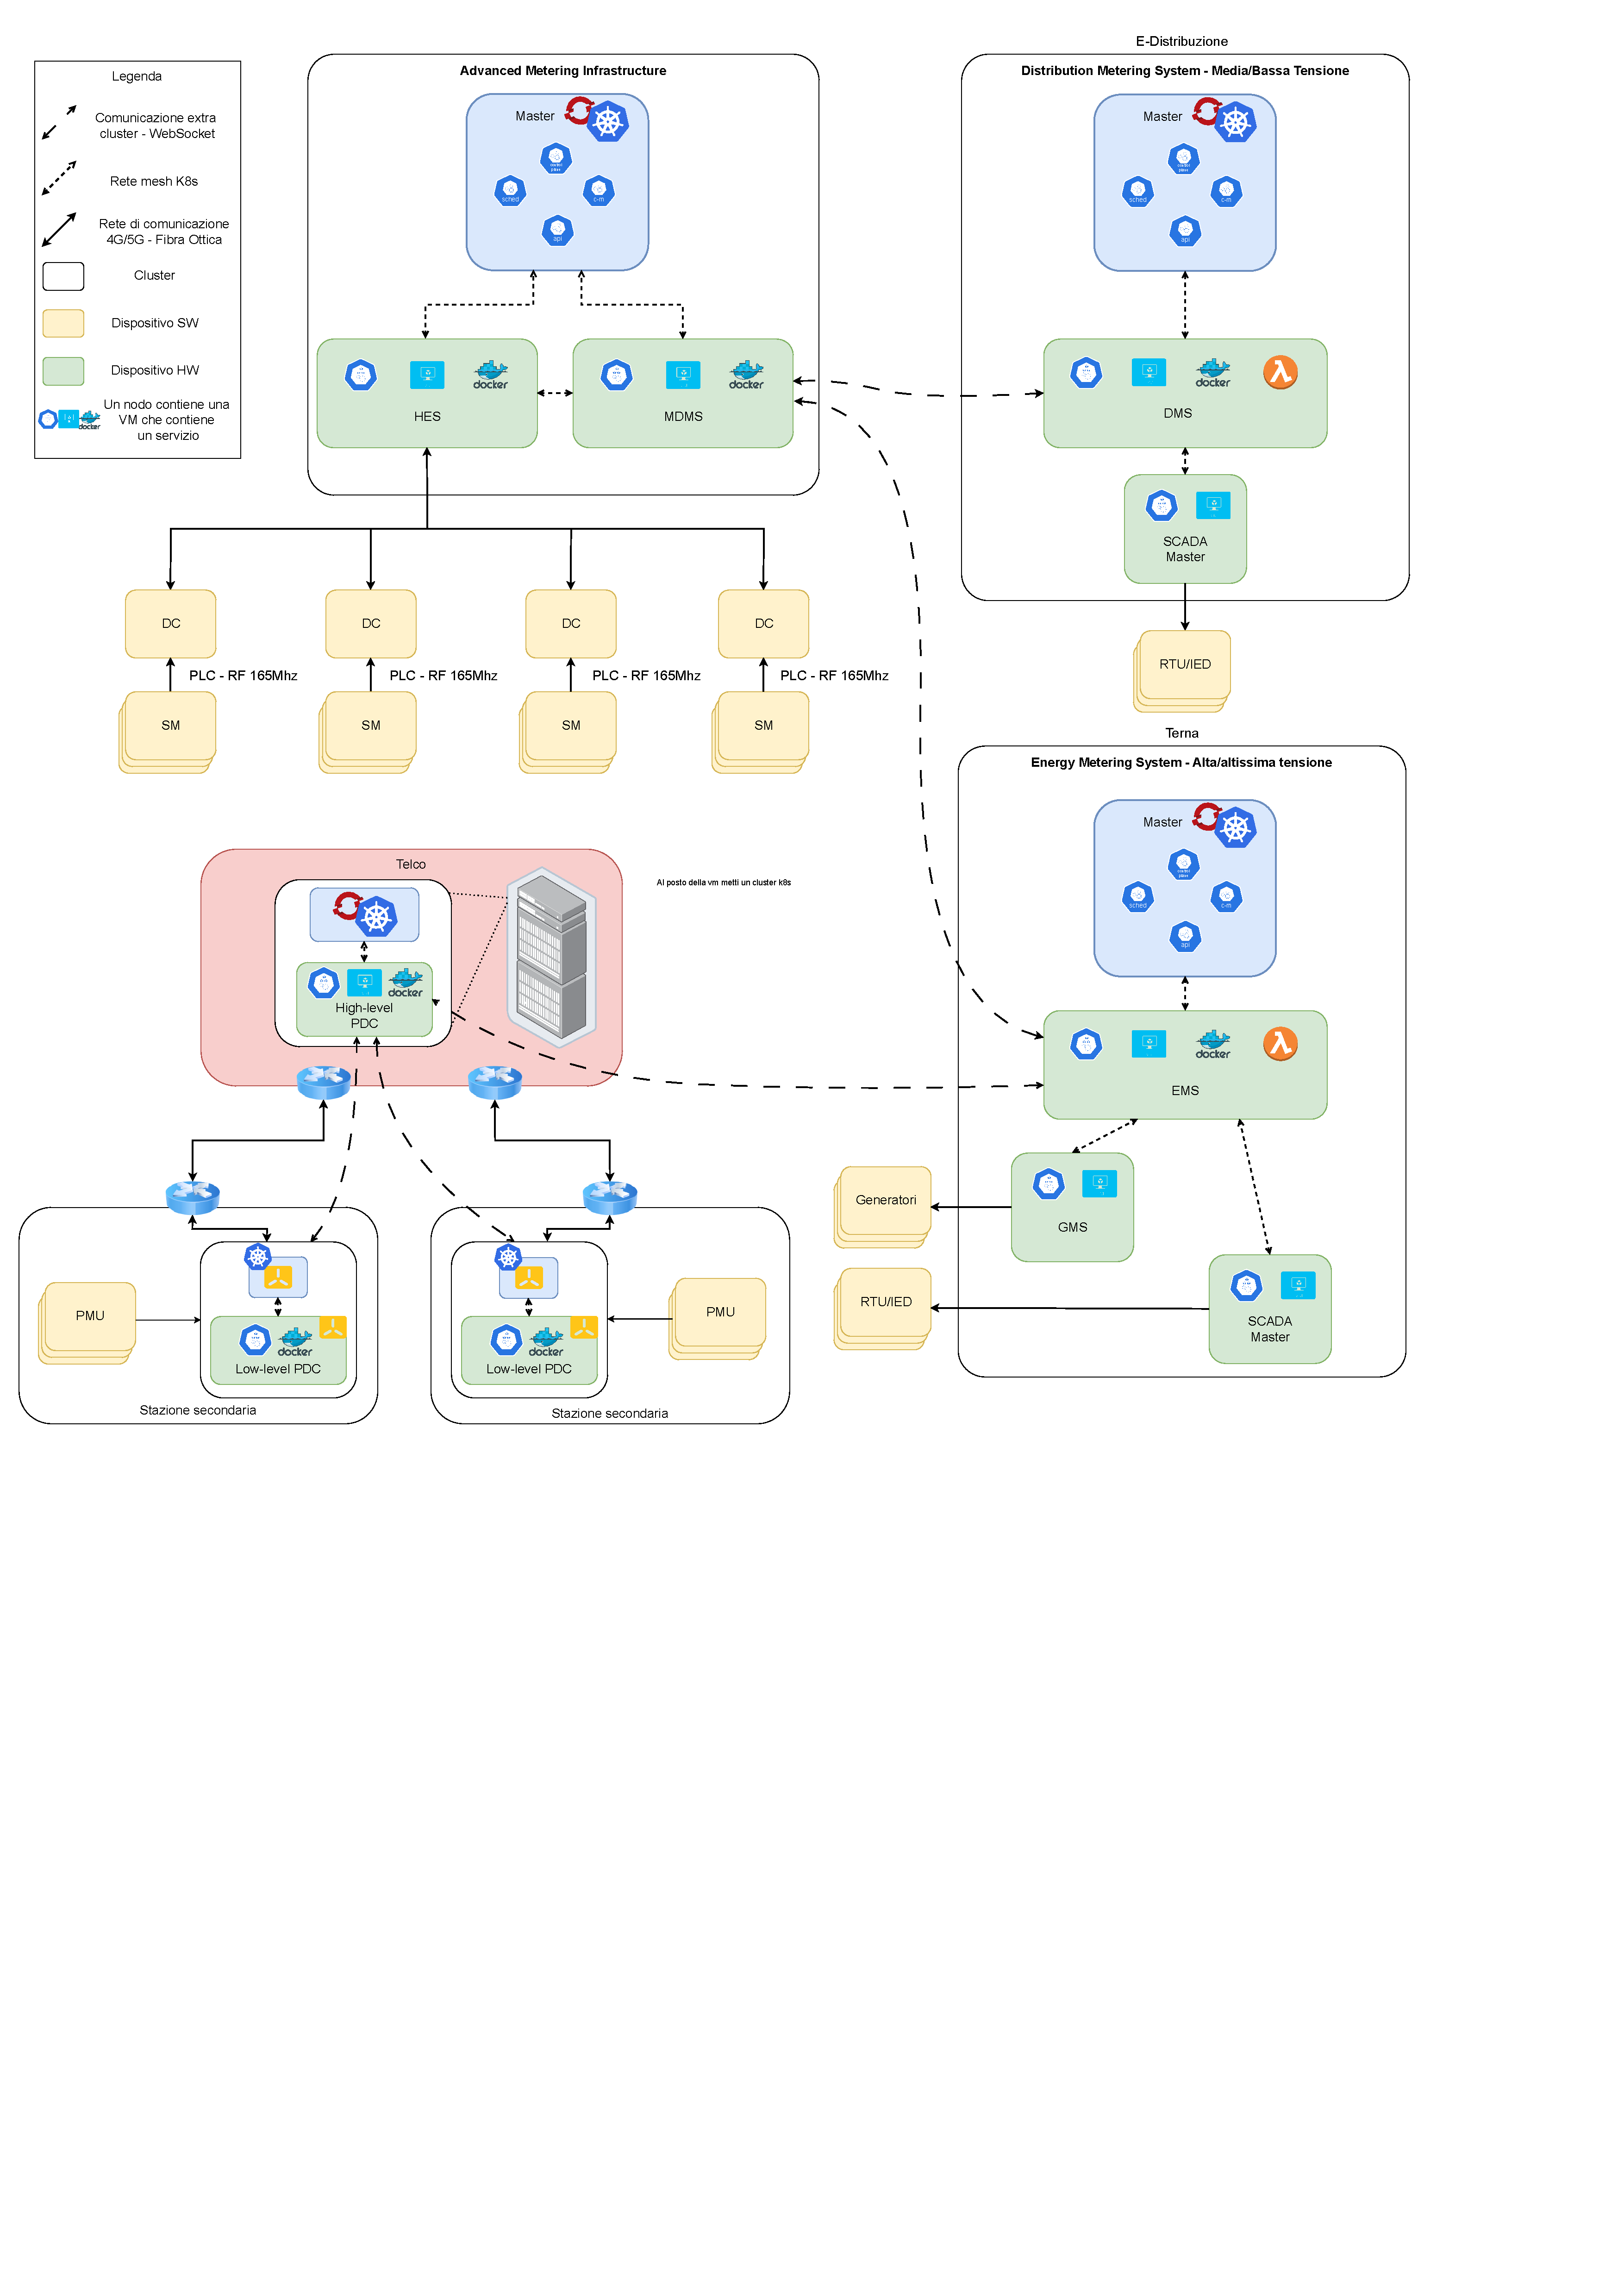
\includegraphics[trim= 0cm 31cm 7.8cm 0cm, clip, width=0.97\linewidth]{img/aa.pdf}
    \caption{Class Diagram}
\end{figure}
      
      
    \endgroup


    % bibliografia in formato bibtex
    %
    % aggiunta del capitolo nell'indice
    \addcontentsline{toc}{chapter}{Bibliografia}
    % stile con ordinamento alfabetico in funzione degli autori
    \bibliographystyle{plain}
    \bibliography{biblio}
%%%%%%%%%%%%%%%%%%%%%%%%%%%%%%%%%%%%%%%%%%%%%%%%%%%%%%%%%%%%%%%%%%%%%%%%%%
%%%%%%%%%%%%%%%%%%%%%%%%%%%%%%%%%%%%%%%%%%%%%%%%%%%%%%%%%%%%%%%%%%%%%%%%%%
%% Nota
%%%%%%%%%%%%%%%%%%%%%%%%%%%%%%%%%%%%%%%%%%%%%%%%%%%%%%%%%%%%%%%%%%%%%%%%%%
%% Nella bibliografia devono essere riportati tutte le fonti consultate 
%% per lo svolgimento della tesi. La bibliografia deve essere redatta 
%% in ordine alfabetico sul cognome del primo autore. 
%% 
%% La forma della citazione bibliografica va inserita secondo la fonte utilizzata:
%% 
%% LIBRI
%% Cognome e iniziale del nome autore/autori, la data di edizione, titolo, casa editrice, eventuale numero dell’edizione. 
%% 
%% ARTICOLI DI RIVISTA
%% Cognome e iniziale del nome autore/autori, titolo articolo, titolo rivista, volume, numero, numero di pagine.
%% 
%% ARTICOLI DI CONFERENZA
%% Cognome e iniziale del nome autore/autori (anno), titolo articolo, titolo conferenza, luogo della conferenza (città e paese), date della conferenza, numero di pagine. 
%% 
%% SITOGRAFIA
%% La sitografia contiene un elenco di indirizzi Web consultati e disposti in ordine alfabetico. 
%% E’ necessario:
%%   Copiare la URL (l’indirizzo web) specifica della pagina consultata
%%   Se disponibile, indicare il cognome e nome dell’autore, il titolo ed eventuale sottotitolo del testo
%%   Se disponibile, inserire la data di ultima consultazione della risorsa (gg/mm/aaaa).    
%%%%%%%%%%%%%%%%%%%%%%%%%%%%%%%%%%%%%%%%%%%%%%%%%%%%%%%%%%%%%%%%%%%%%%%%%%
%%%%%%%%%%%%%%%%%%%%%%%%%%%%%%%%%%%%%%%%%%%%%%%%%%%%%%%%%%%%%%%%%%%%%%%%%%
    

    \titleformat{\chapter}
        {\normalfont\Huge\bfseries}{Allegato \thechapter}{1em}{}
    % sezione Allegati - opzionale
    \appendix
    \chapter{Glossario}

% \begin{itemize}
%     \item \textbf{AT}: Alta tensione - Tensione nominale di valore superiore a 35 kV e  inferiore o uguale a 220 kV.
    
%     \item \textbf{AAT}: Altissima Tensione - Tensione nominale di valore superiore a 220 kV.

%     \item \textbf{MT}: Media Tensione - Tensione nominale di valore superiore a 1 kV e inferiore o uguale a 35 kV. 
    
%     \item \textbf{BT}: Bassa Tensione - Tensione nominale di valore inferiore o uguale ad 1 kV. 

%     \item \textbf{CP}: Cabina Primaria - Stazione elettrica con apparecchiature, organi di manovra e trasformazione AT/MT.


%     \item \textbf{FER}: Fonti di Energia Rinnovabili - Idrico, Biomasse, Geotermico, Eolico, Fotovoltaico


%     \item \textbf{TSO}: Transmission System Operator - Trasmissione e dispacciamento: Terna

%     \item \textbf{DSO}: Distribution System Operator - Distributori di energia elettrica: E-Distribuzione, Areti, Set Distribuzione...

%     \item \textbf{RTN}: Rete di Trasmissione Nazionale


%     \item \textbf{DR}: Demand Response - Programmi che permettono alla rete elettrica di richiedere automaticamente la riduzione dei consumi domestici durante i picchi di domanda, in cambio di incentivi economici. Il sistema domotico riduce temporaneamente l'uso di elettrodomestici non essenziali per stabilizzare la rete.


%     \item \textbf{POD}: Point of Delivery - identifica in modo certo il punto di prelievo, ovvero il punto fisico dove l’energia viene consegnata dal venditore e prelevata dal cliente finale. Non viene modificato se cambiamo fornitore.


%     \item \textbf{HAN}: Home Area Network

%     \item \textbf{NAN}: Neighborhood Area Network

%     \item \textbf{WAN}: Wide Area Network

%     \item \textbf{RF}: Radio Frequenza


%     \item \textit{DER}: Distributed Energy Resources

%     \item \textit{RBAC}: Resource Base Access Control 
% \end{itemize} 


\renewcommand{\arraystretch}{1.5}
\begin{longtable}{p{2cm}p{3.5cm}p{10.5cm}}

    \caption{Acronimi e Descrizione} \\
    
    \hline
    \textbf{Acronimo}& \textbf{Acronimo Esteso} & \textbf{Descrizione}\\
    \hline
    \endfirsthead
    
    \hline
    \textbf{Acronimo}& \textbf{Acronimo Esteso} & \textbf{Descrizione}\\
    \hline
    \endhead

    \textbf{AAT} & Altissima Tensione &  Tensione nominale di valore superiore a $220\,kV$. \\

    \textbf{ARERA} & Autorità di Regolazione per Energia Reti e Ambiente & Autorità indipendente italiana che regola i servizi di pubblica utilità nei settori dell'energia elettrica, del gas e del ciclo idrico. \\

    \textbf{AT} & Alta tensione &  Tensione nominale di valore superiore a $35\,kV$ e  inferiore o uguale a $220\,kV$. \\

    \textbf{BT} & Bassa Tensione &  Tensione nominale di valore inferiore o uguale ad $1 kV$.  \\

    \textbf{CP} & Cabina Primaria &  Stazione elettrica con apparecchiature, organi di manovra e trasformazione AT/MT. \\

    \textbf{DER} &  Distributed Energy Resources & Risorse energetiche distribuite come pannelli solari, batterie e generatori localizzati vicino al punto di consumo.\\

    \textbf{DFD} & Data Flow Diagram & Diagramma che rappresenta il flusso di dati attraverso un sistema, mostrando processi, archivi dati e flussi informativi. \\

    \textbf{DR} &  Demand Response & Programmi che permettono alla rete elettrica di richiedere automaticamente la riduzione dei consumi domestici durante i picchi di domanda, in cambio di incentivi economici. Il sistema di domotica riduce temporaneamente l'uso di elettrodomestici non essenziali per stabilizzare la rete. \\

    \textbf{DSO} &  Distribution System Operator &  Gestore del sistema di distribuzione elettrica a media e bassa tensione, responsabile della consegna dell'energia elettrica agli utenti finali. \\

    \textbf{FER} &  Fonti di Energia Rinnovabili &  Fonti rinnovabili tra cui: Idrico, Biomasse, Geotermico, Eolico e  Fotovoltaico. \\

    \textbf{HAN} &  Home Area Network &  Rete locale domestica che connette dispositivi intelligenti e sistemi di automazione all'interno di un'abitazione. \\

    \textbf{MT} & Media Tensione &  Tensione nominale di valore superiore a $1\,kV$ e inferiore o uguale a $35\,kV$.  \\

    \textbf{NAN} &  Neighborhood Area Network & Rete di comunicazione che collega più edifici o utenze in un'area geografica limitata. \\

    \textbf{POD} &  Point of Delivery & Identifica in modo certo il punto di prelievo, ovvero il punto fisico dove l'energia elettrica viene consegnata dal venditore e prelevata dal cliente finale. Non viene modificato se si cambia fornitore. \\

    \textbf{RBAC} &  Resource Base Access Control  & Sistema di controllo degli accessi che assegna permessi agli utenti in base ai loro ruoli organizzativi.\\

    \textbf{RF} &  Radio Frequenza & Gamma di frequenze elettromagnetiche utilizzate per trasmissioni wireless, tipicamente da $3\,kHz$ a $300\,GHz$. \\

    \textbf{RTN} &  Rete di Trasmissione Nazionale & Insieme delle infrastrutture che permettono la trasmissione dell'energia elettrica su tutto il territorio. \\

    \textbf{TSO} &  Transmission System Operator &  Gestore del sistema di trasmissione elettrica ad alta tensione, responsabile del trasporto dell'energia e dell'equilibrio della rete. In Italia questo compito è stato assegnato a Terna. \\

    \textbf{WAN} &  Wide Area Network & Rete di telecomunicazioni che copre un'ampia area geografica, connettendo reti locali distanti tra loro. \\

    \textbf{WORM} & Write-Once, Read-Many & Tecnologia di storage che permette la scrittura dei dati una sola volta ma consente letture multiple, garantendo integrità e immutabilità. \\

    \hline
\end{longtable}


\newpage
\blankpage
\chapter{L'Architettura della Filiera Elettrica Italiana}
\label{allegato:da-prod-alla-distrib}

\section{Dalla produzione alla distribuzione dell'energia elettrica}

% In questo approfondimento verranno trattati vari passaggi dalla produzione dell'energia elettrica attraverso le fonti rinnovabili e non rinnovabili, analizzando l'incremento YoY\footnote{Year Over Year: anno su anno}, dal 2006 la 2024, che le fonti rinnovabili hanno fatto. Per poi passare alla trasmissione dell'energia elettrica e i parametri che deve rispettare quest'utlima per poi concludere con la distribuzione dell'energia elettrica con la relativa architettura di MT/BT e le utenze finali.

Il presente allegato fornisce un inquadramento dettagliato della filiera dell'energia elettrica in Italia, descrivendo l'architettura e i processi fondamentali dalla generazione fino all'utenza finale. Questa panoramica è propedeutica alla comprensione del contesto operativo in cui si inseriscono le minacce informatiche analizzate nel corpo della tesi.


La trattazione è articolata nelle seguenti sezioni:

\begin{enumerate}
    \item \textbf{Produzione dell'Energia:} Si analizza il mix energetico nazionale, con un focus sul trend di crescita delle fonti rinnovabili nel periodo 2006-2024.
    \item \textbf{Trasmissione e Dispacciamento:} Vengono descritte le responsabilità del \textit{Transmission System Operator} (TSO) e i parametri tecnici fondamentali (frequenza, tensione) che governano la stabilità della rete.
    \item \textbf{Distribuzione dell'Energia:} Si esamina l'architettura delle reti di Media e Bassa Tensione e il ruolo dei principali \textit{Distribution System Operator} (DSO) sul territorio.
    \item \textbf{Utenze Finali:} Si illustra l'evoluzione del ruolo dell'utente, da consumatore passivo a nodo attivo e interattivo della Smart Grid.
\end{enumerate}

\subsection{Produzione dell'Energia: il Mix Energetico}

\begin{figure}[h!]
    \centering
    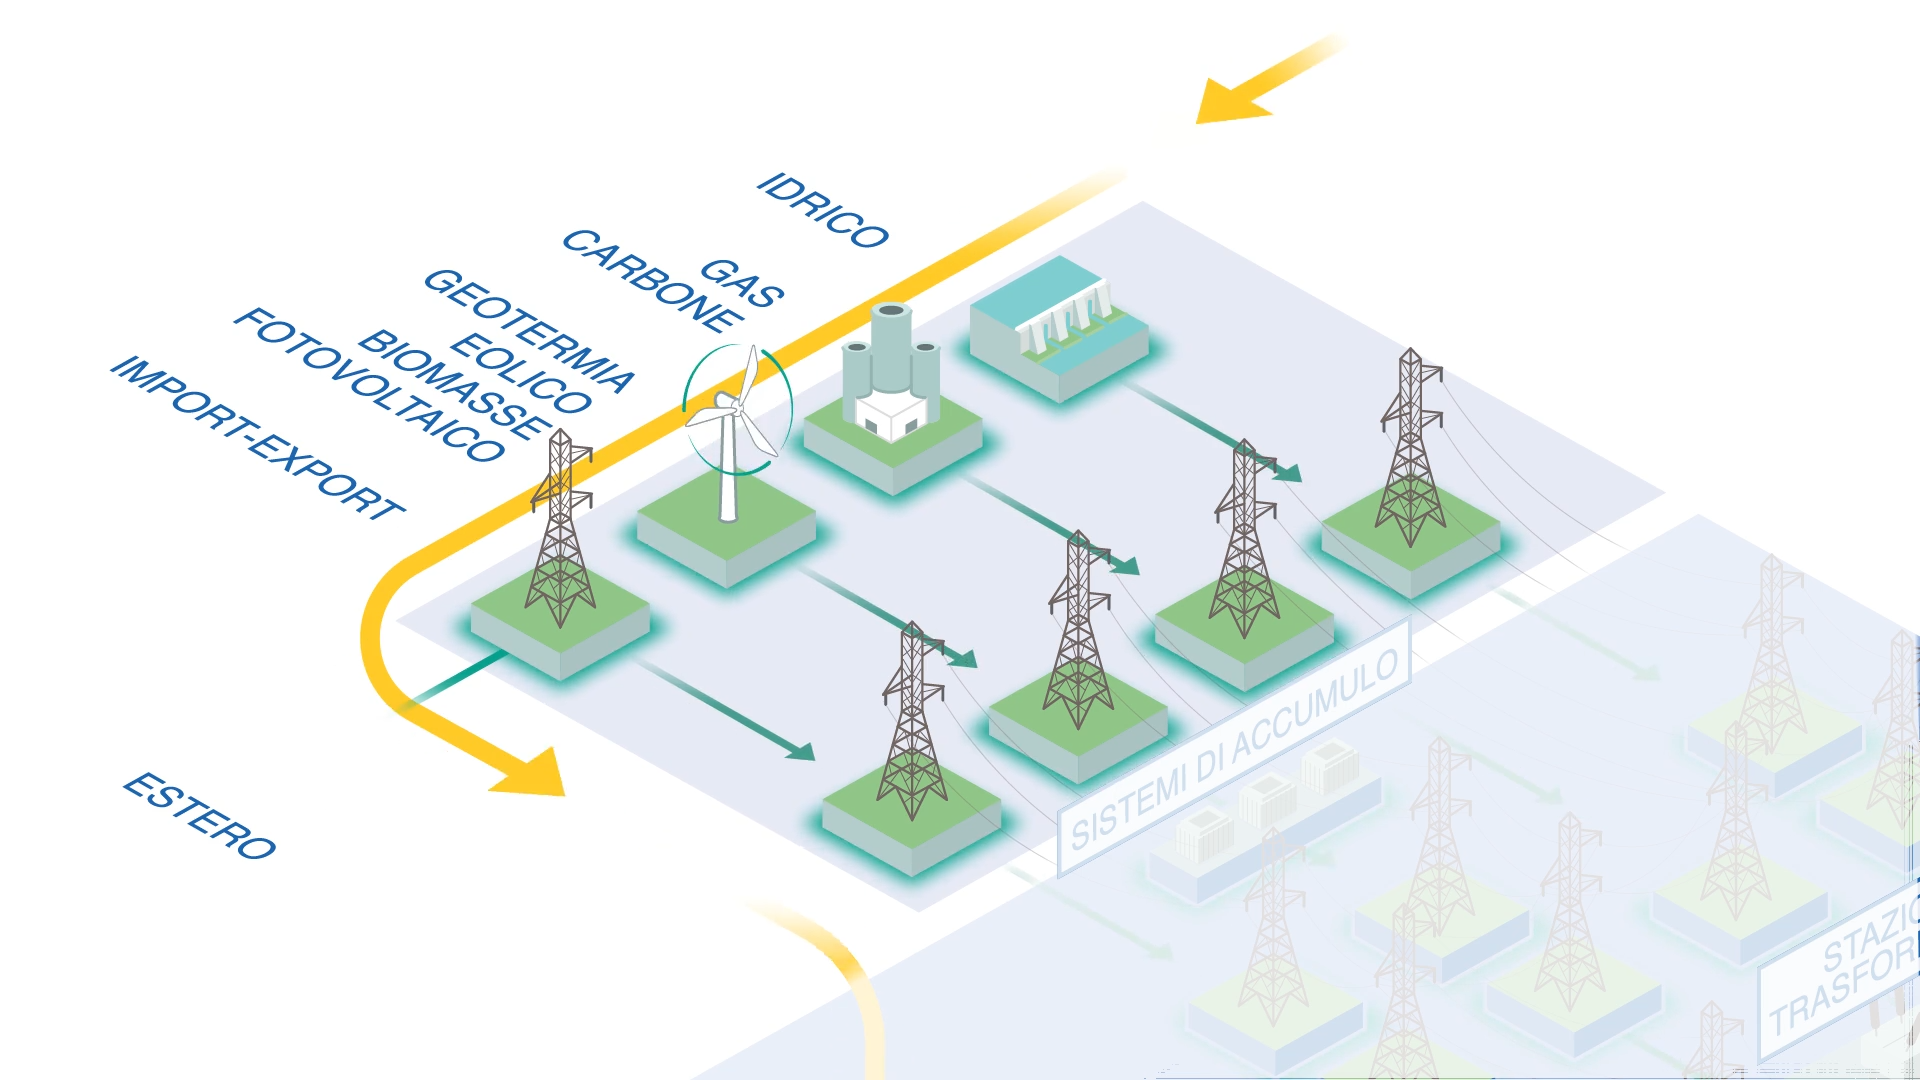
\includegraphics[width=0.45\linewidth]{img/Terna-Produzione.png}
    \caption{Fonte immagine: Terna - Produzione}
\end{figure}

% La produzione di elettricità, sia nel sistema tradizionale sia con l'utilizzo delle Smart Grid, avviene attraverso un mix energetico di Fonti Energetiche non Rinnovabili (\textbf{non FER}) e Fonti Energetiche Rinnovabili (\textbf{FER}).

% nuovo
La generazione di energia elettrica, sia nei sistemi tradizionali che nelle Smart Grid, si fonda su un mix energetico che bilancia Fonti Energetiche non Rinnovabili (non-FER) e Fonti Energetiche Rinnovabili (FER), Tabella \ref{tab:GSE-mix-nazionale-2023}. Questo equilibrio è un fattore chiave per la stabilità e la sostenibilità del sistema elettrico nazionale.
% fine nuovo

% Il mix energetico italiano sfrutta varie fonti tra cui le non FER, con circa il 54\%, e il restante 46\% proviene invece dalle fonti FER Tabella \ref{tab:GSE-mix-nazionale-2023}.

% \vspace{-0.4cm}
\begin{table}[h!]
    \renewcommand{\arraystretch}{1.4}
    \centering
    \begin{tabular}{lc}
        % \multicolumn{2}{c}{\shortstack{}}\\
         % \multicolumn{2}{c}{Fonti primarie utilizzate \%} \\
         \hline
         \textbf{Fonti primarie utilizzate}	& \textbf{\%} \\
         \hline
         Fonti rinnovabili & 46 \\
         Gas naturale& 43 \\
         Carbone& 5 \\
         Altre fonti & 5 \\
         Prodotti petroliferi& 1 \\
         \hline
    \end{tabular}
    \caption{Composizione del mix iniziale nazionale immessa nel anno 2023 \cite{GSE}}
    \label{tab:GSE-mix-nazionale-2023}
\end{table}

% \vspace{-0.4cm}


% \renewcommand{\arraystretch}{1.5}
% \begin{longtable}[!h]{p{5cm}p{0.5cm}}

        
%     \caption{Composizione del mix iniziale nazionale immessa nel anno 2023 \cite{GSE}}
%     \label{tab:GSE-mix-nazionale-2023}\\
    
%     \hline
%     \textbf{Fonti primarie utilizzate}	& \textbf{\%} \\
%     \hline
%     \endfirsthead
    
%     \hline
%     \textbf{Fonti primarie utilizzate}	& \textbf{\%} \\
%     \hline
%     \endhead
    
%          Fonti rinnovabili & 46 \\
%          Gas naturale& 43 \\
%          Carbone& 5 \\
%          Altre fonti & 5 \\
%          Prodotti petroliferi& 1 \\
    
%     \hline
% \end{longtable}



% \footnote{Non Trade adjusted - ovvero questi dati non sono stati corretti per import/export  }


% In particolare, come riportato nel "Rapporto Mensile sul Sistema Elettrico 2024" redatto da Terna \cite{TernaRapporto2024}, si mostra che l'assorbimento totale, la somma di produzione più importazioni di energia elettrica, nel periodo Gen-Dic 2024 è stata di $312\,TWh$, di cui FER \footnote{Produzione da FER = Idrico + Biomasse + Geotermico + Eolico + Fotovoltaico} $129\,TWh\,(49\,\%)$, non FER $132\,TWh\ (51\,\%)$ e importazioni $51\,TWh$ principalmente da Francia e Svizzera.

% nuovo
\newpage
Analizzando il contesto italiano, i dati più recenti del "Rapporto Mensile sul Sistema Elettrico" di Terna per il periodo Gennaio-Dicembre 2024 \cite{TernaRapporto2024} offrono un quadro preciso della situazione. A fronte di un assorbimento totale di energia elettrica di $312\,TWh$, la produzione nazionale netta si è attestata a $261\,TWh$. La composizione di tale produzione evidenzia un contributo quasi paritetico tra fonti rinnovabili e non rinnovabili. In particolare, $132\,TWh\ (51\,\%)$ della produzione è derivato da fonti non-FER, mentre $129\,TWh\,(49\,\%)$ è stato generato da FER, a testimonianza del progresso della transizione energetica. Il fabbisogno è stato infine completato da un saldo netto di importazioni dall'estero per $51\,TWh$, principalmente da Francia e Svizzera.
% fine nuovo



\begin{figure}[h!]
    \centering
    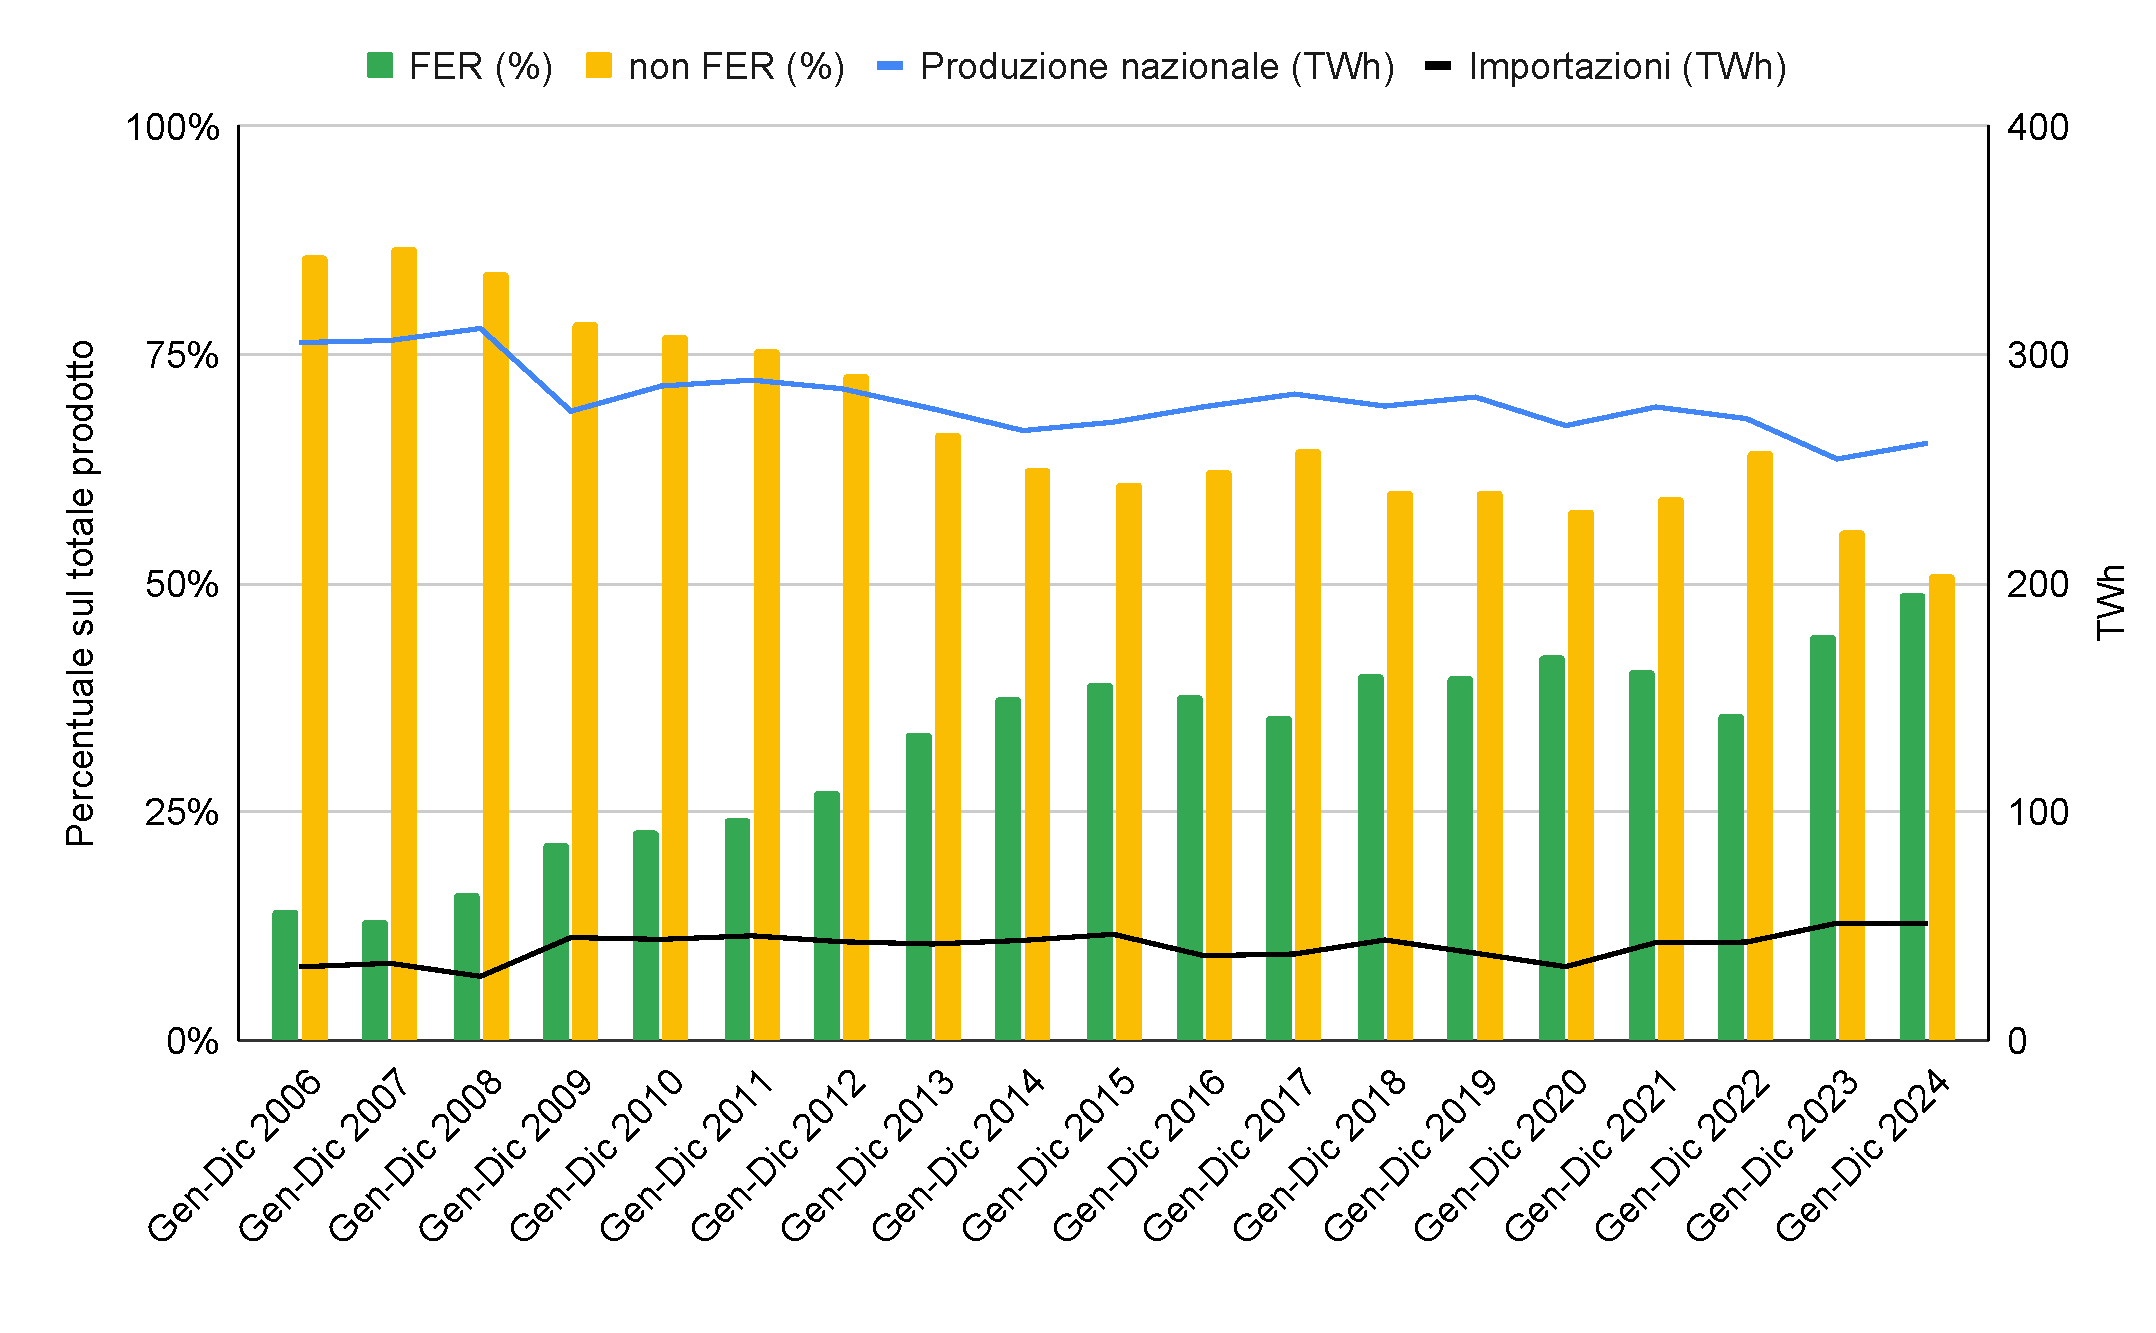
\includegraphics[trim= 0cm 1.5cm 0cm 0cm, clip, width=0.7\linewidth]{img/Terna-rapporto-annuale-2006-2024-v2.pdf}
    \caption{Produzione nazionale annuale suddivisa tra FER e non FER \cite{terna-rapporto-mensile-sito}}
    \label{graph:Terna-rapporto-annuale-2006-2024}
\end{figure}

% Si può vedere dal Grafico \ref{graph:Terna-rapporto-annuale-2006-2024} come dal 2006 al 2024 ci sia stato un incremento consistente della produzione di energia attraverso le fonti FER, arrivando quasi ad un break even nel 2024. In particolar modo, come si evince dal Grafico \ref{graph:Terna-FER-a-confronto-2006-2024}, questa crescita è stata possibile grazie all'installazione di pannelli fotovoltaici a partire dall'anno 2009 e il progressivo e costante aumento degli impianti eolici.


% nuovo
La crescente rilevanza delle fonti rinnovabili non è un fenomeno recente, ma il risultato di un trend consolidato. Come evidenziato nella Figura \ref{graph:Terna-rapporto-annuale-2006-2024}, il periodo dal 2006 al 2024 ha visto un incremento costante e significativo della produzione da FER, fino a raggiungere quasi un punto di pareggio con le fonti convenzionali nell'ultimo anno di rilevazione. L'analisi disaggregata di questa crescita, Figura \ref{graph:Terna-FER-a-confronto-2006-2024}, rivela che i principali motori di questa trasformazione sono stati l'espansione del settore fotovoltaico, a partire dal 2009, e lo sviluppo continuo e progressivo dell'energia eolica.
% fine nuovo

\begin{figure}[h!]
    \centering
    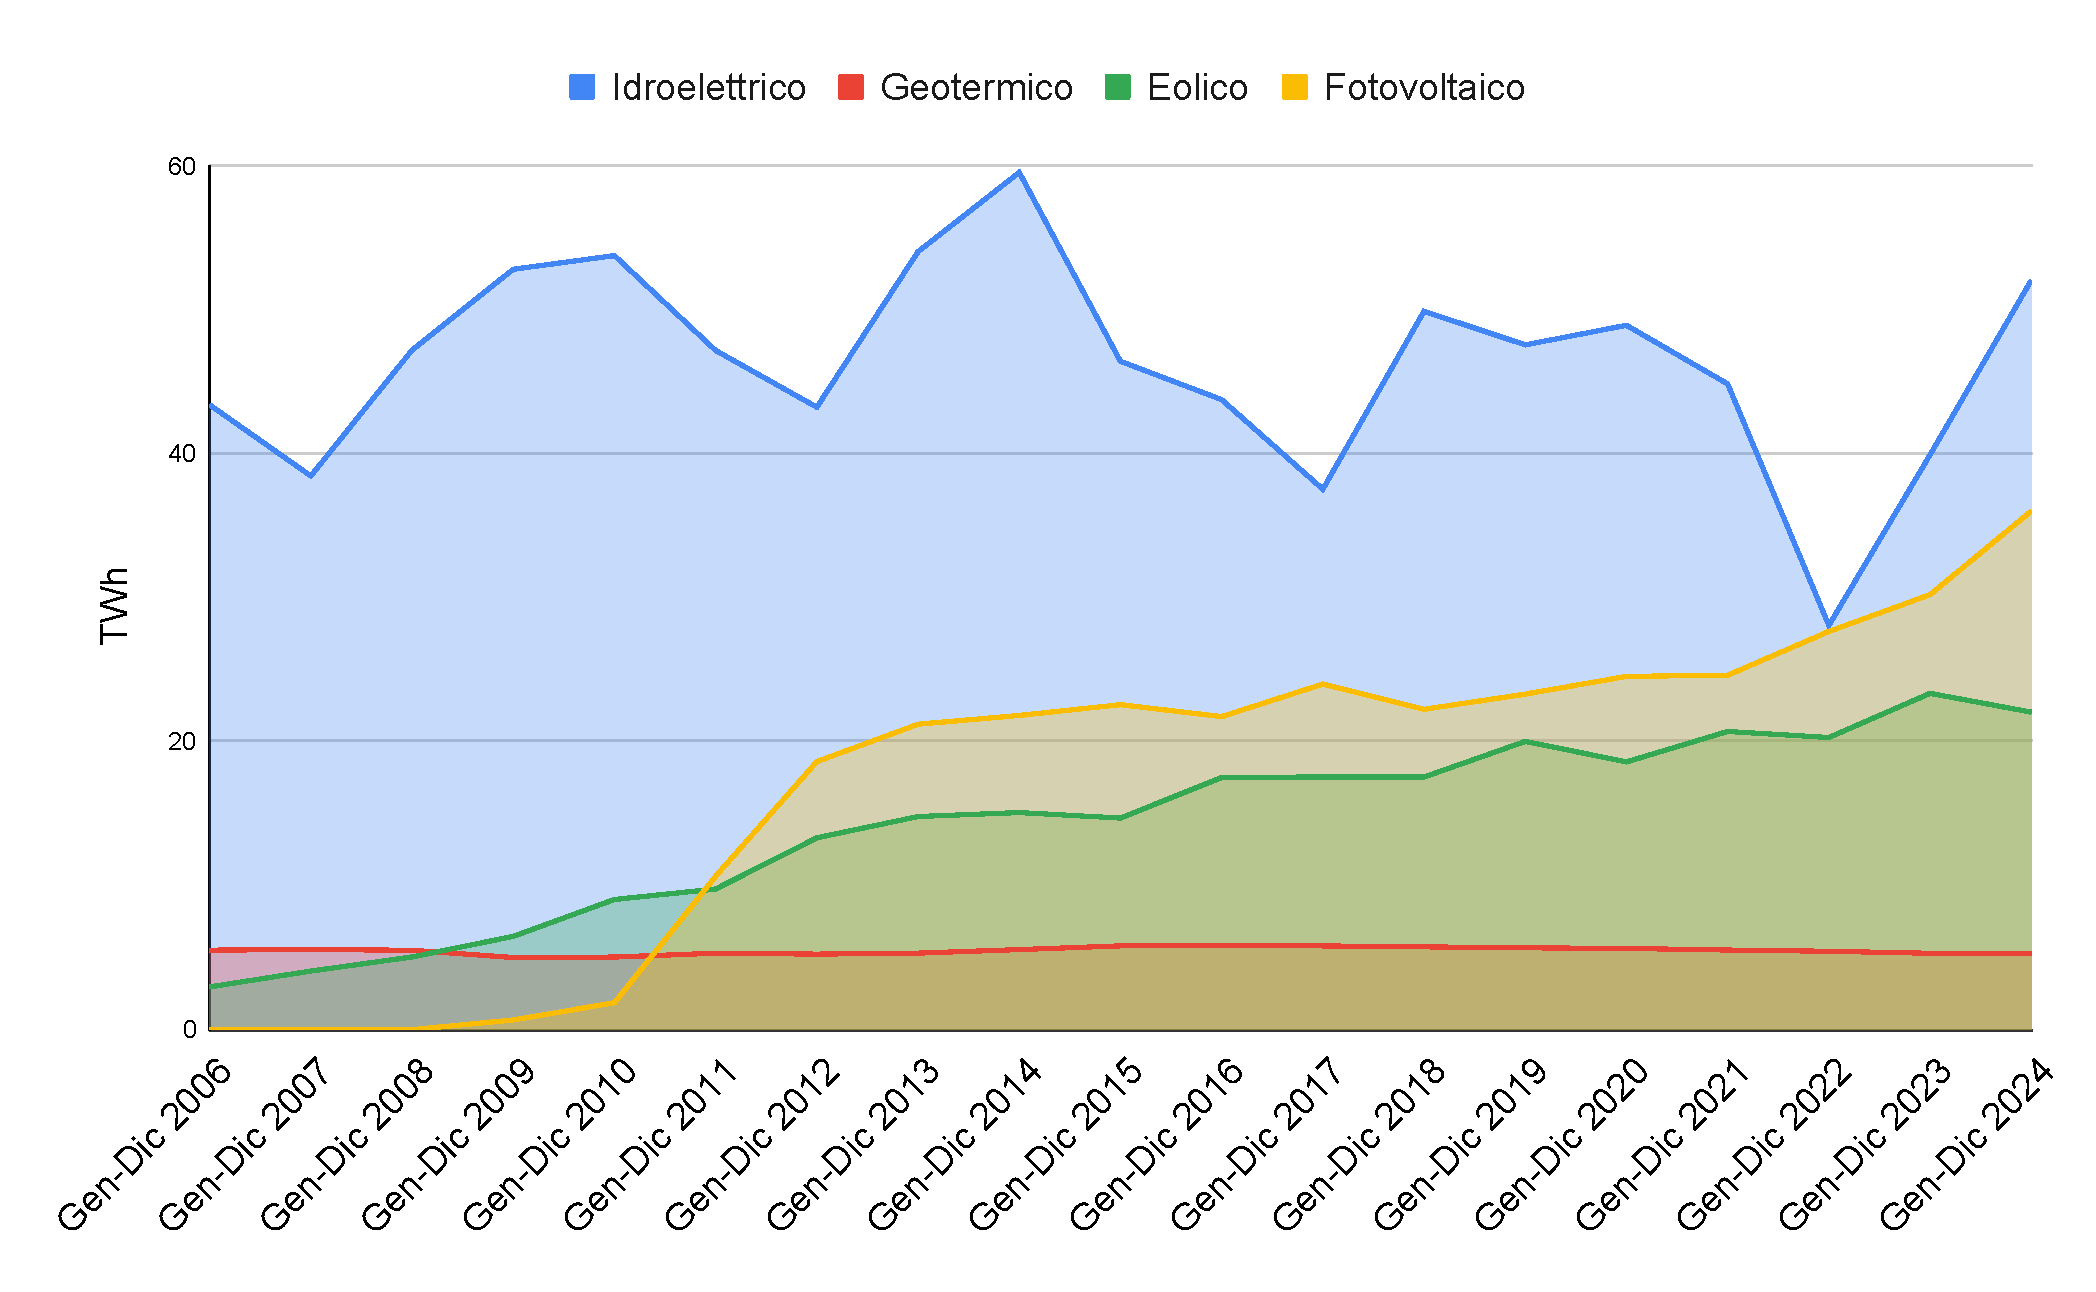
\includegraphics[trim= 0cm 1cm 0cm 1.05cm, clip, width=0.7\linewidth]{img/Terna-FER-a-confronto-2006-2024-v2.pdf}
    \caption{Suddivisione delle principali FER in Italia \cite{terna-rapporto-mensile-sito}}
    \label{graph:Terna-FER-a-confronto-2006-2024}
\end{figure}


\begin{figure}[b]
    \centering
    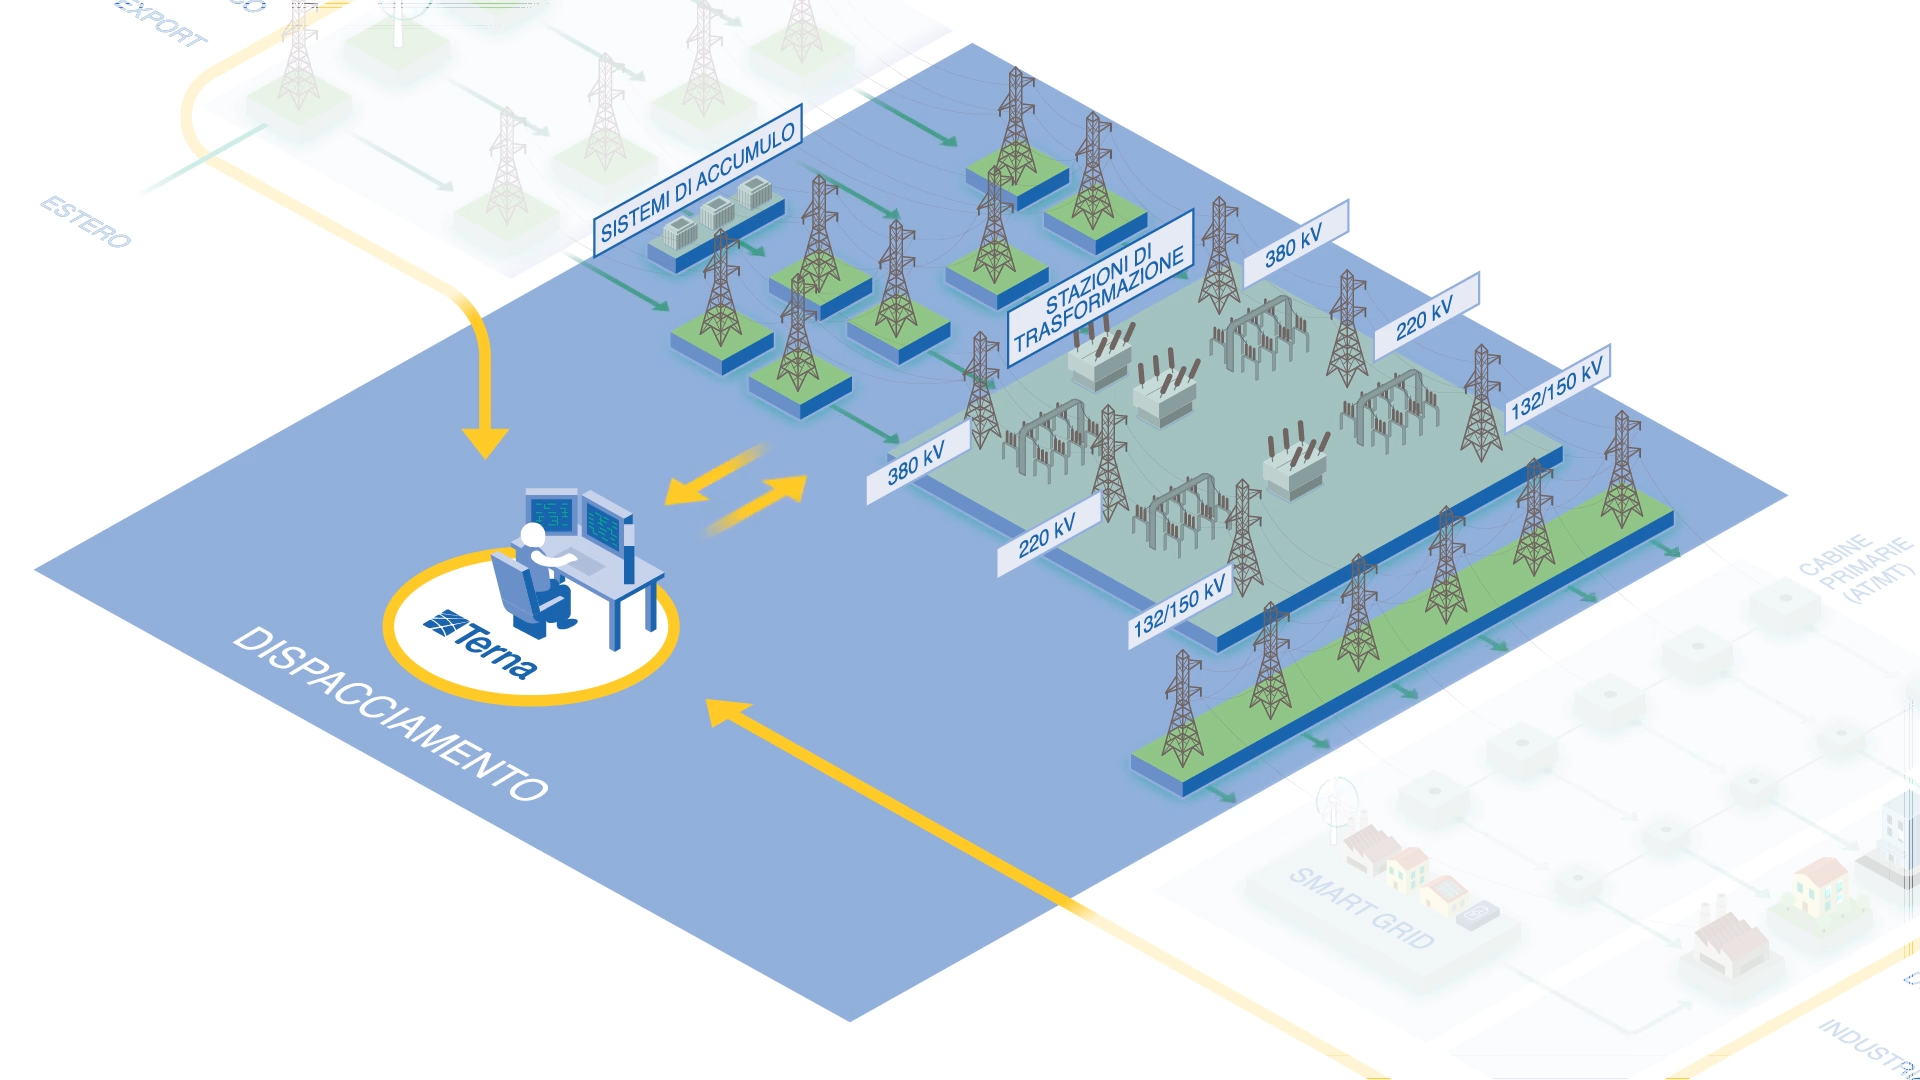
\includegraphics[width=0.5\linewidth]{img/Terna-Trasmissione.png}
    \caption{Fonte immagine: Terna - Trasmissione}
\end{figure}

\newpage
\subsection{La Trasmissione e il Dispacciamento dell'Energia}
% La società italiana che, in un regime di monopolio naturale, si occupa della trasmissione e del dispacciamento è Terna. Questa modalità di governance è diffusa anche nel resto d'Europa, poiché è la configurazione ideale da mantenere per garantire una gestione, un mantenimento e uno sviluppo costante su tutta la Rete Elettrica Nazionale (RTN).

La fase di trasmissione costituisce il sistema nervoso della rete elettrica, incaricata di trasportare l'energia su lunghe distanze, dalle centrali di produzione alle reti di distribuzione. In Italia, questa infrastruttura strategica, nota come Rete di Trasmissione Nazionale (RTN), è gestita in regime di monopolio naturale da Terna, che opera in qualità di \textit{Transmission System Operator} (TSO). Tale modello di governance, diffuso in gran parte d'Europa, è considerato ottimale per garantire l'efficienza, la sicurezza e lo sviluppo coordinato dell'intera infrastruttura elettrica nazionale.

% La trasmissione è un punto cruciale del dispacciamento dell'energia elettrica che comprende: 

% \begin{itemize}
%     \item il monitoraggio dei flussi energetici deviando l'energia nelle zone con più alto assorbimento
%     \item le procedure operative per il controllo coordinato di tutti i componenti sistemici
%     \item la programmazione di riparazioni, l'allaccio di nuove linee e l'indisponibilità di pezzi della rete
%     \item la previsione del fabbisogno energetico nazionale ora per ora
% \end{itemize}


\subsubsection{Funzioni del TSO: Il Dispacciamento}

Il ruolo di Terna non si limita alla manutenzione fisica della rete, ma include la complessa attività di dispacciamento: la gestione e il controllo in tempo reale dei flussi energetici per assicurare costantemente l'equilibrio tra energia prodotta e consumata. 

Le principali responsabilità del dispacciamento includono:

\begin{itemize}
    \item il \textbf{monitoraggio} continuo dei flussi di potenza e la loro deviazione per soddisfare i picchi di assorbimento regionali;
    \item l'attuazione di \textbf{procedure operative} per il controllo coordinato di tutti gli elementi del sistema (centrali, linee, stazioni);
    \item la \textbf{pianificazione} delle manutenzioni, dell'allacciamento di nuove linee e della gestione delle indisponibilità programmate o accidentali di porzioni della rete;
    \item la \textbf{previsione} del fabbisogno energetico nazionale con un dettaglio orario, fondamentale per la programmazione della produzione.
\end{itemize}


% Tutto questo tenendo sempre in considerazione che la sinusoide di rete, dalla produzione all'utente finale viene impiegata una corrente alternata, in tutta Italia - ed Europa - deve, in qualsiasi istante, avere una frequenza nominale ($f_n$) di $50\,Hz$ con possibile funzionamento senza limiti di tempo (condizioni normali) da $47,5\,Hz$ a $51,5\,Hz$, e una tensione nominale di rete, indicata con $U_n$, di $230\,V$ per le forniture monofase e $400\,V$ per le forniture trifase, con tolleranze di $\pm 10\,\%$ ovvero da $207\,V$ a $253\,V$ e da $360\,V$ a $440\,V$. \cite{Fase-di-rete-terna} \cite{CEI0-21}

% La sinusoide di rete utilizza corrente alternata dalla produzione all'utente finale. In tutta Italia ed Europa, questa deve mantenere parametri specifici in qualsiasi istante.


% La frequenza nominale ($f_n$) è di $50\,Hz$ . In condizioni normali, può funzionare senza limiti di tempo tra $47,5\,Hz$ e $51,5\,Hz$.\cite{Fase-di-rete-terna} 


% La tensione nominale di rete ($U_n$) è di $230\,V$ per le forniture monofase e $400\,V$ per le forniture trifase, con tolleranze ammesse di $\pm 10\,\%$ \cite{CEI0-21}, quindi:


% \begin{center}
%     Monofase: $207\,V$ a $253\,V$ e Trifase: $360\,V$ a $440\,V$
% \end{center}

% \begin{itemize}
%     \item[] Monofase: $207\,V$ a $253\,V$
%     \item[] Trifase: $360\,V$ a $440\,V$
% \end{itemize}




% Un, Vn soo differenti!


% Principalmente al livello di trasmissione si lavora ad Alta ed Altissima tensione, rispettivamente da $35\,kV < U \leq 220\,kV$ e oltre i $220\,kV$\cite{alta-tensione-parametri}. L'utilizzo di linee ad elevato potenziale è dettata dalla necessità di limitare la corrente su di esse e dunque ridurre drasticamente le perdite di energia per effetto Joule.



\subsubsection{Parametri Tecnici della Rete di Trasmissione}

Per garantire la stabilità e la qualità della fornitura, l'energia elettrica in corrente alternata deve rispettare parametri tecnici rigorosi in ogni punto della rete europea. I due principali indicatori sono la frequenza e la tensione.


\begin{itemize}
    \item \textbf{Frequenza}: La frequenza nominale ($f_n$) del sistema è fissata a $50\,Hz$. Deviazioni da questo valore indicano uno squilibrio tra produzione e consumo. In condizioni operative normali, la rete è progettata per funzionare a tempo indeterminato entro un intervallo di tolleranza compreso tra $47,5\,Hz$ e $51,5\,Hz$, con limiti eccezionali di breve durata fuori dalle precedenti soglie \cite{Fase-di-rete-terna} \cite{EN-50160}.
    \item \textbf{Tensione}: A livello di utenza finale, la tensione nominale ($U_n$) è di $230\,V$ per le forniture monofase e $400\,V$ per quelle trifase, con una tolleranza ammessa di $\pm 10\,\%$\footnote{Monofase: da $207\,V$ a $253\,V$ e Trifase: da $360\,V$ a $440\,V$} \cite{CEI0-21}. Tuttavia, per minimizzare le perdite di energia per effetto Joule ($P = R \cdot I^2$) durante il trasporto su lunghe distanze, la trasmissione avviene a livelli di tensione molto più elevati. 
    La RTN, infatti, opera prevalentemente in Alta Tensione (AT), tra $35\,kV$ e $220\,kV$, e in Altissima Tensione (AAT), oltre i $220\,kV$\cite{alta-tensione-parametri}.
\end{itemize}



\begin{figure}[b]
    \centering
    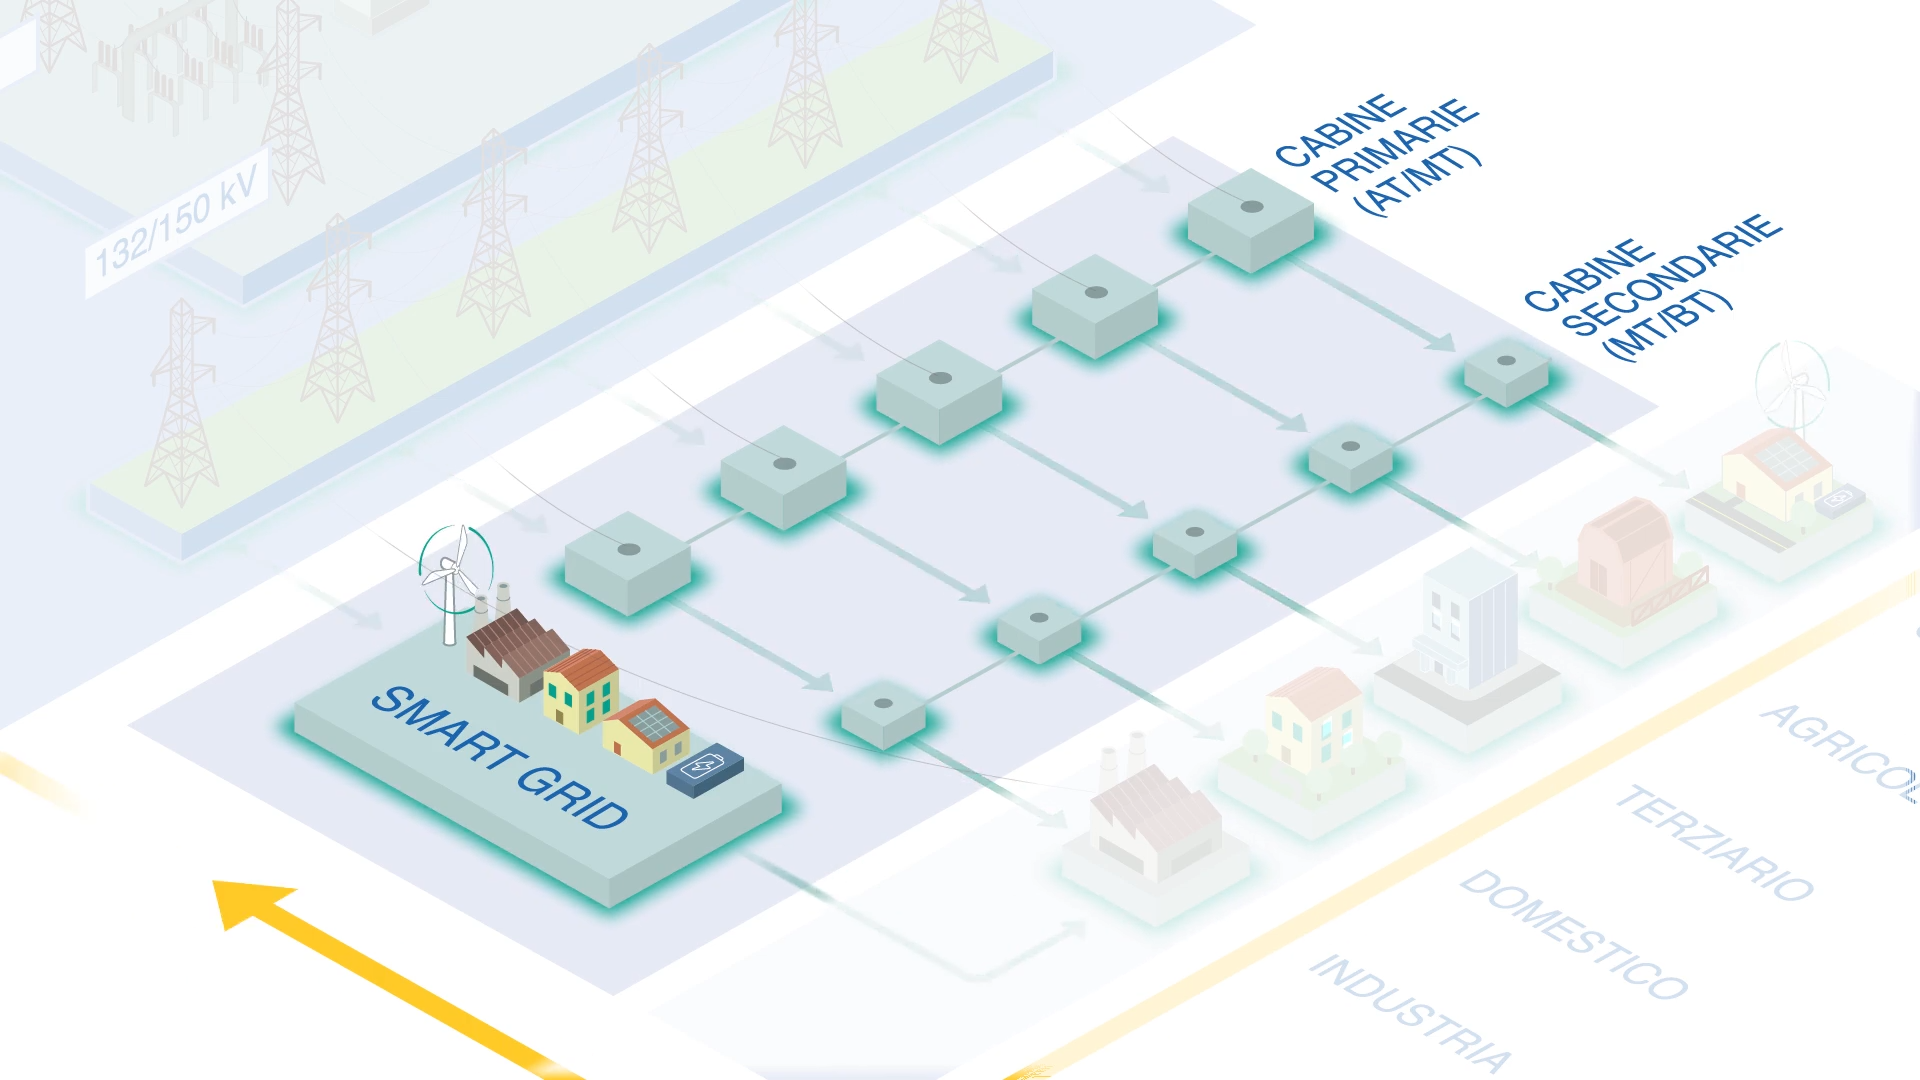
\includegraphics[width=0.5\linewidth]{img/Terna-Distribuzione.png}
    \caption{Fonte immagine: Terna - Distribuzione}
\end{figure}

\subsection{La Distribuzione dell'Energia}

% In Italia, se la trasmissione dell'energia elettrica è affidata a Terna tramite concessione statale, la distribuzione è invece gestita da diversi operatori attivi prevalentemente su base territoriale.

La fase di distribuzione rappresenta il segmento finale della filiera elettrica, con il compito di prelevare l'energia dalla Rete di Trasmissione Nazionale (RTN) e consegnarla capillarmente agli utenti finali. A differenza della trasmissione, gestita da un singolo operatore nazionale, Terna, il servizio di distribuzione in Italia è frammentato e liberalizzato, operato su base territoriale da diversi \textit{Distribution System Operator} (DSO).

% Attualmente sul territorio nazionale sono $114$ le aziende \cite{arera-distributori} che operano nel settore della distribuzione dell'energia elettrica

Attualmente, sul territorio nazionale operano circa 114 aziende di distribuzione \cite{arera-distributori}. Sebbene il numero sia elevato, il mercato è fortemente concentrato. I principali DSO, che servono collettivamente la quasi totalità della popolazione italiana, sono elencati in Tabella \ref{tab:dso_italia}, la quale riporta per ciascuno il gruppo di appartenenza, il numero di utenti e l'area geografica di competenza. Tra questi, spicca E-Distribuzione, società del gruppo Enel, che da sola gestisce oltre 31 milioni di utenze \cite{Clienti-sertivi-distribuzione}.

% I principali Distribution System Operator (DSO), che servono assieme la quasi totalità dei cittadini dell'intero territorio nazionale sono:

% \begin{itemize}
    
%     \item E-Distribuzione: società del Gruppo Enel con ben 31.1 milioni di utenti serviti  su tutto il territorio \cite{Clienti-sertivi-distribuzione}

%     \item Areti: società del Gruppo Acea con 2,8 milioni di utenti operante nei territori di Roma e Formello \cite{Clienti-sertivi-areti}

%     \item Unareti: società del Gruppo A2A con 1,2 milioni di utenti che gestisce i territori di Brescia, Milano e Bergamo \cite{Clienti-sertivi-uniareti}

%     \item Ireti: società del Gruppo Iren con  700 mila utenti serviti nei territori di Parma, Torino e Vercelli \cite{Clienti-sertivi-ireti}

%     \item Set Distribuzione: società del Gruppo Dolomiti Energia che serve il territorio della provincia autonoma di Trento con 330 mila utenze servite \cite{Clienti-sertivi-SetDistribuzione}

%     \item V-reti: società del Gruppo AGSM AIM nata dall'integrazione tra Servizi a Rete (SAR) e Megareti. Sono 279 mila le utenze servite nel territorio di Verona e Vicenza  \cite{Clienti-sertivi-v-reti}

%     \item InRete: società del Gruppo Hera distribuisce l'energia a oltre 264 mila utenti in Emilia-Romagna e in Toscana  \cite{Clienti-sertivi-edyna}

%     \item Edyna: società del Gruppo Alperia, nata nel 2016 dalla fusione di Azienda EnergeticaReti e SELNET, distribuisce l'energia nel territorio altoatesino servendo 240 mila utenti.\cite{Clienti-sertivi-edyna}
        
% \end{itemize}


\begin{table}[h!]
\renewcommand{\arraystretch}{1.5}
    \centering
    \begin{tabular}{ccclc}
        % \hline
        \hline
        \textbf{DSO} & \textbf{Gruppo di} & \textbf{Utenti Serviti} & \textbf{Principali} & \textbf{Fonti} \\
         & \textbf{Appartenenza} & \textbf{in mln.} & \textbf{aree geografiche} & \\
        \hline
        E-Distribuzione & Enel & 31,1 & Tutto il territorio nazionale & \cite{Clienti-sertivi-distribuzione} \\
        % \hline
        Areti & Acea & 2,8 & Roma e Formello & \cite{Clienti-sertivi-areti} \\
        % \hline
        Unareti & A2A & 1,2 & Brescia, Milano e Bergamo & \cite{Clienti-sertivi-uniareti} \\
        % \hline
        Ireti & Iren & 0,7 & Parma, Torino e Vercelli & \cite{Clienti-sertivi-ireti} \\
        % \hline
        Set Distribuzione & Dolomiti Energia & 0,3 & Provincia autonoma di Trento & \cite{Clienti-sertivi-SetDistribuzione} \\
        % \hline
        V-reti & AGSM AIM & 0,3 & Verona e Vicenza & \cite{Clienti-sertivi-v-reti} \\
        % \hline
        InRete & Hera & 0,3 & Emilia-Romagna e Toscana & \cite{Clienti-sertivi-InRete} \\
        % \hline
        Edyna & Alperia & 0,2 & Alto Adige & \cite{Clienti-sertivi-edyna} \\
        % \hline
        \hline
    \end{tabular}
    \caption{Principali Distributori di Energia Elettrica in Italia}
    \label{tab:dso_italia}
\end{table}


% Il distributore è responsabile del trasporto, della trasformazione e della consegna ad utenti finali e produttori dell'energia elettrica su reti in Media Tensione, da $1\,kV$ a $35\,kV$, e Bassa Tensione $<1kV$.
% L'energia elettrica viene prelevata dalla rete ad Alta Tensione (AT), da $35\,kV$ a $220\,kV$ \cite{alta-tensione-parametri}, e portata al livello di Media Tensione  all'interno delle Cabine Primarie, cioè $400\,V$ per sistemi trifase e $230\,V$ per sistemi monofase.


\subsubsection{Architettura della Rete di Distribuzione}


Il DSO è responsabile del trasporto, della trasformazione e della consegna dell'energia elettrica su reti in Media Tensione (MT), con tensioni tipicamente comprese tra $1\,kV$ e $35\,kV$, e in Bassa Tensione (BT), con tensioni inferiori a $1\,kV$.


Il processo di trasformazione della tensione avviene in più passaggi:


\begin{enumerate}
    \item Nelle Cabine Primarie, l'energia viene prelevata dalla rete di trasmissione in Alta Tensione (AT) e trasformata a un livello di Media Tensione (es. $15\,kV$ o $20\,kV$). Queste cabine fungono da nodo di interconnessione tra la rete del TSO e quella del DSO.
    \item L'energia in Media Tensione viene quindi distribuita attraverso una rete di cavi (spesso interrati nei centri urbani) fino a raggiungere le Cabine Secondarie.
    \item All'interno delle Cabine Secondarie, un ulteriore trasformatore abbassa la tensione da Media a Bassa Tensione, portandola ai valori standard per l'utenza finale: $400\,V$ per le forniture trifase e $230\,V$ per quelle monofase.
\end{enumerate}


\subsection{Le Utenze Finali: da Consumatori Passivi a Nodi Attivi della Rete}


% Gli utenti finali possono scegliere il proprio venditore di energia elettrica in base alle specifiche esigenze e alle offerte di mercato.

% Molto utile può essere infatti l'utilizzo de \href{https://www.ilportaleofferte.it/portaleOfferte/}{"Il portale delle offerte"} \footnote{https://www.ilportaleofferte.it/portaleOfferte/} messo a disposizione proprio da ARERA \footnote{Autorità di Regolazione per Energia Reti e Ambiente}.
% % Questo comparatore fornisce all'utente finale una panoramica chiara di tutte le offerte disponibili sul mercato, questo per poter fare una scelta consapevole.
% Il comparatore permette agli utenti di visualizzare tutte le offerte disponibili sul mercato, consentendo loro di effettuare scelte informate e adatte alle proprie esigenze.



Nell'architettura della Smart Grid, il ruolo dell'utente finale subisce una profonda trasformazione, evolvendo da semplice consumatore passivo a nodo attivo e interattivo dell'ecosistema energetico. Se nel mercato tradizionale la scelta si limita alla selezione di un venditore di energia – un processo oggi facilitato da strumenti istituzionali come \href{https://www.ilportaleofferte.it/portaleOfferte/}{"Il portale delle offerte"}\footnote{https://www.ilportaleofferte.it/portaleOfferte/} di ARERA – nella Smart Grid l'utente diventa un partecipante dinamico grazie a nuove tecnologie e funzionalità.


Questa evoluzione è abilitata principalmente da due fattori:

\begin{enumerate}
    \item \textbf{Le Infrastrutture di Misurazione Avanzata} (AMI): attraverso i contatori intelligenti (\textit{Smart Meter}), i DSO possono non solo raccogliere i dati di consumo in tempo reale, ma anche inviare segnali di prezzo o comandi di gestione all'utente, creando un canale di comunicazione bidirezionale.
    
    \item \textbf{L'Emergere del "\textit{Prosumer}"}: come anticipato nella Sezione \ref{prosumer}, gli utenti dotati di impianti di generazione distribuita (es. fotovoltaico) possono produrre e immettere energia in rete, invertendo il flusso tradizionale di potenza e interagendo attivamente con il sistema.
\end{enumerate}


Inoltre, l'utente può ottimizzare i propri consumi attraverso sistemi di gestione dei carichi (\textit{Demand Response}) e dispositivi di automazione domestica come gli \textit{Home Energy Management Systems} (HEMS).


Questa crescente digitalizzazione e interconnessione del dominio utente, se da un lato promette maggiore efficienza e sostenibilità, dall'altro introduce nuove superfici di attacco e significative sfide di sicurezza informatica. La compromissione di \textit{Smart Meter}, HEMS o altri dispositivi connessi potrebbe infatti avere ripercussioni non solo sul singolo utente, ma sulla stabilità dell'intera rete di distribuzione.



\begin{figure}[h!]
    \centering
    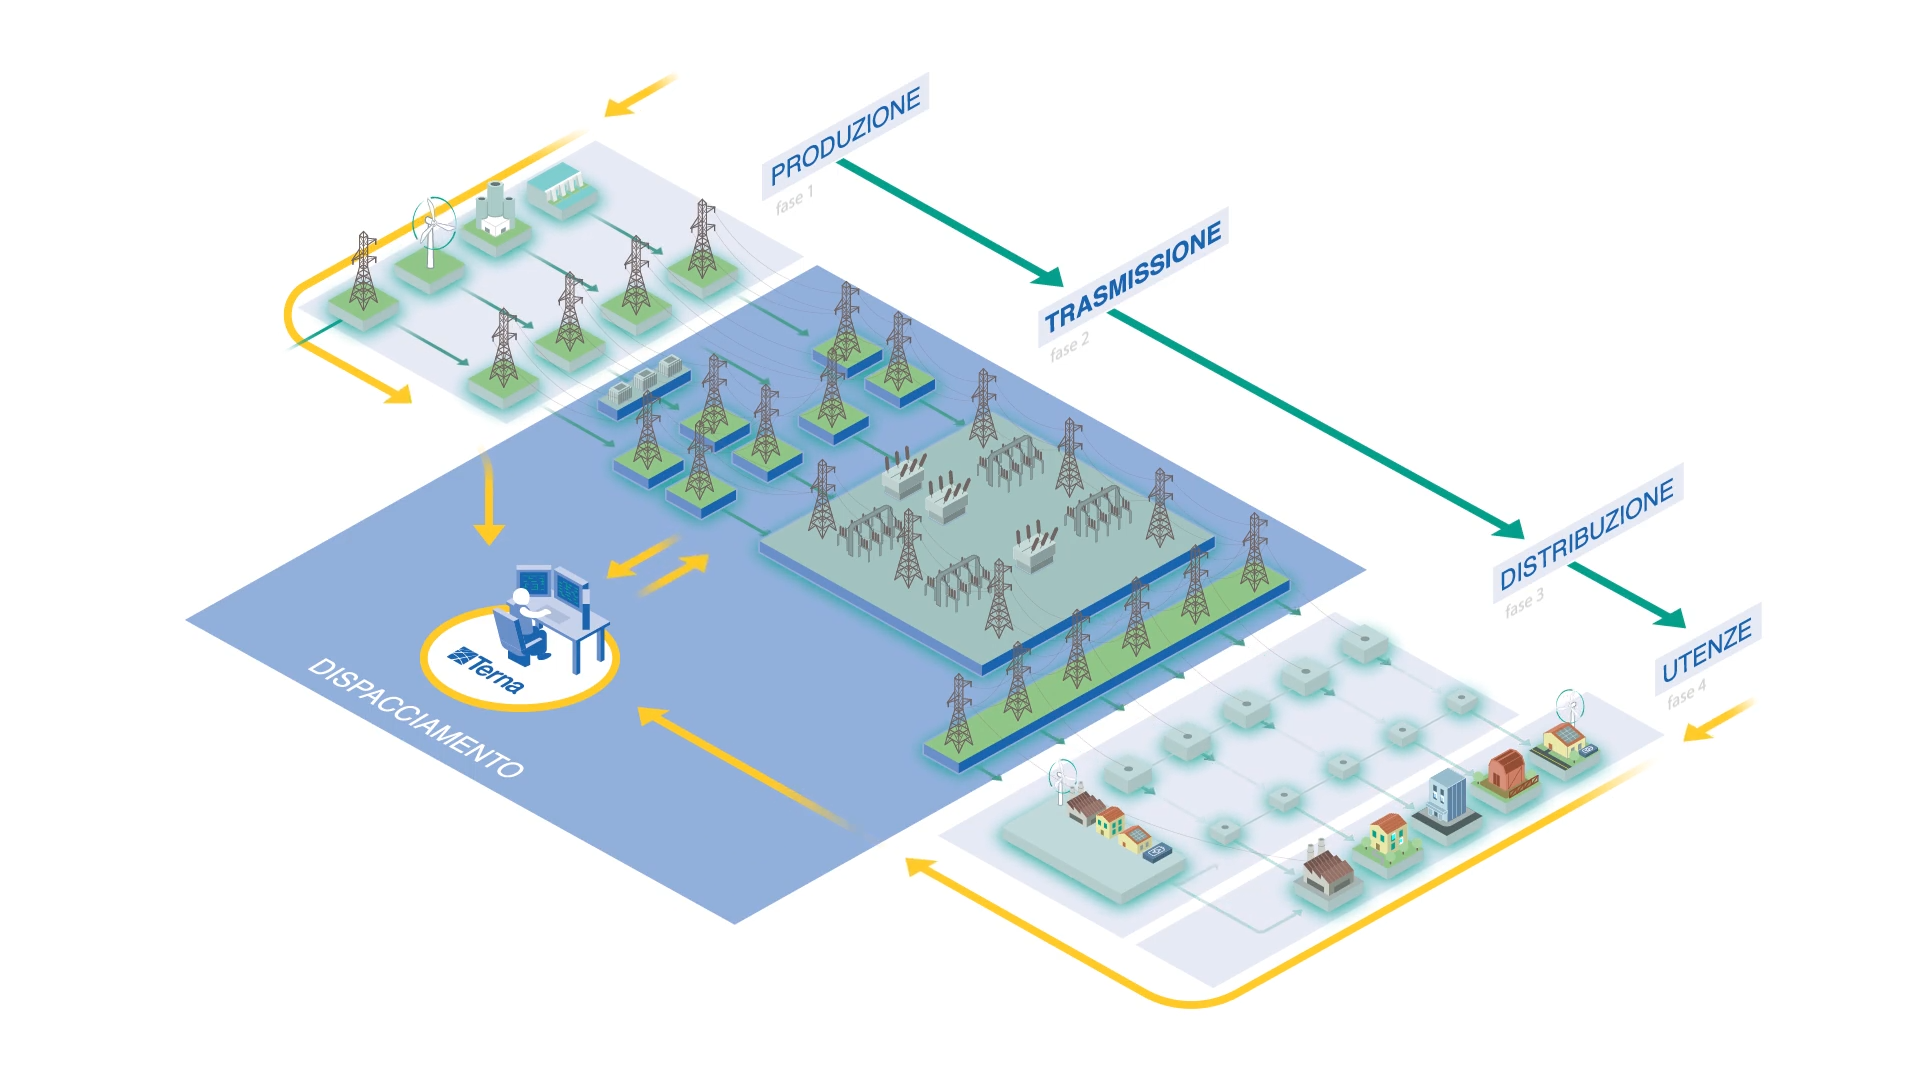
\includegraphics[trim= 6.5cm 0cm 6cm 0cm, clip,width=1\linewidth]{img/Terna-Sistema-Elettrico.png}
    \caption{Fonte immagine: Terna - Sistema Elettrico}
\end{figure}




\chapter{Il paradigma tecnologico del Cloud Computing e i suoi principali vantaggi}
\label{allegato:Secondo-allegato}


% Questa sezione di approfondimento si propone di esplorare come l'adozione di paradigmi cloud stia trasformando le infrastrutture della rete intelligente. Inizialmente, verranno introdotti i concetti fondamentali del Cloud Computing e i suoi principali vantaggi in termini di flessibilità, resilienza ed efficienza. 


\section{Introduzione al Cloud Computing}

% Da almeno due decenni il nome \textit{Cloud Computing} ha iniziato a diffondersi a profusione, con una crescita significativa data grazie a piattaforme come Amazon Web Service (AWS), Google Cloud Platform (GCP) e Azure la piattaforma cloud di Microsoft.

Negli ultimi due decenni, il \textit{Cloud Computing} si è affermato come il paradigma dominante per l'erogazione di servizi informatici, una transizione accelerata dalla maturità di piattaforme leader come Amazon Web Services (AWS), Microsoft Azure e Google Cloud Platform (GCP).


Formalmente, il \textit{National Institute of Standards and Technology} (NIST) definisce il \textit{Cloud Computing} come "un modello per abilitare un accesso di rete \textit{on-demand}, conveniente e ubiquo a un pool condiviso di risorse di calcolo configurabili (es. reti, server, storage, applicazioni e servizi) che possono essere rapidamente approvvigionate e rilasciate con un minimo sforzo di gestione o interazione con il fornitore di servizi" \cite{NIST-cloud-computer}


% Con il termine \textit{Cloud Computing}, si intende la fruizione di servizi quali: software, informazioni, intere infrastrutture di server ecc., utilizzando internet ("Il Cloud"). Eliminando la necessità per gli individui e le aziende di autogestire le risorse fisiche.
% e di pagare solo per ciò che utilizzano.

In termini più semplici, il \textit{Cloud Computing} permette a organizzazioni e individui di accedere a risorse IT via Internet ("\textit{il Cloud}"), astraendo la complessità della gestione fisica e logica dell'infrastruttura sottostante. L'analogia più calzante, particolarmente pertinente per questa tesi, è quella con la rete elettrica pubblica: un'azienda non ha bisogno di costruire e mantenere la propria centrale elettrica privata per alimentare le proprie attività. Al contrario, si connette alla rete nazionale e paga solo per l'energia effettivamente consumata (modello \textit{pay-per-use}).



% Un paragone vicino alla vita concreata di tutti i giorni, sempre restando a tema, è pensare al Cloud Computing come l'energia elettrica. Non si hai bisogno di costruire una centrale elettrica, non deve assumere tecnici per mantenerla funzionante 24 ore su 24 con tutti i parametri visti in precedenza, e non si paga un costo fisso enorme se si consuma poco. Bensì si paga una quota per delegare a qualcun altro tutto il lavoro, l'efficientamento, la flessibilità e la sicurezza dell'intero sistema.

Allo stesso modo, il \textit{Cloud Computing} consente di delegare a un fornitore specializzato la gestione, la manutenzione, la sicurezza e la scalabilità dell'infrastruttura IT, trasformando un ingente costo fisso iniziale (CAPEX)\footnote{\textit{Capital Expenditure}: rappresentano flussi di cassa in uscita per la realizzazione di investimenti in attività immobilizzate di natura operativa. \cite{borsa-italiana-CAPEX}} in un costo operativo variabile (OPEX)\footnote{\textit{Operating Expenses}: è un costo che un'azienda sostiene attraverso le sue normali attività, incluse spese come l'affitto che sono tipicamente deducibili dalle tasse. \cite{opex}}, proporzionale all'utilizzo effettivo delle risorse.




\subsection{Modelli di Deployment del Cloud Computing}

% Troviamo principalmente due tipologie di modelli\footnote{In realtà ne esisterebba pure una terza: \textit{Hybrid Cloud}, ma non trattata} per il \textit{Deploy} di un Cloud Computing \cite{GCP}.

La scelta di un'architettura \textit{cloud} dipende dalle specifiche esigenze di un'organizzazione in termini di sicurezza, controllo, scalabilità e costi. Secondo la classificazione del NIST \cite{NIST-cloud-computer}, esistono quattro principali modelli di \textit{deployment} (o implementazione) del \textit{cloud}.

\subsubsection{Public Cloud}

% I \textit{Public Cloud} sono aziende di terze parti che possiede l'infrastruttura e si occupa di mantenere l'infrastruttura aggiornata, sicura ed efficiente. Un esempio sono i Cloud Provider sopra citati: AWS, Google Cloud Platform e Azure, sicuramente i più famosi.
% Il loro core business è dunque vendere il servizio cloud.


L'infrastruttura \textit{cloud} è di proprietà di un fornitore terzo (\textit{Cloud Service Provider} - CSP), come AWS, Microsoft Azure o GCP, che la rende disponibile al pubblico generale via Internet. In questo modello, le risorse (calcolo, \textit{storage}, rete) sono condivise tra più clienti (\textit{multi-tenancy}), sebbene logicamente isolate. Il cliente non ha alcuna visibilità o controllo sull'infrastruttura fisica, ma beneficia di un'enorme scalabilità, di un modello di costo \textit{pay-per-use} e della delega totale della gestione hardware al provider.


\subsubsection{Private Cloud}

% I \textit{Private Cloud} sono invece le singole organizzazione che provvedono a tutto: costruire, mantenere e migliorare il loro servizio cloud ed \textit{Hostarlo} nei loro Data Center.

L'infrastruttura \textit{cloud} è utilizzata in modo esclusivo da una singola organizzazione. Può essere di proprietà, gestita e operata dall'organizzazione stessa (\textit{on-premise}s) oppure da una terza parte, e può essere ospitata sia internamente che esternamente. Il vantaggio principale del \textit{Private Cloud} è il maggiore controllo sulla sicurezza, sulla governance dei dati e sulla personalizzazione dell'infrastruttura, pur mantenendo i benefici tipici del \textit{cloud} come l'automazione e l'elasticità delle risorse.


% Il loro core business non è vendere il servizio bensì di proteggere al più possibile i dati da esterni.

\subsubsection{\textit{Hybrid Cloud}}
Questo modello combina due o più infrastrutture \textit{cloud} distinte (\textit{private}, \textit{community} o \textit{public}) che rimangono entità uniche ma sono legate insieme da tecnologie standardizzate che permettono la portabilità di dati e applicazioni (es. "\textit{cloud bursting}" per la gestione dei picchi di carico). Un'organizzazione potrebbe, ad esempio, mantenere i dati sensibili su un \textit{Private Cloud} e utilizzare un \textit{Public Cloud} per le applicazioni meno critiche o per gestire carichi di lavoro variabili, ottenendo un equilibrio tra controllo e flessibilità.


\subsubsection{\textit{Community Cloud}}
L'infrastruttura \textit{cloud} è condivisa da diverse organizzazioni che hanno interessi comuni (es. requisiti di sicurezza, policy, conformità normativa). Può essere gestita dalle organizzazioni stesse o da una terza parte. Un esempio potrebbe essere un \textit{cloud} condiviso da diverse agenzie governative o da aziende dello stesso settore industriale (es. finanziario, sanitario o energetico) per ridurre i costi pur mantenendo standard di sicurezza elevati.


\subsection{Tecnologie Abilitanti per le Architetture Cloud-Native}

% Dopo aver toccato i diversi tipi di \textit{Deploy}, possiamo accennare le diverse tipologie utilizzate nell'ambito di applicazioni Cloud Native, questo anche per presentare le tecnologie utilizzate in seguito.

La transizione verso il \textit{Cloud Computing} non riguarda solo dove le applicazioni vengono eseguite, ma anche come vengono progettate, "impacchettate" e gestite. Le architetture \textit{Cloud-Native} si basano su un insieme di tecnologie che consentono di costruire sistemi resilienti, scalabili e flessibili. Di seguito viene presentata la traiettoria evolutiva di queste tecnologie, che saranno richiamate nell'analisi dell'architettura Smart Grid proposta.

% \begin{enumerate}
%     \item \textbf{\textit{Virtual Machine}}: l'utilizzo di VM è il primo approccio, il più semplice e veloce per utilizzare un infrastruttura Cloud. Questo è possibile grazie al fatto che l'applicazione che si vuole rendere fruibile attraverso il Cloud non dovrà subire modifiche di codice.

%     \item \textbf{\textit{Container}}: L'utilizzo di un gestore di Container, quale Docker o Containerd, permette di avere applicazioni isolate tra loro rispetto all'infrastruttura sottostante, ma soprattutto meno \textit{Resource Intensive} rispetto alle VM. Questa tecnologia sta alla base della nuova frontiera dei microservizi.

%     \item \textbf{\textit{Piattaforma di orchestrazione}}: Lo \textit{Stato dell'Arte} per l'utilizzo di cloud prevede di utilizzare Kubernetes come piattaforma che automatizza il deployment, la scalabilità e la gestione di applicazioni containerizzate.
% \end{enumerate}

\begin{enumerate}
    \item \textbf{Virtualizzazione tramite Virtual Machine (VM)} \\ La virtualizzazione tradizionale, basata su \textit{Virtual Machine} (VM), è stato il primo passo per astrarre l'hardware fisico. Una VM emula un intero computer, includendo un sistema operativo ospite (\textit{Guest OS}) completo, che viene eseguito sopra un \textit{hypervisor}. Questo approccio, noto come \textit{Infrastructure as a Service} (IaaS), offre un eccellente isolamento e permette di migrare applicazioni \textit{legacy} ("\textit{lift-and-shift}") nel \textit{cloud} con poche o nessuna modifica. Tuttavia, ogni VM comporta un significativo \textit{overhead} di risorse, poiché deve caricare un intero sistema operativo, risultando in tempi di avvio più lenti e una minore densità di applicazioni per host fisico.
    
    \item \textbf{Containerizzazione}\\La containerizzazione rappresenta un passo evolutivo verso una maggiore efficienza e portabilità. A differenza delle VM, un container non emula l'hardware, ma virtualizza il sistema operativo. Tutti i container in esecuzione su un \textit{host} condividono lo stesso kernel del sistema operativo ospitante (\textit{Host OS}), "impacchettando" solo l'applicazione e le sue dipendenze (librerie, file di configurazione). Tecnologie come Docker e containerd hanno reso questo approccio popolare. I vantaggi sono notevoli:
    
    \begin{itemize}
        \item \textbf{Efficienza:} Avendo un \textit{overhead} minimo, i container sono leggeri, si avviano in pochi secondi e consentono una maggiore densità di \textit{deployment}.
        \item \textbf{Portabilità:} Un container funziona in modo identico su qualsiasi ambiente che supporti un \textit{container runtime}, dal laptop dello sviluppatore al \textit{cloud} pubblico.
        \item \textbf{Abilitazione dei Microservizi:} La leggerezza e l'isolamento dei container li rendono la tecnologia ideale per implementare architetture a microservizi, dove un'applicazione complessa viene scomposta in piccoli servizi indipendenti e autonomi.
    \end{itemize}
    
    \item \textbf{Orchestrazione di Container con Kubernetes}\\Se i container risolvono il problema di come impacchettare e distribuire un'applicazione, l'orchestrazione risolve il problema di come gestirne centinaia o migliaia in un ambiente di produzione. Kubernetes (K8s) è diventata la piattaforma di orchestrazione \textit{de facto}. Essa automatizza il ciclo di vita delle applicazioni containerizzate, gestendo compiti complessi come:
    
    \begin{itemize}
        \item \textbf{Deployment e Scaling:} Distribuisce i container sui nodi di un cluster e ne scala automaticamente il numero in base al carico.
        \item \textbf{Service Discovery e Load Balancing:} Espone i container come servizi di rete e distribuisce il traffico tra di essi.
        \item \textbf{Self-healing:} Riavvia automaticamente i container che si bloccano, li sostituisce e gestisce i \textit{failover} \footnote{si intende la tecnica che prevede in caso di guasto o interruzione anomala nel funzionamento di un server, un componente hardware o una rete, la commutazione automatica a una struttura analoga ridondante o in \textit{standby} \cite{wikipedia-failover}}.
    \end{itemize}
\end{enumerate}

Kubernetes è il pilastro delle moderne applicazioni \textit{Cloud-Native}, fornendo l'automazione e la resilienza necessarie per operare sistemi distribuiti su larga scala.



\subsection{Principali Vantaggi del Cloud Computing}

% Questa fruizione di servizi, che tutti noi utilizziamo nel quotidiano, offre molti vantaggi tra cui una rapida espansione innovativa, una flessibilità enorme delle risorse ed economia di scala mai vista prima, sicurezza informatica e nel caso di \textit{Disaster Recovery} ed efficienza generale.

% Tipicamente questi servizi si pagano con la formula "Pay-per-Use", ovvero pagare solo le risorse effettivamente utilizzate, aiutando le aziende o privati ad avere costi operativi più bassi, con un infrastruttura più efficiente e scalare con il mutare delle esigenze \cite{Azure}.

L'adozione del \textit{Cloud Computing} offre vantaggi strategici che ne hanno guidato la rapida diffusione. I principali possono essere riassunti come segue \cite{Azure}:

\begin{itemize}
    \item \textbf{Efficienza Economica:} Sostituisce i grandi investimenti iniziali in hardware (CAPEX) con costi operativi variabili (OPEX), basati su un modello a consumo (\textit{pay-as-you-go}). Questo, unito alle economie di scala dei provider, riduce significativamente i costi totali dell'IT.
    \item \textbf{Agilità e Scalabilità:} Le risorse possono essere approvvigionate in pochi minuti e scalate automaticamente (elasticità) per rispondere in tempo reale alle fluttuazioni del carico di lavoro. Ciò accelera l'innovazione e garantisce prestazioni ottimali.
    \item \textbf{Affidabilità e Sicurezza:} I provider cloud offrono infrastrutture globali con elevati livelli di ridondanza, garantendo alta affidabilità e semplificando le strategie di \textit{Disaster Recovery} . Inoltre, investono in misure di sicurezza avanzate che superano le capacità della maggior parte delle singole organizzazioni.
\end{itemize}

In sintesi, il cloud permette alle aziende di delegare la complessità della gestione infrastrutturale per concentrarsi sul proprio core business, beneficiando di un'infrastruttura più efficiente, scalabile e sicura.




% \chapter{Approfondimenti}

% Magari approfondire:

% \begin{itemize}
%     \item https://static.ceinorme.it/strumenti-online/doc/18309.pdf - CEI 0-21 fase rete BT ecc
%     \item \url{https://download.terna.it/terna/Capitolo%201_Nuova%20sezione%201C_8d787c66135589d.pdf} ACCESSO ALLA RETE DI TRASMISSIONE NAZIONALE - TERNA - generatori

%     \item \url{https://www.e-distribuzione.it/content/dam/e-distribuzione/documenti/Piano%20di%20Sviluppo%202025.pdf} pagina 27
% \end{itemize}

% \section{Titolo}
% Lorem ipsum dolor sit amet, consectetur adipiscing elit. Donec sed nunc orci. Aliquam nec nisl vitae sapien pulvinar dictum quis non urna. Suspendisse at dui a erat aliquam vestibulum. Quisque ultrices pellentesque pellentesque. Pellentesque egestas quam sed blandit tempus. Sed congue nec risus posuere euismod. Maecenas ut lacus id mauris sagittis egestas a eu dui. Class aptent taciti sociosqu ad litora torquent per conubia nostra, per inceptos himenaeos. Pellentesque at ultrices tellus. Ut eu purus eget sem iaculis ultricies sed non lorem. Curabitur gravida dui eget ex vestibulum venenatis. Phasellus gravida tellus velit, non eleifend justo lobortis eget. 

% \subsection{Sottotitolo}
% Lorem ipsum dolor sit amet, consectetur adipiscing elit. Donec sed nunc orci. Aliquam nec nisl vitae sapien pulvinar dictum quis non urna. Suspendisse at dui a erat aliquam vestibulum. Quisque ultrices pellentesque pellentesque. Pellentesque egestas quam sed blandit tempus. Sed congue nec risus posuere euismod. Maecenas ut lacus id mauris sagittis egestas a eu dui. Class aptent taciti sociosqu ad litora torquent per conubia nostra, per inceptos himenaeos. Pellentesque at ultrices tellus. Ut eu purus eget sem iaculis ultricies sed non lorem. Curabitur gravida dui eget ex vestibulum venenatis. Phasellus gravida tellus velit, non eleifend justo lobortis eget. 

\end{document}
